
\batchmode
\documentclass{article}
\usepackage{geometry}
\usepackage{amsmath}
%\usepackage{a4wide}
%\usepackage{layout}
\usepackage{graphicx}

\geometry{
  margin=2.cm
}
\usepackage{setspace}
\usepackage{longtable}
\usepackage{hyperref}
\def\url#1#2{\mbox{\href{#1}{\tt #2}}}                                              
\newcommand{\tab}{\hspace{5mm}}
% attempt to define lower levels than subsubsections
% This does not work very well as you need to put them in extra {}
% to avoid the fonts being messed up etc.
% However, it does work for automatic numbering
%\newtheorem{subsubsubsection}{{}}[subsubsection] 
%\newtheorem{subsubsubsubsection}{{}}[subsubsubsection] 
\newcommand{\subsubsubsection}[1]{\paragraph{#1}\mbox{} \\}
\newcommand{\subsubsubsubsection}[1]{\subparagraph{#1} \mbox{} \\}
% a simple definition for formatting command lines
\newcommand{\cmdline}[1]{\par \noindent $>$ \texttt{#1}\par}
\setcounter{tocdepth}{4}
\setcounter{secnumdepth}{4}

\sloppy % prevent text from running into margins

\begin{document}

\begin{spacing}{2}
\begin{center}

\textbf{
{\Huge  STIR} 
\huge
\\[1cm]
\textit{ Software for  Tomographic \\ Image Reconstruction}
}
\\[3cm]

\textbf{{\huge User's Guide\\
 Version 6.3}}
\end{center}

\end{spacing}

\large 

\noindent 
K. Thielemans \\
{\it \small University College London; Algorithms and Software Consulting Ltd (formerly Hammersmith Imanet Ltd}\\
Ch. Tsoumpas\\ 
{\it \small Hammersmith Imanet Ltd; Imperial College London; King's College London}\\
D. Sauge, C. Labb\'e, C. Morel \\
{\it \small Hopital Cantonal Gen\`eve}\\
M. Jacobson \\
{\it \small Technion University}\\
A. Zverovich \\
{\it \small Brunel University} \\
T. Beisel \\
{\it \small Univ. of Paderborn} \\
C. Falc\'{o}n \\
{\it \small Univ. of Barcelona} \\
R. Twyman \\
{\it \small University College London}\\
D. Deidda \\
{\it \small National Physical Laboratory}\\
M. Strugari \\
{\it \small Dalhousie University}
\\
\\

SPDX-License-Identifier: Apache-2.0 AND License-ref-PARAPET-license

See STIR/LICENSE.txt for details.

\newpage

\normalsize

\tableofcontents




\section{
Introduction}

The objective of this document is to give practical information 
about the use of the object-oriented library for 3D Reconstruction 
of PET and SPECT data, called \textit{STIR}. The most recent version of this 
document (and the library) can be found on \\
\url{http://stir.sourceforge.net}{http://stir.sourceforge.net}.


This library was originally developed by the PARAPET 
project (funded by the European Union during 1997-2000), extended by Hammersmith 
Imanet and made into an Open Source project. \\
The current library has different license restrictions than the 
original PARAPET distribution, with nearly all changes since then released under the Apache-2.0 license.
Details on licensing are in the file \textbf{STIR/LICENSE.txt} 
that comes with the distribution. 

See the publications section of the STIR website for information on which reference
to use for STIR. You will want to read {[}Thi12], see {[}Fus13] for SPECT additions
since STIR 3.0 (for \textit{STIR} 1.x, use [Lab99a], [Lab99b]).



This guide attempts to give end users an overview of all the functionality
in \textit{STIR}. It mainly provides 
procedures for downloading and installing the necessary gnu g++ 
compiler tools and the \textit{STIR} reconstruction building blocks. 
Then a brief explanation is given about how to run reconstruction 
algorithms as well as additional utilities. A description of 
the reconstruction building block library can be found on our 
web site (section \textit{documentation}). A short (but very out-dated) review of analytic 
and iterative reconstruction methods is available in [PAR1.3] 
(available on the STIR web-site).

\section{
A general note on documentation in STIR}

Although we attempt to keep all documentation up-to-date, we 
recommend to read documentation in the following order:
\begin{itemize}
\item general overview documents, such as this User's Guide
\item the \url{https://github.com/UCL/STIR/wiki/}{STIR Wiki}
\item 
online generated documentation (produced by doxygen). This is 
produced from comments and (partly) code in the source files.
\item check the source itself if in any doubt.
\end{itemize}
Many questions have already been answered via the mailing lists. See the
web-site on how to search these.

Any comments on documentation, and especially contributions are 
always welcome. Please use the stir-users mailing list.

\section{Installing STIR via a pre-built version }
\subsection{
Installing via conda}
The easiest way is to use \texttt{conda} (or one of its derivatives such as \texttt{mamba}):
\begin{verbatim}
conda config --add channels conda-forge
conda create -n stirenv  stir  matplotlib
conda activate stirenv

# use STIR executable or python

# deactivate the environment
conda deactivate
\end{verbatim}
See \url{https://github.com/UCL/STIR/wiki/Installing-STIR-with-conda}{our Wiki page} for
more detail, including on how to get a development version.

\subsection{SIRF distributions}
CCP SyneRBI distributes SIRF with its dependencies, including STIR,
see \url{https://www.ccpsynerbi.ac.uk/downloads/}{its download page} for
a Virtual Machine, docker etc. However, only the STIR libraries are included in
these distributions. You can easily install ``full'' STIR on the Virtual Machine though,
see \url{https://github.com/SyneRBI/SIRF-SuperBuild/blob/master/VirtualBox/documentation/README.md}{its documentation}.

\section{
Installation from source}
This section describes how to install STIR. It is complemented by information on the
\url{http://github.com/UCL/STIR/wiki}{STIR Wiki} with information for specific systems etc.

Note that as opposed to using the instructions below, you can also
the \url{https://github.com/SyneRBI/SIRF-SuperBuild/blob/master/README.md}{SIRF-Superbuild}
of \url{https://www.ccpsynerbi.ac.uk/}{SyneRBI} to build STIR with CMake. This will take care of all dependencies.
Note that you will need to use advanced CMake variables \texttt{STIR\_BUILD\_EXECUTABLES=ON}
and \texttt{STIR\_BUILD\_SWIG\_PYTHON=ON}.


\subsection{
Installing source files}

Download the source from \url{https://github.com/UCL/STIR/releases}{github.com/UCL/STIR/releases}.\\
Alternatively, if you are feeling adventurous, you can get the most-recent
developer version (no guarantees!) of STIR from
\url{https://github.com/UCL/STIR}{https://github.com/UCL/STIR}.\\

Note that you can put the distribution in any location (it does 
not have to be your home directory).


After unpacking, you should have a \textbf{STIR} directory (subdirectories are described 
in the doxygen documentation).

\subsection{
Installing external software}
STIR relies on some external software and a few external libraries which enable certain functionality. 
On most systems, you should be able to get these using your package manager. 
Please check the Wiki for most up-to-date information.

\subsubsection{
C++ Compiler}

In order to compile and run the \textit{STIR} programs, you will need a compiler
and associated tools such as \texttt{CMake}. These days, any compiler should work. We would love 
to hear from any attempts where there are failures.

\subsubsection{BOOST}
The only required external library is the well-respected \textit{boost} library. If it
is not installed on your system, you can download it from 
\url{http://www.boost.org}{http://www.boost.org}. Currently \textit{STIR} only
uses the include files from \textit{boost} (so you do not need to build
the boost libraries). However, you will need to tell your compiler
where to find the \texttt{boost/} directory with all the include files
(see section \ref{sec:UsingCMake}).

\subsubsection{JSON}
The \texttt{HUToMu} and \texttt{Radionuclide} database functionality parse a file in JSON format. We use the
\url{https://github.com/nlohmann/json}{nlohman\_json} library for this. Installation
instructions for this library are available on its github page or you can get it via \texttt{conda}.
Without it, we only support a few basic radionuclides.

\subsubsection{
Enabling ECAT 7 support\label{sec:ECAT67support}}
{\em ECAT7 support is no longer tested.}

Older CTI (Siemens) scanners use a file format called ECAT\texttrademark{}.
At present, \textit{STIR} uses parts of the Louvain la Neuve ecat library (called LLN in
the rest of this document).\footnote{\textit{STIR} versions 1.? came with
specific files for ECAT6 support without the need for the LLN library. 
However, due to license restrictions this is now no longer the case.} 
The library could be  available on  the OpenGATE website.

You have to download that library and issue 'make --f Makefile.unix' 
(or 'make --f Makefile.cygwin' if you are using CYGWIN on Windows) 
in the new ecat directory first. Please get a recent version 
of this library (dated 20 July 2004 or later) as Merence Sibomana 
has introduced various bug fixes, some of which solve problems 
that you would otherwise experience when using \textit{STIR} and ECAT7 
files.

\subsubsection{
Enabling GE RDF  support}
\label{sec:RDFsupport}
This software includes support for GE Raw Data Format (RDF) version 9 files, used
by the GE Signa PET/MR and some PET/CT scanners (depending on their software version). This is only enabled if CMake was able to find HDF5 libraries.
For most operating systems this can be done via your package manager which we highly recommend. You could also
download from the \url{https://www.hdfgroup.org/downloads/hdf5/}{HDF5 group download page}.

\subsubsection{
Enabling ROOT support\label{sec:installROOT}}
STIR can read CERN ROOT files from GATE for PET data (see section \ref{sec:ROOTIO}). Check the \url{https://root.cern/install/}{installation instructions for ROOT}.

\subsubsection{
Enabling ITK support\label{sec:installITK}}
STIR can use \url{http://www.itk.org}{ITK}, a large open source library.  Specifying this
 enables NRRD, MetaIO and Nifti IO, and DICOM reading.
 Use your package manager, including conda or pip, or check the \url{https://itk.org/download/}{installation instructions for ITK}.

\subsection{
Building}
\textit{STIR} contains files to build STIR using the platform-independent
\url{"http://www.cmake.org"}{CMake}. This is the only option to build STIR as
it is easier for configuration and finding system dependencies.
\subsubsection{
Using CMake}
\label{sec:UsingCMake}

Normal build procedure on Linux/Unix would be something like\footnote{Point \texttt{CMake} to the main \textbf{STIR}
directory, not \textbf{STIR/src}.}

\cmdline{cd /somewhere/nice/STIRbuild/Release}
\cmdline{cmake-gui /somewhere/else/STIR\&}

This will bring up a basic interface where you might to have to choose your preferred
build system (i.e. \texttt{make} on Linux/Unix) and do an initial configuration. Then 
you specify build variables. You can press \texttt{Configure} to do additional configurations,
possibly repeatedly and finally \texttt{Generate} for generating your build files\footnote{
When using \texttt{ccmake} as opposed to \texttt{cmake-gui}, the key presses are:
\texttt{c} to do additional configurations, \texttt{g} for generating
your build files, \texttt{q} to quit}. After this step, you will have to run your build system (e.g.\ on Linux etc,
type \texttt{make}, then \texttt{make test}, then \texttt{make install}).
A helpful note: You can specify just to make a single ``target'',
using \texttt{make <target>}. All executable names are targets that
make just the required executable (e.g., \texttt{make FBP2D}). A
useful target for developers is to just make the tests, using
\texttt{make BUILD\_TESTS}. So \texttt{make BUILD\_TESTS \&\& make test}
would build and then run the tests.

On Windows or MacOSX, the procedure is essentially the same, except that you will likely have
to specify more locations. When using Visual Studio, XCode or other IDEs as  your build system,
you do not need to specify the Build Type, as you will be able to select that in
your IDE.

More information on using CMake is on the STIR Wiki.

{\subsubsubsection{CMake configuration variables}
}

\newlength{\MakeTableFirstCol}
\newlength{\MakeTableSecondCol}
\setlength{\MakeTableFirstCol}{1.5in}
\setlength{\MakeTableSecondCol}{\textwidth}
\addtolength{\MakeTableSecondCol}{-\MakeTableFirstCol}

\begin{longtable}{|p{\MakeTableFirstCol}|p{\MakeTableSecondCol}|}
\hline
% ROW 1
{\raggedright \textit{GRAPHICS}} & 
{\raggedright Possible values: X, PGM, MATHLINK, NONE. X (default) uses basic 
X windows graphics, PGM writes the graphics to a .pgm file, MATHLINK 
uses the (external) MathLink library which could be used to send 
data directly to Mathematica, NONE switches off all graphics. See also section \ref{sec:display}.
} \\
\hline
% ROW 
{\raggedright \textit{STIR\_MPI}} & 
{\raggedright Toggles between ON, OFF. Enable parallel processing using MPI.\\
\textit{STIR} contains code for running \texttt{OSMAPOSL} and \texttt{OSSPS} in parallel-mode. 
See section \ref{sec:RunningWithMPI} for information on how to run programs using MPI.
\footnote{In fact, any algorithm that uses \texttt{PoissonLogLikelihoodWithLinearModelForMeanAndProjData}.
This functionality was contributed mainly by Tobias Beisel, Univ. of Paderborn). You need a version of the MPI library 
to get this to work. We have tested this using \url{http://www.open-mpi.org/}{OpenMPI} 1.4.2 and 1.4.5}.\footnote{
{When using MPI, you can set a compiler define \texttt{STIR\_MPI\_TIMINGS=1}} to
enable additional timings for all send/receive pairs 
(see \textbf{distributed\_functions.h} in \textbf{include/stir/recon\_buildblock}. 
This should only be used for testing purposes as it can slow down
STIR dramatically.}
} \\
\hline
% ROW 
{\raggedright \textit{STIR\_OPENMP}} & 
{\raggedright Toggles between ON, OFF. Enable threaded processing using OPENMP.
See section \ref{sec:RunningWithOPENMP} for information on how to run programs using OPENMP.
} \\
\hline
% ROW 
{\raggedright \textit{STIR\_LOCAL}} & 
{\raggedright Specify location of directory with your own extensions to STIR. See
the developer's guide.}\\
\hline
% ROW 
{\raggedright \textit{STIR\_ENABLE\_\\EXPERIMENTAL}} & 
{\raggedright Toggles between ON, OFF. Enable to use experimental features in \textit{STIR}.}\\
\hline
% ROW 
{\raggedright \textit{STIR\_CONFIG\_DIR}} & 
{\raggedright Contains the location of the \textit{STIR} configuration folder, which defaults to a sub-directory of \texttt{CMAKE\_INSTALL\_PREFIX}. See section \ref{sec:configuration} for more info
rmation.}\\
\hline
% ROW 
{\raggedright \textit{STIR\_LEGACY\_\\IGNORE\_VIEW\_\\OFFSET}} & 
{\raggedright Default to OFF. Introduced in v5.0.0 for backwards compatibility (will be removed in a future version).
When setting to ON, STIR will ignore the \texttt{view offset (degrees)} keyword in Interfile headers and similar information in other places.}\\
\hline
% ROW 
{\raggedright \textit{STIR\_ROOT\_\\ROTATION\_AS\_V4}} & 
{\raggedright Default to OFF. Introduced in v5.0.1 for backwards compatibility (will be removed in a future version).
When setting to ON, STIR re-enables ad-hoc additions to the correspondence between GATE and STIR crystal indices ``along'' the ring.
See section \ref{sec:ROOTIO} for more info.}\\
\hline
\end{longtable}

You can also (optionally) specify locations of some external libraries for additional IO
capabilities of STIR. 
\begin{itemize}
\item LLN files for ECAT support via \texttt{LLN\_INCLUDE\_DIRS} and \texttt{LLN\_LIBRARIES}.
See section \ref{sec:ECAT67support}.
\item ITK\_DIR, use IO from ITK, see section \ref{sec:installITK}.
\item CERN ROOT files used by GEANT and GATE via \texttt{ROOT\_DIR}.
  If this is not set, we will try to get it from the \texttt{ROOTSYS} environment (or CMake) variable.
  See \ref{sec:installROOT}.
\item GE RDF\texttrademark{} 9 support via \texttt{HDF5\_ROOT} and related variables (requires the HDF5 library).
\end{itemize}

Note that you can use e.g. \textit{DISABLE\_LLN\_MATRIX} to \textit{not}
use the LLN ECAT library, even if cmake found it.

Here are some standard CMake variables that might be useful.
\begin{itemize}
\item set \textit{CMAKE\_BUILD\_TYPE} to \texttt{Release} (default), \texttt{Debug} or \texttt{RelWithDebug}.
(This is ignored when using Visual Studio or XCode).
\item \textit{CMAKE\_INSTALL\_PREFIX} specifies where the final installation has to occur. CMake
provides normally a default in a system location, but you could set it for instance to
\texttt{./install} to put the files inside your build directory.
\item \textit{CMAKE\_CXX\_STANDARD} can be used to tell CMake to add flags to your compiler to use
a particular version of the C++ standard (if it supports it). It is set 
to \texttt{17} since STIR 6.2. Other possible allowed values are
\texttt{20} and \textit{23}. More recent version have not yet been tested.
\end{itemize}

When building the Python code, and you have multiple versions of Python installed,
it is often necessary to specify the correct Python executable that you want, together with
the libraries. You can use the \texttt{Python\_EXECUTABLE} variable for this. If you
specify the full path to the actual executable, this should be sufficient.
\footnote{If you are using CMake 3.13 or older, use \texttt{PYTHON\_EXECUTABLE}.
In this case, you might have to set \texttt{PYTHON\_LIBRARY} as well.}

There are various other variables that can be set, some of which are only visible if you toggled
the display of \texttt{Advanced} variables on. They should only be set by advanced users, or if a package
cannot be found. For example, if CMake cannot find \textit{boost}, you will have to set \texttt{BOOST\_ROOT}.

\subsubsection{
Operating system specifics}

{ \subsubsubsection{Mac OS}
}

The lln library does not compile on Mac OS. 

{ \subsubsubsection{All Unix/Linux flavours}
}

If you want to use the X windows display routines,  CMake
should work out-of-the-box if you have suitable libraries installed, see the wiki
for required packages. However, these will be removed soon.

{ \subsubsubsubsection{X development libraries}
}

If you experience compilation 
or linking problems mentioning X11, you have to check if the 
X development libraries are installed on your system. You can 
check this by doing
\cmdline{find /usr -name Xlib.h -print}

If this file is not found, you'll have to install these libraries 
somehow.

{ \subsubsubsubsection{X display depth}
}

\textit{STIR} version 1.0 required that your Xserver worked in 8bit 
mode (or Pseudocolor mode in X terminology). This is no longer 
necessary. However, if you are experiencing problems with the 
display, you could try 8bit mode anyway.



{ \subsubsubsection{Cygwin on Windows}
}
\textit{Cygwin support has not been tested since about 2018 but likely still works. Instructions below are likely out-of-date though.
We highly recommend to use WSL instead.}

If you are using Windows but would like 
to have nearly everything that Linux/Unix has to offer, Cygwin could help. Check out http://cygwin.com.

{ \subsubsubsubsection{Using X windows on cygwin}
}
\begin{itemize}
\item Install the Xorg-x11 packages using the cygwin setup utility 
(you need the devel package).
\item 
install ncurses-devel if you don't have it yet (use the cygwin 
Net setup).
\item make sure that /usr/X11R6/bin is in your PATH (necessary 
for DLLs)
\end{itemize}

You can start the Xorg X server by executing the startxwin.sh 
script (you might want to modify this a bit to suit your taste). 

Other decent X servers should work as well (Kris Thielemans used Exceed at 
some point).


\subsection{
Running tests}

We \textbf{highly recommend} running test programs after building. There are currently two
sets of tests. The first set tests various components of
\textit{STIR}. This process is described on the Wiki, but briefly can
be run using \texttt{make BUILD\_TESTS \&\& make test}.
The second set of tests is available via the \textit{STIR} web-site, where we 
we provide test reconstructions as part of the
\textbf{recon\_test\_pack}, with an 
automated procedure to see if you can reproduce the correct results. 
You really should download this and run it.


Note that if you are using a non-standard scanner, 
you might want to run one reconstruction on your data with 
the debug version of the reconstruction program, to see if everything 
works as intended. You'll probably want to choose a small value 
for the `maximum absolute segment number to process' parameter 
in your reconstruction (see Section \ref{sec:OSMAPOSL}), as this will be \textbf{\textit{very}} 
slow.


\section{Configuration after installation
\label{sec:configuration}
}
Since \textit{STIR} version 5.0, STIR reads some configuration files, currently JSON files used for
the estimation of attenuation factors from a CT image and a database with isotope information.
The location of these files is found as follows
\begin{itemize}
\item Environment variable: if the \texttt{STIR\_CONFIG\_DIR} environment variable exists, it is used.

\item CMake variable: when running \textit{CMake}, you can specify the default location via the
\texttt{STIR\_CONFIG\_DIR} CMake variable. By default, this is set to a sub-directory \texttt{share/stir/config}
in your install folder.
\end{itemize}
If you want to use a non-default location, it is highly recommended to set the variable to an absolute path.

The installation process will copy the default configuration files to the path specified by the
(CMake) \texttt{STIR\_CONFIG\_DIR} variable.
This currently contains
\begin{itemize}
\item \texttt{ct\_slopes.json} which is used for the estimation of attenuation factors from a CT image,
\item \texttt{radionuclide\_info.json} contains information on radio-isotopes, such as decay rates etc.
\item \texttt{radionuclide\_names.json} contains a look-up table for radio-isotope names to convert them
to the standard (as used by DICOM).
\end{itemize}
You might need to edit these files to add information for your scanner.

See section \ref{sec:stirconfig} for a utility to display the directory where the configuration files are found.

See section \ref{sec:RunningWithOPENMP} for information on OpenMP and mult-threading (if enabled when building \textit{STIR}).

\section{
Running \textit{STIR} programs}

Here we describe:
\begin{itemize}
\item documentation and program conventions (section \ref{sec:conventions})
\item supported file formats (section \ref{sec:fileformats})
\item list mode processing (section \ref{sec:listmodeprocessing})
\item rebinning algorithms (section \ref{sec:Rebinning})
\item reconstruction programs (section \ref{sec:imagereconstructionprograms})
\item scatter estimation and simulation (section \ref{sec:scatterestimation})
\item parametric image construction using kinetic modelling (section \ref{sec:KineticModels})
\item motion correction (section \ref{sec:motioncorrection})
\item utility programs (section \ref{sec:Utilities})
\item user-selectable components such as projectors, filters etc (section \ref{sec:user-selectablecomponents})
\item display properties (section \ref{sec:display})
\end{itemize}

\textit{STIR} is highly configurable and modular. It is therefore difficult to give a complete (and readable)
description of all the options in this guide. Moreover, many options are common to many
programs. For instance, a forward projector will be needed in many places, and there are 
different forward projectors implemented in \textit{STIR}, each with their own set of 
parameters. Your best bet might be to start with some of the sample parameter files, and then
come back to this guide. In particular, section \ref{sec:user-selectablecomponents}
on user-selectable components gives more detail on what options are available
and what their parameters are.

\subsection{
Conventions}
\label{sec:conventions}
When discussing command line parameters of the \textit{STIR} executables, 
the following format is used in this documentation (and the usage messages):
\cmdline{executable\_name parameter1 parameter2 {\textbackslash}\\
{[}optional\_parameter3 [optional\_parameter4 etc]]}


This means that the first 2 parameters are mandatory, but a 3$^{rd}$ 
parameter can be given, or 4 parameters. A single parameter is 
usually given as one word, but sometimes as a string between 
\texttt{<} \texttt{>}. 


All parameters have to be on a single command line. This is indicated 
by the backslash {\textbackslash}, as in Unix this is the standard way 
of continuing a command line on the next line.


All executables are supposed to be located in the path of the 
command shell used.


Most \textit{STIR} programs accept a single parameter on the command 
line, which is sometimes optional

\cmdline{executable\_name [parameter\_filename]}


The parameter file is a text file which uses an Interfile-like 
syntax. It is composed of keywords, corresponding to the names 
of the various parameters, with the values entered next to them. 
Spaces and tabs are normally irrelevant. Parameters omitted from 
the parameter file are assigned a default value. 
Comments are indicated via a semi-colon (;) at the start of the line. Do
not put a comment before the first keyword in the file.

If a parameter file is not passed to the executable, some
programs will prompt the user 
for the required information. For questions that 
ask for a number, the format is as follows:


\tab What number do you want to enter today \\
\tab [minimum, maximum, D: default]:


If a simple Carriage Return is entered, the default value is 
selected.


Sample parameter files for particular programs (or part of a 
parameter file relevant to a particular common component) are 
presented in subsequent sections. See also the files in \texttt{STIR/examples/samples/}.


\subsection{
Error handling etc}
\textit{STIR} executables tend to write a lot of information to the terminal on what is happening.
Check for lines starting with \texttt{WARNING} and \texttt{ERROR}. 
After an error, the executable will stop\footnote{On some systems there is at the end
a somewhat confusing error about
exceptions thrown, but ignore that and check the ERROR line.}.Information on some of the common
causes for errors is on the Wiki.

All \textit{STIR} executables return a status value to signify success 
or failure. What value this is depends on your Operating System. 
On Unix, Linux and Windows variations, success is indicated by 
a status of 0, and failure by anything else. There is currently 
no differentiation between the reasons for failure.

\subsection{
Running programs using MPI \label{sec:RunningWithMPI}}
If you have compiled with STIR\_MPI, you need run the executables in such a way that
they know about the availables nodes. How to do this is system/MPI version specific. The following
should work with OpenMPI on Linux:

\cmdline{mpirun -np 12 --hostfile ~/myconf.txt OSMAPOSL mypars.par}

\noindent 
where the host file describes your set-up, e.g. if you have 3 nodes with differing number of cores, the
host file could look like this:
\begin{verbatim}
# The Hostfile for Open MPI
beo-09 slots=4
beo-10 slots=8
beo-11 slots=8
\end{verbatim}
Without host file, the executables will normally be run on the host where you executed the command, which
is useful for multi-processor/core machines. 

\textit{MPICH} would use a similar line using \texttt{mpiexec}.

If you have a queueing system that supports MPI such as 
\url{http://www.clusterresources.com/products/torque-resource-manager.php}{Torque}, it is better to use 
that system for sorting out available resources etc. For example, to use 2 nodes with 4 processes each,
the following should work

\cmdline{qsub -I -l nodes=2:ppn=4}

This will open a interactive prompt on one node where you just type

\cmdline{mpirun OSMAPOSL mypars.par}

Of course, you can use \texttt{qsub} to submit a job as opposed to getting an interactive prompt.

\subsection{
Running programs using OPENMP \label{sec:RunningWithOPENMP}}
If you have compiled with OPENMP support, the executables should run as normal.
The environment variable \texttt{OMP\_NUM\_THREADS} can be set to the number of processes to be used for OpenMP. 
Without using this, the number of threads is  defined as the number of cores on your system. It is probably 
useful to reduce the number of threads as currently performance is limited by the available cache in your 
processor.

\subsection{
File formats}
\label{sec:fileformats}
The STIR utility and reconstruction programs frequently need 
to read and write files of image and projection data. Files formats 
are encountered in which data and header information are maintained 
in separate files (e.g. interfile). In other formats, data files 
carry header information (e.g. the native GE Advance sinogram 
format).

When reading a file, \textit{STIR} will automatically discover its file format
(independent of its name). See section \ref{sec:outputfileformats} for supported output file formats. In addition, 
utilities are available for converting ECAT6 and ECAT7 to/from 
interfile (see Section \ref{sec:convertingdata}). 

\subsubsection{Interfile}

The most comprehensively supported file format in the library 
is a newly proposed version of interfile. More details about 
this type can be found in the ''Other info'' section of the \textit{STIR} website.

\begin{itemize}
\item For PET projection data, we use the proposed Interfile version. You can
find sample Interfile headers in the \textbf{recon\_test\_pack} or by using
\texttt{create\_projdata\_template}.

\item For SPECT projection data, we use Interfile version 3.3 (with a few small changes).
You can find a sample SPECT Interfile header in the \texttt{samples} directory.

\item For images, we use the proposed Interfile version. Currently, images have to 
be written as PET data, even for SPECT.
\end{itemize}

Interfile is currently the only format supported for writing projection 
data (except by the \textit{conv\_to\_ecat?} utilities\textit{)}. Projection 
data files are written in pairs:\\
\textit{projdata\_filename.hs, 
projdata\_filename.s}\\
where \textit{projdata\_filename.hs} is the header text file and \textit{projdata\_filename.s} 
is the data file. Please read section \ref{sec:outputinterfile} for info regarding 
images written by \textit{STIR} in Interfile.

\subsubsection{Siemens interfile-like}
Siemens PET/CT and PET/MR scanners use a file format that is based on the mentioned
proposed Interfile standard but with some variations. We read this since STIR 4.0,
but do not write it.

\subsubsection{RDF9 data}
See section \ref{sec:RDFsupport} for enabling support for data from GE scanners
that use the GE RDF format. We currently support uncompressed listmode,
uncompressed sinograms and normalisation files. (well-counter files are not
yet supported). Please check \texttt{examples/GE-Signa-PETMR} for some
information.

\subsubsection{ECAT6 and ECAT7 data} 
See section \ref{sec:ECAT67support} for enabling support for ECAT data.

ECAT6 data are no longer supported.

ECAT7 sinograms, attenuation files and images can be read without 
conversion. However, only the first frame (ECAT matrix 1,1,1,0,0) 
will be read for static reconstruction.

\textbf{Warning} The calibration factor field in the main header of ECAT7 images
is currently ignored.

For dynamic or gated data, conversion can be used, see \ref{sec:convertingdata}.

\textbf{Warning} ECAT7 support is no longer tested.

\subsubsection{Image IO using the ITK library \label{sec:ITKIO}}
If you compiled \textit{STIR} such that it could find the \textit{ITK} library, you will be read
all image formats supported by \textit{ITK}, see \url{http://www.itk.org/Wiki/ITK/File_Formats}{the ITK Wiki}
for some information. However, many file formats do not specify geometric information (e.g jpg). For those
that do, \textit{STIR} currently timing. Except for DICOM, \textbf{orientation and offset code
assumes the patient is in HFS position}. Only if DICOM is used and the correct DICOM codes are set
(0018, 5100) will the orientation be correct.

Note that as DICOM files often store only a single slice, \textit{STIR} attempts to find
other slices belonging to the same series. When there are multiple time frames/gates in a folder, 
these may be incorrectly treated as a single volume.

\subsubsection{SimSET files}
There are some preliminary files to make it easier to use SimSET and \textit{STIR} together in the
\textbf{SimSET} directory. See the README.txt in that directory for more info.

\subsubsection{ROOT files as output by OpenGATE \label{sec:ROOTIO}}
We highly recommend
\url{https://github.com/UCL/STIR-GATE-Connection}{STIR-GATE-Connection} to be sure that GATE input
and STIR images are aligned etc.
We give information on the details here.

You need to create a text file header for your ROOT file
to specify the scanner (as this information is not stored in the ROOT file).
We tend to name this header \texttt{something.hroot} but this is not mandatory.

We currently support only ROOT output using the CylindricalPET and ECAT systems
from GATE.\footnote{There are some unfinished classes
available on the \textit{STIR} web-site to read \textit{LMF} format files,
in conjunction with the \textit{LMF} library. However, these might be out-dated.
.}

\textbf{Warning:} There is a check of consistent scanner geometry information between \textit{STIR} template projection data headers that are used for \texttt{lm\_to\_projdata}
with the information in the \texttt{.hroot} file
as discrepancies can lead to crashes if the actual number of blocks/crystals etc is
larger than what is specified in the scanner info. However, this check still requires the \texttt{.hroot}
file to accurately correspond to your GATE macro (which are not read by STIR).

\textbf{Warning:} Since STIR 5.0, some scanners (currently some Siemens scanners) default to using
``virtual crystals" to accomodate for gaps between blocks. If you use
the \texttt{originating system} to specify the scanner, this will be automatically enabled.
(If you do not want this, set it to \texttt{User\_defined\_scanner} and specify all values).

An OpenGATE scanner geometry is modular. For CylindricalPET, \textit{STIR} uses the conversion
scheme detailed in Table \ref{tab:STIR-OpenGATE_terminology}.

\begin{table}[h]
    \centering
        \begin{tabular}{ |c | c| }
            \hline
            \textbf{GATE} & \textbf{STIR}  \\ 
            \hline
            Crystal & Crystal  \\
            Submodule & Block  \\
            Module & Bucket  \\
            Rsector & Buckets around the ring  \\
            \hline
        \end{tabular}
    \caption{A guide on the terminology equivalents between STIR and OpenGATE for CylindricalPET
    scanner geometries.}
    \label{tab:STIR-OpenGATE_terminology}
\end{table}


A full example is given in \texttt{STIR/examples/samples/root\_header.hroot}. Below are
2 shorter examples.
If the scanner is known to \texttt{stir::Scanner}, you can use this
\begin{verbatim}
ROOT header := 
Originating system := Siemens mMR

; specify GATE output format (could be GATE_ECAT_PET as well)
GATE scanner type := GATE_Cylindrical_PET
GATE_Cylindrical_PET Parameters :=
  ; name of the actual ROOT file
  name of data file := mysim.root

  ; See elsewhere for other parameters
End GATE_Cylindrical_PET Parameters :=

end ROOT header := 
\end{verbatim}
This is of course very brief, but it is hard to know if the STIR defined scanner is
compatibile with your GATE macros. Below is an example using a user-defined scanner. 
\begin{verbatim}
ROOT header := 
Originating system := User_defined_scanner
Number of rings                          := 4
Number of detectors per ring             := 504
Inner ring diameter (cm)                 := 65.6
Average depth of interaction (cm)        := 0.7
Distance between rings (cm)              := 0.40625
Default bin size (cm)                    := 0.208626
Maximum number of non-arc-corrected bins := 344
Default number of arc-corrected bins     := 344 ; default is same as previous value
View offset (degrees)                    := 0 ; default, but see info below

GATE scanner type := GATE_Cylindrical_PET
GATE_Cylindrical_PET Parameters :=
  ; name of the actual ROOT file
  name of data file := mysim.root

  ; root tree chain to use
  name of input TChain := Coincidences

  ; Gate scanner geometry terminology used to check scanner properties
  number of Rsectors := 504 
  number of modules_X := 1 
  number of modules_Y := 1
  number of modules_Z := 1
  number of submodules_X := 1 
 number of submodules_Y := 1
  number of submodules_Z := 1
  number of crystals_X := 1
  number of crystals_Y := 1
  number of crystals_Z := 4

  Singles readout depth := 1

  ; exclude different event types
  exclude non-random events := 0
  exclude unscattered events := 0
  exclude scattered events := 0
  exclude random events := 0

  low energy window (keV) := 0      ; Default 0
  upper energy window (keV):= 10000 ; Default 10000

End GATE_Cylindrical_PET Parameters :=

end ROOT header := 
\end{verbatim}

See \texttt{STIR/examples/samples/root\_headerECAT.hroot} for an example using the ECAT system.

OpenGATE energy information is recorded in MeV units into the ROOT file.
For STIR files, e.g. \texttt{.hroot} and \texttt{.hs}, should use keV units.
STIR assumes this convention and will convert this automatically.

\subsubsubsection{STIR GATE geometry alignment}

\noindent \underline{Rotation}

When \texttt{View offset} is 0, STIR's first crystal/detector index is at $y=-R$, while GATE (by default)
places the centre of the first module at $x=+R$.
This results in a rotation of about 90 degrees in the reconstructed images unless accounted for.
Two possible correction methods exist:
\begin{enumerate}
    \item Rotate the GATE scanner geometry using \texttt{/gate/cylindricalPET/placement/setRotationAngle}.
    \item Use the \texttt{View offset (degrees)} parameter in the scanner definition of the \texttt{.hroot} header file.
\end{enumerate}
Of course, these 2 methods can be combined. This can be necessary if you want to reproduce the
gemoetry of an existing scanner. For instance, most GE scanners have the first ``bucket''
horizontally on ``top'' of the scanner.
See an example to accomodate this by using a rotation by -90 degrees in the GATE macro
\url{https://github.com/UCL/STIR/blob/master/examples/ROOT_files/ROOT_STIR_consistency/Gate_macros/geometry.mac}{ROOT\_STIR\_consistency/Gate\_macros/geometry.mac}
and a small rotation for the ``bucket'' in
\url{https://github.com/UCL/STIR/blob/master/examples/ROOT_files/ROOT_STIR_consistency/root_header_test_template.hroot}{ROOT\_STIR\_consistency/root\_header\_test\_template.hroot}.
    
Note, pre-STIR version 5.0.1, a number of rotations were used in STIR to rotate the scanner and align GATE simulation
with STIR. However, these were removed because with the addition of \texttt{View offset (degrees)} into scanner definitions.
More information can be found in the
\url{http://stir.sourceforge.net/documentation/release_5.0.htm}{documentation/release\_5.0.htm notes}.

\noindent \underline{Translation}

At present, STIR image coordinates are such that the origin is in the centre of the first plane,
normally corresponding to the centre of the first detector ring. GATE macros usually
define the origin in the centre of the scanner. Therefore, when comparing shapes generated
with STIR (e.g. via  \texttt{generate\_image}), and geometric shapes from GATE, you need to use
the following
\begin{equation}
z_\textrm{STIR} = (N-1) d/2 + z_\textrm{GATE}
\end{equation}
\noindent
with $d$ the ring spacing (as given in the STIR files) and $N$ the number of rings.

\subsubsubsection{ROOT exclusion keys configurations}
The \textit{exclude xxx events := 1} keys can be used to process specific types of events.
Below are sets event types that will be processed with an exclusion or combination of exclusions.
The exclusions of an event type is false by default.

\begin{table}[h]
    \centering
    \begin{tabular}{ | c | c | }
        \hline
        \textbf{Event(s) type} & \textbf{Exclusion Configuration}
        \\ \hline \hline
        All events & \textit{None}

        \\ \hline \hline
        \vtop{\hbox{\strut Scattered from same eventID }
        \hbox{\strut Unscattered from same eventID}}
        & \textit{exclude random events := 1}
        \\ \hline
        \vtop{\hbox{\strut Unscattered from same eventID }
        \hbox{\strut Unscattered from different eventIDs}}
        & \textit{exclude scattered events := 1}
        \\ \hline
        \vtop{\hbox{\strut Scattered from different eventIDs }
        \hbox{\strut Unscattered from different eventIDs}}
        & \textit{exclude non-random events := 1}
        \\ \hline
        \vtop{\hbox{\strut Scattered from same eventID}
        \hbox{\strut Scattered from different eventIDs}}
        & \textit{exclude unscattered events := 1}

        \\ \hline \hline
        Unscattered from same eventID & \vtop{\hbox{\strut \textit{exclude random events := 1} }\hbox{\strut \textit{exclude scattered events := 1}}}
        \\ \hline
        Unscattered from different eventIDs &  \vtop{\hbox{\strut \textit{exclude non-random events := 1} }\hbox{\strut \textit{exclude scattered events := 1}}}
        \\ \hline
        Scattered from same eventID  & \vtop{\hbox{\strut \textit{exclude random events := 1} }\hbox{\strut \textit{exclude unscattered events := 1}}}
        \\ \hline
        Scattered from different eventIDs & \vtop{\hbox{\strut \textit{exclude non-random events := 1} }\hbox{\strut \textit{exclude unscattered events := 1}}}
        \\ \hline
    \end{tabular}
    \caption{A guide on how to process specific types of events from a ROOT file using various exclusion keys and combinations of keys.}
    \label{tab:ROOT_file_exclusions}
\end{table}


\subsubsection{Multi header format}
\label{multi-file-format}
It is often useful to be able to constract a single dataset from multiply components (e.g. images
or projection data). We have a (STIR-specific) header format for this which is very simple, for example
\begin{verbatim}
Multi :=
  total number of data sets := 2
  data set[1] := sinogram_1.hs
  data set[2] := sinogram_2.hs
end :=
\end{verbatim}
Each ``component'' will be read independently, so could in principle be in a different file format
from the others.

We currently support this format for dynamic images and projection data.

\subsubsection{SPECT DICOM projection data}
SPECT raw projection data in DICOM format is currently only supported by running the  \texttt{SPECT\_dicom\_to\_interfile} utility,
see \ref{utility:SPECT_dicom_to_interfile}.

\subsection{
List mode processing}
\label{sec:listmodeprocessing}

Some scanners produce list mode data, which is essentially a 
list of events. \textit{STIR} provides utilities to use
the list mode files, for example to convert them to sinograms. It is
also possible to reconstruct images directly from list mode data.

Currently supported list mode formats are specific to the ECAT 
HR+, ECAT EXACT 3D and Siemens mMR scanners. We also support \textit{CERN ROOT} files
as output by OpenGATE (see section \ref{sec:ROOTIO}).

\subsubsection{
lm\_to\_projdata}

This utility can be used to bin (or ``sort'') the list mode data 
into 'projection data' (also known as \textbf{3D sinograms}. 
This can then be processed further by other \textit{STIR} utilities. It 
needs to be run as follows:

\cmdline{lm\_to\_projdata par\_filename}


See \textbf{STIR/examples/samples/lm\_to\_projdata.par} for an example file. Please 
check out the online documentation (as generated by doxygen) 
for more info.

Currently, each time frame is written in a different file (as Interfile). Gating 
will be supported in a future version.

\subsubsection{
lm\_to\_projdata\_bootstrap}
As before, but using bootstrapping (with replication). This is useful to generate multiple realisations 
from a single list mode file to study variance.

You can use it as follows:

\cmdline{lm\_to\_projdata\_bootstrap par\_filename seed}

The seed is a positive integer (do not use $0$). Specifying different seeds will give you different noise realisations.
You can use the same parameter file as for \texttt{lm\_to\_projdata}.

\subsubsection{
lm\_to\_projdata\_with\_random\_rejection}
As before, but using random rejection of events. This is useful to generate multiple sub-samples 
from a long list mode file to study variance.

You can use it as follows:

\cmdline{lm\_to\_projdata\_with\_random\_rejection par\_filename seed ratio}

The seed is a positive integer (do not use $0$). Specifying different seeds will give you different noise realisations. The ratio is a number between 0 and 1, the default value is 0.5 which will save half of the events.
You can use the same parameter file as for \texttt{lm\_to\_projdata}.

\subsubsection{
lm\_to\_projdata\_NiftyPET}
If STIR has been built with NiftyPET-wrapped [Mar18] support, then GPU-accelerated functionality can be used to extract projection data from listmode files. It can also be used to estimate randoms and norm projection data.

To extract a projection data for the first 1000 s of the listmode file, \texttt{list.l}, saving the prompts, randoms and norm to disk, you can use it as follows:

\cmdline{lm\_to\_projdata\_NiftyPET list.l 0 1000 -N norm.n.hdr -p sino -r rands -n norm}

Note that to extract the norm projection data, it is necessary to supply the binary ECAT8 normalisation file (either with the extension \texttt{.bf} (straight from the scanner) or \texttt{.n} converted to interfile format.

Also note that this functionality is currently limited to the Siemens mMR scanner, span-11 projection data, and NiftyPET requires a CUDA-enabled GPU.

\subsubsection{
lm\_fansums}
Computes fan-sums, i.e. for each detector, sum all data that are in coincidence with that detector.
Results are written as a simple text file. This could be used to check if all detectors are working
properly for instance.

\subsubsection{
list\_lm\_info}
Writes exam-info and (optionally) geometric info on underlying projection data to stdout.
Run without arguments to see a usage message.

\subsubsection{
list\_lm\_events}
Allows inspecting the events in a list mode file. Run without arguments to see a usage message.

\subsubsection{
list\_lm\_countrates}
Outputs a text file with (comma separated) colums of count-rates per
time interval like
\begin{verbatim}
start_time_in_secs , end_time_in_secs , num_prompts , num_delayeds
\end{verbatim}
Run without arguments to see a usage message.

\subsection{
Rebinning algorithms}
\label{sec:Rebinning}
In 3D PET, the name \textit{rebinning} is used for the 
process of manipulating the 3D projection data set to the equivalent 
of 2D projection data. This reduces the number of segments (see 
\textit{STIR} Glossary) to 1. Popular rebinning algorithms are SSRB, FORE 
and variations such as FOREX, and FOREJ. Rebinning is often used 
before reconstruction to decrease total reconstruction time.


\subsubsection{
SSRB}
\label{sec:SSRB}
The \textit{Single Slice Rebinning} algorithm [Dau87] is the oldest 
and simplest rebinning algorithm. It essentially ignores the 
obliqueness of a Line of Response and moves data to the axial 
position in segment 0 such that z-resolution on the axis of the 
scanner is preserved.


The \textit{STIR} implementation of SSRB is a generalisation that applies 
the same idea while still allowing preserving some of the obliqueness. 
For instance, for a dataset with 9 segments, \textbf{SSRB} can produce 
a new dataset with only 3 segments. This essentially increases 
the axial compression (or \textit{span} in CTI/Siemens terminology), see the 
\textit{STIR} Glossary on axial compression. In addition, \textbf{SSRB} can 
introduce extra \textit{mashing} (see the \textit{STIR} Glossary) of the data, 
i.e. add views and/or TOF bins together.


\textit{Usage:}

\cmdline{SSRB output\_filename input\_projdata\_name {\textbackslash} \\
num\_segments\_to\_combine [num\_views\_to\_combine {\textbackslash}\\
{[}do\_normalisation [max\_in\_segment\_num\_to\_process {\textbackslash}\\
{[}num\_tof\_bins\_to\_combine ]]]]}
or
\cmdline{SSRB --template template\_filename output\_filename input\_projdata\_name [do\_normalisation]}

\begin{description}
\item[num\_segments\_to\_combine] has to be odd. It is used as the 
number of segments in the original data to combine.
\item[num\_views\_to\_combine] has to be at least 1 (which 
is the default). It is used as the number of views in the original 
data to combine.
\item[do\_normalisation] has to be 1 (default) or 0. When it is 1, 
the result is normalised, i.e. divided by \textit{num\_segments\_to\_combine*num\_views\_to\_combine}. 
This is appropriate for rebinning data where normalisation has 
already been applied, but inappropriate otherwise.
\item[num\_tof\_bins\_to\_combine] defaults to 1, so TOF bins are not combined.
\item[template\_filename] indicated by the \textit{--template} flag, 
is the sinogram type that the \textit{input\_projdata\_name} will 
be mapped to. This allows for the effective use of 
\textit{num\_segments\_to\_combine} to be an even number, 
e.g. the conversion between span-1 and span-2 projection data sets. 

\item[max\_in\_segment\_num\_to\_process] defaults to all segments. 
Can be used to ignore the most oblique segments in the input 
data. Note that the most oblique segments that cannot be rebinned 
completely will be ignored automatically. For instance, when 
the input data has 7 segments, and \textit{num\_segments\_to\_combine} is 
3, only 3 segments are used from the input (and 1 output segment 
produced), as 9 input segments would be necessary to produce 
3 'complete' output segments.
\end{description}

\subsubsection{
FORE}
\label{sec:FORE}
The \textit{Fourier Rebinning} algorithm [Def97] is probably the most popular
rebinning algorithm. It is based on an approximate formula called the
``frequency-distance relationship''. FORE works better than SSRB but starts
to fail with larger acceptance angles. Also, the mathematics
for FORE only works if the data were fully precorrected before running FORE.

\textit{Usage:}

\cmdline{rebin\_projdata fore.par}

The form of a typical parameter file\footnote{Parameter values used here are for
illustration only and are \textit{not} necessarily recommended.} is as follows:

{\small 
\begin{verbatim}
Rebin projdata Parameters :=
 rebinning type := FORE
    FORE Parameters :=
     input file := Your_Input_File_Name.hs
     output filename prefix := Your_Output_File_Name
     Smallest angular frequency := 20
     Smallest transaxial frequency := 20
     Index for consistency := 20
     Delta max for small omega := 10
     maximum absolute segment number to process := 2
     FORE debug level := 0
   End FORE Parameters:=
 END:=
\end{verbatim}
}
For the meaning of these parameters, check the documentation for the
\texttt{FourierRebinning} class or read
\texttt{src/include/recon\_buildblock/FourierRebinning.h}.

\subsection{
Image reconstruction programs}
\label{sec:imagereconstructionprograms}



\subsubsection{
Iterative algorithms}

Two statistical reconstruction algorithms are currently implemented:
\begin{description}
\item[OSMAPOSL] an implementation 
of the OSEM-One Step Late algorithm with various additional refinements 
and capabilities. See [Jac00] for a description of many details of the
implementation.
\item[OSSPS] an implementation of the Ordered Subsets Paraboloidal
Surrogate algorithm by Erdogan and Fessler, and Ahn and Fessler [Ahn2003]. 
\end{description}

Since \textit{STIR} 2.0, all iterative algorithms use a \textit{generalised objective 
function}\footnote{We call them \textit{generalised} because they do not
necessarily have to correspond to a function. Most algorithms only require
that we can compute some kind of gradient. As an example, the update
of OSEM with the Median Root Prior (MRP) does not correspond to the
gradient of a function.} which the algorithm tries to maximise. The result
of the algorithm will obviously depends very much on the objective function
used.

Currently, only Poisson-based objective functions are implemented in \textit{STIR}. We
have an objective function for static projection data (\textit{aka} sinograms),
list mode data and parametric images from dynamic projection data 
(currently only using the Patlak model).

Most parameters are shared between algorithms and objective functions. Therefore,
once you understand how to run e.g. OSEM, it should be easy to understand OSSPS etc.
This guide therefore describes the case of running OSMAPOSL on projection data in detail
first. Other algorithms (and objective functions) are then described as variations on this
case.

{ \subsubsubsection{Running OSMAPOSL on static projection data}
}
\label{sec:OSMAPOSL}

The program \textbf{OSMAPOSL} executes the IF-OSEM-OSL algorithm. 
This is a generalisation of the One Step Late algorithm [Gre90] but allowing
inter-iteration filtering and/or a prior. Note that this 
algorithm is in general not convergent.

\textbf{OSMAPOSL} 
allows \\
-\tab 
the use of subsets, similar to the OSEM algorithm [Hud94]. OSMAPOSL
will only work when the subsets are approximatelly balanced (i.e.
the number of subsets has to be a divisor of the number of views).
In fact, by default this implementation\footnote{In fact, this assumption
is part of the \texttt{PoissonLogLikelihoodWithLinearModel} class, which is
the base class of the objective function that OSMAPOSL uses.} assumes that the 
subsensitivity image is proportional to the total sensitivity image,
but this can be switched off .\\
-\tab 
inter-update filtering (applying a filter to the image before 
it is multiplied with the update image) [Jac00]\\
-\tab 
inter-iteration filtering (applying a filter after the rest of 
the image update is performed), sometimes called EMS [Sil90], 
see also [Mus04].\\
-\tab 
post-filtering (apply a filter after the last subiteration)\\
-\tab 
applying the prior information in an additive or multiplicative 
way [Mus01]\\
-\tab 
random permutation of the order of the subsets in each iteration


See [Jac00] for more information, and also the online documentation 
for the class \textbf{OSMAPOSLReconstruction.}


The successive image iterates of the algorithm are saved at pre-specified 
subiteration intervals in a sequence of image files. The files 
are named with a pre-specified output file prefix with the subiteration 
number appended after an underscore.


As described in Section \ref{sec:conventions}, 
the recommended manner of running \textbf{OSMAPOSL} 
is to pass the executable a parameter file argument which specifies 
the relevant parameters of the reconstruction. Parameters omitted 
from the file are assigned a default value. If a parameter file 
is not used, the program prompts the user for the required information. 



The form of a typical parameter file\footnote{Parameter values used here are for
illustration only and are \textit{not} recommended.} is as follows:

{\small 
\begin{verbatim}
OSMAPOSLParameters :=
;lines starting with semicolons are comments
objective function type:= \
  PoissonLogLikelihoodWithLinearModelForMeanAndProjData
PoissonLogLikelihoodWithLinearModelForMeanAndProjData Parameters:=
; input, sensitivity and prior parameters here

input file := projection_data_filename.hs

; use -1 to use the maximum available
maximum absolute segment number to process := 4
zero end planes of segment 0 := 1

; keywords that specify the projectors to be used
Projector pair type := Matrix 
 Projector Pair Using Matrix Parameters := 
   ; Use the PET Ray-tracing matrix.
   ;  Change to SPECT UB when using SPECT data with parallel-hole collimators
   ;  Change to Pinhole SPECT UB when using SPECT data with pinhole collimators
   Matrix type := Ray Tracing
     Ray Tracing Matrix Parameters:=
   End Ray Tracing Matrix Parameters:= 
 End Projector Pair Using Matrix Parameters :=

; background (e.g. randoms)
additive sinogram := 0

; sensitivity related keywords
 ; time frame info used for dead-time calculation when using ECAT7
 ;time frame definition filename:=
 ;time frame number:= 1

 ; normalisation and attenuation info
 ; Bin Normalisation type:= None
 
 recompute sensitivity := 1
 use subset sensitivities:=1 ; recommended 
 ; optional filename to store/read the sensitivity image 
 ; (if use subset sensitivity is off)
 ;sensitivity filename:=
 ; optional filename to store/read the subsensitivities
 ; use %d where you want the subset-number (a la printf)
 subset sensitivity filenames:= sens_%d.hv

; keywords for specifying the prior information
prior type := None

; next keywords can be used to specify image size, but will be removed
; they are ignored when using an initial image
zoom := 1
; use --1 for default sizes that cover the whole field of view
XY output image size (in pixels) := -1
end PoissonLogLikelihoodWithLinearModelForMeanAndProjData Parameters:=


; set output file format, if omitted a default value will be used
Output file format := Interfile 
Interfile Output File Format Parameters := 
; byte order := little-endian 
; number format := signed integer 
; number of bytes per pixel := 2 
End Interfile Output File Format Parameters :=

initial estimate:= initial_image_filename.hv
enforce initial positivity condition:=1
number of subsets:= 6
start at subset:= 0
number of subiterations:= 30
start at subiteration number:=1

output filename prefix := out_file
save estimates at subiteration intervals:= 2
uniformly randomise subset order:= 1


; keywords that specify the filtering that occurs after every subiteration
; warning: do not normally use together with a prior
inter-iteration filter subiteration interval := 4
inter-iteration filter type := Separable Cartesian Metz
 ; keywords below will depend on the filter type (see text)
 separable cartesian metz filter parameters := 
   x-dir filter fwhm (in mm) := 6 
   y-dir filter fwhm (in mm) := 6 
   z-dir filter fwhm (in mm) := 6 
   ; use some sharpening here as example (not really recommended though)
   x-dir filter metz power := 2 
   y-dir filter metz power := 2 
   z-dir filter metz power := 2 
 end separable cartesian metz filter parameters := 


; keywords that specify the filtering that occurs at the end
; of the reconstruction
post-filter type := None

; keywords that specify the filtering that occurs before 
; multiplying with the update image

inter-update filter subiteration interval := 4
; would have to be filled in.
inter-update filter type := None

map model := additive

; keywords for preventing too drastic (multiplicative) updates
; below just set to their default values
maximum relative change := 3.40282e+38
minimum relative change := 0

; enabling this will write the multiplicative update images 
; every sub-iteration
write update image := 0

END :=
\end{verbatim}
}

See \texttt{STIR/examples/samples/} for example parameter files.

The following gives a brief explanation of the parameters. Where 
appropriate, the notation \textit{[min, max, default]} is used to 
specify allowable numeric ranges. Values of \textit{\ensuremath{\infty}} indicate 
that the largest value possible for the numeric type of the parameter 
value is allowed.

{ \subsubsubsubsection{Objective function related parameters (Poisson statistics)}
}
\label{sec:PoissonProjectionDataObjectiveFunction}

\begin{description}

\item[input file]
The name of the file for the measured projection data. 


\item[zero end planes of segment 0]
If this is set to 1, the reconstruction pretends that the projection 
data measured in the extreme-most rings of the scanner (the end 
planes of segment 0) are zero. See also the discussion in Section 
\ref{sec:OSMAPOSLtechnotes}.


\item[time frame definition filename]
See \textit{Bin Normalisation type}

\item[time frame number]
Defaults to 1. Currently only used for finding the frame number and hence dead-time (in ECAT7).
See \textit{Bin Normalisation type}.

\item[Bin Normalisation type]
This keyword is used to set both normalisation factors and attenuation
correction factors. See section \ref{sec:binnormalisation}.

\item[use subset sensitivities]
Defaults to 1 (recommended).
If you set this to 0, it is assumed that all subset sensitivities are equal, and therefore proportional 
to the total sensitivity. We can then save some memory by internally storing only the total sensitivity. 
However, in many cases and in particular f you have non-uniform attenuation, 
this assumption will generate some artefacts in the image.

\item[recompute sensitivity]
Defaults to 0. If \textit{sensitivity filename} or \textit{subset sensitivity filenames} 
are specified and recomputation is switched off, the sensitivity data will be read
from file, and the 
\textit{Bin Normalisation type} keyword will be effectively ignored.
On the other hand, if the filename is set and recomputation is switched on, the
(subset) sensitivity will be written to that filename. This parameter might be useful
to avoid recomputing the sensitivity if it does not change.

\item[sensitivity filename]
The sensitivity image is an important ingredient of 
likelihood-based reconstruction algorithms of PET or SPET emission data
\footnote{In \textit{STIR} 2.0, this is generalised to the sensitivity for
any problem with Poisson statistics where the data are linear
combinations of the variables of interest.}
For each voxel, it represents the total probability of detection of an 
event originating in that voxel (up to a global proportionality factor).
It is computed by backprojecting projection data with all elements set to 1.

The name of the file containing the sensitivity image. The 
default is to compute it from the previous keywords. You could 
set it to 1, which is am image uniformly 1 over all voxels. 
Using this is generally a bad idea however. It is 
only somewhat appropriate when using fully precorrected data 
in 2D PET. Even in that case, you will get an image with the 
wrong scale factor.

Note that when no attenuation nor normalisation was used, 
the sensitivity will be computed based on geometrical backprojection
only. This only appropriate when reconstructing 
from pre-corrected projection data.

\item[subset sensitivity filenames]
This should be used instead of \textit{sensitivity filename} when using subset
sensitivities. It should provide a pattern \'{a} la \texttt{printf}\footnote{In fact,
\texttt{fmt::format} is used, so the pattern can be more flexible.} to allow
constructing different filenames for each subset.

\item[use time-of-flight sensitivities]
Defaults to 0, i.e. off. By default, the sensitivity calculation will be non-TOF. However,
this fails when using a TOF proj-data, as used by Siemens for the Vision 600 etc. In this case,
you will need to set this parameter to 1.

\item[Projector pair type]
Specifies the back/forward projector pair to be used in the reconstruction. 
See Section \ref{sec:projectorpairs} for possible values. We recommend using matching
projectors (\textit{e.g.} based on a single projection matrix).


\item[additive\_sinogram]
This parameter can be used to take randoms or scatter into account. 
It is a constant background term that will be added to the forward 
projected data in the denominator of the MAP-OSL algorithm. Please 
note that currently the forward projector produces 'geometric' 
data. This is because the normalisation and attenuation coefficients 
can be cancelled out between the forward and backprojector. They 
then remain only in the sensitivity image and the background 
term. This means that in effect, a normalised and attenuation 
corrected randoms sinogram would have to be passed as 'additive 
sinogram'. By suitably adding a term to the input projection 
data, the Shifted Poisson version of OSL can be run as well.


\item[maximum absolute segment number to process]
Denoting the input value by \textit{num\_segments}, this indicates 
that the reconstruction will be carried out using segment numbers 
-\textit{num\_segments} through +\textit{num\_segments} of the measured 
projection data. Defaults to use all segments in the input data.


\item[prior type]
The type of prior information. See Section \ref{sec:priors} for the list 
of possible values.

\item[zoom]
The zoom factor. Defaults to 1 which gives x,y voxel size equal 
to the bin size of the projection data\footnote{{\small This is different 
from the CTI convention which involves some factors like the 
number of elements and 128.}}. Larger than 1 means smaller voxel 
size. This parameter is ignored when an \textit{initial estimate} is specified.
\textit{This parameter will be removed in a future version.}

\item[XY output image size (in pixels)]
Number of pixels to use in x,y direction. Default (-1) covers 
the whole FOV as determined from the projection data and gives 
an odd number of pixels. This parameter is ignored when an \textit{initial 
image} is specified. \\
\textit{This parameter will be removed in a future version.}

\end{description}


{ \subsubsubsubsection{Algorithm settings}
}
\label{sec:IterativeReconSettings}
\begin{description}

\item[output filename prefix]
 The output filename prefix. When image iterates are saved, subiteration 
numbers are appended to this prefix after an underscore.

\item[output file format type]
Set output file format, if omitted a default value will be used. 
Subsequent parameters will depend on the type of output file 
format. See section \ref{sec:outputfileformats}.


\item[initial estimate]
The name of the image file with which the algorithm is initialised. 
The default is an image which is uniformly 1 over all voxels. 
The default can be specified by giving the parameter an input 
of 1. Using an input of 0 will use a uniformly 0 image, but this 
is inappropriate for OSMAPOSL.


\item[enforce initial positivity condition]
If this parameter is not set to 0, the program will set all non-positive 
voxel values in the initial estimate to small positive ones.


\item[number of subsets] [1, num\_views, 1 {]}
The number of subsets. For symmetric balancing among subsets, 
it is advisable to select a number which divides evenly into \textit{num\_views},
or even \textit{num\_views/4}, depending on the symmetries used by the projector.


\item[uniformly randomise subset order]
When set to 1, the order of the subsets for each full iteration 
is randomly permuted (uniformly).


\item[start at subset] [0, num\_subsets-1, 0{]}
Specifies with which subset in the ordered subset sequence to 
start, where the subsets are enumerated from \textit{0} to \textit{num\_subsets-1}. 

\item[number of subiterations] [1,\ensuremath{\infty}, 1{]}
The number of subiterations to run.


\item[start at subiteration number] [1,\ensuremath{\infty}, 1 {]}
Initializes the subiteration counter to the input value. Useful 
for resuming reconstructions (for example, the continuity of 
output image file numbering may be preserved).


\item[save estimates at subiteration intervals] [1, num\_subiterations,0{]} 
Specifies at what intervals (in subiterations) the iterates of 
the algorithm are saved. The final iteration is always saved.



\item[inter-iteration filter subiteration interval] [0, num\_subiterations, 0{]}
Specifies at what intervals (in subiterations) inter-iteration 
filtering is carried out. A value of 0 disables inter-iteration 
filtering.


\item[inter-iteration filter type]
The type name of the inter-iteration filter. See Section \ref{sec:filters}
for the list of possible values.

\item[post-filter type]
The type name of the post filter. See Section \ref{sec:filters} for the list 
of possible values.


\item[inter-update filter subiteration interval] [0, num\_subiterations, 0{]}
Specifies at what intervals (in subiterations) inter-update filtering 
is carried out (see [Jac00]). A value of 0 disables inter-update filtering.\\
\textit{(OSMAPOSL specific)}

\item[inter-update filter type]
The type name of the inter-update filter. See Section \ref{sec:filters} for 
the list of possible values.\\
\textit{(OSMAPOSL specific)}


\item[map model : additive{\textbar}multiplicative]
The default choice \textit{additive} applies the prior on the image 
as is, the other choice \textit{multiplicative} applies it essentially 
on the image times the sensitivity image. See [Mus01] for more 
details.\\
\textit{(OSMAPOSL specific)}

\item[maximum relative change] [0, 3.40282e+38, 3.40282e+38{]}
The multiplicative update image will be thresholded from above 
with this value (at every subiteration except the first) \textit{i.e.}, 
before multiplying it with the old image to get the new one. 
The default value does not impose any thresholding (as in strict 
OSMAPOSL). However, we find that when subsets are used, a value 
of about 10 is beneficial.\\
\textit{(OSMAPOSL specific)}


\item[minimum relative change] [0, 3.40282e+38, 0{]}
The multiplicative update image will be thresholded from below 
with this value (at every subiteration except the first).\\
\textit{(OSMAPOSL specific)}


\item[write update image] [0, 1, 0{]}
When this is set to 1, OSMAPOSL will write the multiplicative 
update images every sub-iteration.\\
\textit{(OSMAPOSL specific)}

\end{description}


{
\subsubsubsection{
Notes and technical issues regarding the selection of parameters}
}
\label{sec:OSMAPOSLtechnotes}

\textbf{\textit{Application of filters:}} \\
In addition to the remarks in section \ref{sec:filters} on filtering, 
one should 
note the following


(i) Inter-iteration filtering (or inter-update filtering) generally 
results in resolution that is object dependent and space varying. 
This is probably not what you want. See [Mus04,Mus02] for more 
details.



(ii) If a strictly positive Metz power parameter is chosen, a 
non-trivial Metz filter results whose frequency response possesses 
an amplifying middle frequency band. In this case, it is potentially 
hazardous to choose too small a corresponding FWHM parameter. 
For then, the amplifying mid-band may coincide with the high 
frequencies of the noise components of the image and hence strengthen 
these components. Empirically, we have found that good lesion 
detectability is obtained by IMF-OSEM with Metz powers of 1, 
together with FWHMs of 40\%-75\% the relevant dimensions of the 
lesion (see also [Jac00]).



(iii) All filtering operations in all iterative algorithms currently 
implemented in the library apply post-thresholding 
to ensure positivity at each iteration. Future 
releases may allow users to vary the thresholding rule or de-activate 
it.


\textbf{\textit{Zeroing end planes of segment 0}}: 


The ``zero end planes of segment 0'' option is made available 
to help users of the \textit{STIR} reconstruction software overcome 
a modelling difficulty created by an awkward image discretisation 
convention. So that images reconstructed using the \textit{STIR} software 
can be compared to those of other reconstruction software, the \textit{STIR} 
library defaults to an image discretisation scheme that has become 
common among most commercial analytic reconstruction software 
packages. In this scheme, images are discretised on a voxel grid 
in which there are 2*num\_rings-1 transaxial slices of voxels, 
num\_rings denoting the number of rings in the scanner. The axial 
extent of each slice is half that of the detector rings and the 
extreme-most voxel slices are centered about the mid-plane of 
the extreme-most detector rings. A consequence of this set-up 
is that the voxel grid does not cover the entire length of the 
scanner, but rather leaves a gap at each end of the scanner whose 
axial extent is half the axial length of a detector ring.



We have discovered that this creates a problem for iterative 
MLE algorithms when reconstructing activity distributions that 
extend into these ``end gaps''. For the activity present in the 
gaps is surely detected by the scanner. However, the restricted 
extent of the voxel grid imposes a model of the projection data 
statistics in which the activity in the gaps is zero. As a result, 
the algorithm assigns an excess of activity to the end planes 
of the image grid, seemingly because they are the next most likely 
origins of the annihilations in the end gaps. In turn, the reconstructed 
images exhibit excessively bright end planes.



From a theoretical point of view, there is nothing ``wrong'' with 
such reconstruction results. The image observed approximates 
a maximum likelihood estimate consistent with the parametric 
model assumed. From a practical point of view, however, it is 
obvious that the parametric model assumed is an inferior one, 
since it does not reflect the physical reality that activity 
is present in the end gaps. In turn, poor quantification of the 
end plane activity results. 



We have found that using the ``zero end planes of segment 0'' 
option can often remedy this problem. This causes the reconstruction 
to pretend that the detector pairs in the extreme-most detector 
rings detected no counts. For the scanners currently supported 
by the library, we have verified that only the measurements of 
these detector pairs can be influenced by the end gap activity. 
By setting this option, one models 
the acquisition as one where the end ring detector pairs had 
zero efficiency. This provides a more realistic model for the 
truncated projection data. Note also that the acquisition software 
of some scanners (e.g. the Positron HZL/R) automatically discards 
the end plane data. For the same reasons, it is advisable to 
use the ``zero end planes of segment 0'' in these cases as well.



The method of zeroing end planes, unfortunately, does not apply 
well to scanners whose 2D projection data includes merged cross-planes 
(e.g. the GE scanners or all recent Siemens scanners). 
This is because the currently supported 
projectors yield a relatively poor model of the detection probabilities 
associated with the end planes of such scanners. Excluding the 
end detector pairs from the computation degrades the model still 
further. Consequently, some of the voxel values in the end planes 
may get very large (i.e. noisy) with increasing iterations. For such scanners, we 
advise that users forego the ``zero end planes of segment 0'' 
option. Doing so still yields very reasonable results in the 
interior part of the reconstructed image. Moreover, future development 
of the \textit{STIR} library's suite of projector functions will remedy 
most of the problems discussed in this section.


Finally, for phantom studies in which the activity is known to 
lie within the space covered by the voxel grid, the end plane 
phenomenon does not arise.

{\subsubsubsection{Extra parameters the MPI version}}
When running the MPI version of \texttt{OSMAPOSL} on distributed memory
systems, the following extra parameters can be set in the .par files.

\begin{description}
\item[enable distributed caching] (default: 0)
Enables/disables the caching algorithm to save some communication overhead (according
to Tobias Beisel's tests, this makes only makes a difference with very large files). 

\item[enable distributed tests] (default : 0)
Tests to check whether the distributed functions work. This is of no use if you're 
not developing new code for the parallel version. It could be thrown out of the code at some point.

\item[enable message timings] (default : 0)
Prints timings of send and receive operations, to see where the time gets lost. 
Could be used for later optimization. 

\item[message timings threshold] (default : 1.0)
Defines a threshold of the above timings, so that not all messages are timed, but those which 
consume a serious amount of time. 

\item[enable rpc timings] (default : 0)
Measures the total time and the average slave time spend on RPC\_process\_related\_viewgrams\_gradient() function. 
Gives some indication of how much time you save by calculating in parallel. 
\end{description}

See [Bei08] for some info on performance.

{ \subsubsubsection{OSSPS}
}
\label{sec:OSSPS}
  { \subsubsubsubsection{Algorithm description}
  }
  OSSPS is a relaxed preconditioned sub-gradient descent algorithm:

  \[ \lambda^\mathrm{new} = \lambda + \zeta D \nabla \Psi \]

  with $\lambda$ the parameters to be estimated,
  $\Psi$ the objective function,
  $D$ a dagional matrix (the preconditioner)
  and $\zeta$ an iteration-dependent number called the relaxation parameter (see below).

  $D$ depends on $\Psi$. The data-dependent term in the preconditioner 
  suggested in Ahn and Fessler turns out to be equal to the product of the Hessian of 
  $\Psi$ summed over all columns (while using the data plug-in approach for 
  approximating the Hessian close to the solution). Therefore, this OSSPS 
  implementation uses this prescription in general and can be applied to any objective
   function implemented in \textit{STIR}.  

  Note that the exact paraboloidal surrogate algorithm by Erdogan and Fessler is currently
  not implemented.

  The relaxation value for the additive update follows the suggestion from Ahn and Fessler:

 \begin{equation}
  \zeta= { \alpha \over 1+ \gamma n } \label{eq:OSSPSrelaxation}
 \end{equation} 

  Note that because of the nature of the preconditioner, the OSSPS algorithm does not
  perform very well in our experience when there is no ``additive sinogram''.

{ \subsubsubsubsection{Running OSSPS}
}

 Most of what has been described above for OSMAPOSL applies verbatim for OSSPS. 
 See \texttt{STIR/examples/samples/} for example parameter file(s). The
 following describes the parameters that are specific to OSSPS:

 \begin{description}
 \item[precomputed denominator]
   if you do not specify this keyword, the data-dependent part of the
   precomputed denominator will be computed automatically (and saved using
   \texttt{output filename prefix}). You can use this parameter to
   re-use the file from a previous run. \\
   Note: setting the value to 1 will use an images full of ones (which is not a good idea!)

 \item[relaxation parameter]
   $\alpha$ in the formula \ref{eq:OSSPSrelaxation} above
 \item[relaxation gamma]
   $\gamma$ in the formula \ref{eq:OSSPSrelaxation} above

 \item[upper bound]
  you can give an upper bound on the image values (the lower bound is always zero). The upper
  bound defaults to a very large value.
\end{description}

{ \subsubsubsection{Using list mode data as input}
}
\label{sec:ListmodeIterativeAlgorithms}
Since \textit{STIR} 2.0, you can specify an objective function that takes list mode data as input
and uses a projection matrix. This can be used to do a static image reconstruction
without any resolution loss etc. 

The following gives the main parameters to use for the objective function (illustrated with OSMAPOSL).

{ \small
\begin{verbatim}
OSMAPOSLParameters :=
  objective function type:=\
     PoissonLogLikelihoodWithLinearModelForMeanAndListModeDataWithProjMatrixByBin
  PoissonLogLikelihoodWithLinearModelForMeanAndListModeDataWithProjMatrixByBin Parameters:=
    list mode filename:= listmodefile.lm
    time frame definition filename:= timeframes.fdef
    ; time frame to use data for the reconstruction
    time frame number:=1
    ; or use a total number of events (if  larger than 0, frame definitions will be ignored)
    ; note that this counts the total of prompts
    num events to use := 0
    ; maximum segment number to process (defaults to all segments)
    ;maximum absolute segment number to process:=

    ;; acquisition modelling

    ; matrix to use for forward and back projection (defaults to ray tracing)
    ;Matrix type:= using ray tracing
    ;bin normalisation type := None ; see elsewhere for allowed values

    ; background term
    additive sinogram:=

    ; sensitivity keywords (see the corresponding objective function for projection data)

    ;; speeding-up things (experimental. will likely change)

    ; if set to 1, additive_sinogram will be completely stored in memory, as opposed to re-reading from disk
    reduce memory usage := 0
    ; cache listmode events in memory and on file
      ; set this number > 0 to enable this feature
      ; depending on this max size, one or more files will be created in cache_path (see below)
      max cache size := 0

      ; location of cache files (defaults to current working directory, needs to exist)
      cache path :=

      ; if set to 1, any existing cache file will be overwritten (defaults to 1)
      recompute cache := 1

    ; if you are sure your subsets are balanced, you can save a bit of time by skipping the test
    skip checking balanced subsets := 0

    ; other usual objective function parameters 

  End PoissonLogLikelihoodWithLinearModelForMeanAndListModeDataWithProjMatrixByBin Parameters:=

  ; normal OSMAPOSL algorithm parameters 

End:=
\end{verbatim}
}

Some parameters are the same as for the projection data case, see \ref{sec:PoissonProjectionDataObjectiveFunction}.

Note that for some scanners, listmode data are stored using axial compression or view mashing
(see the STIR glossary). Therefore, a listmode file has ``intrinsic'' projection data
info associated to it.
You can see what this is using
\cmdline{list\_lm\_info --geom <filename>}
You need to provide the additive sinogram (and noormalisation when using \texttt{From ProjData}, see \ref{sec:binnormalisationFromProjData}) with the same dimensions.

{ \subsubsubsubsection{Use of caching (experimental feature)}
}\\
Since STIR 5.1, it is possible to use cache listmode events in memory (and on disk). This is enabled by setting
\texttt{max cache size} to a non-zero (and preferably large) number. This will result in faster reading, but also
enables multi-threaded calculation if OpenMP is used.

It is also possible to re-use existing cached files, currently called \texttt{<cache path>/my\_CACHE\%d.bin}.
This could be handy to distribute files to someone that doesn't have a particular listmode reader (e.g.
the UPenn format depends on files that we cannot distribute with STIR). However, the cache files are simple
binary files and could be compiler dependent. Moreover, when re-using existing cache files, there is \textbf{no}
check on time frames or number of events, which might lead to surprising (i.e. wrong!) results. Therefore,
\texttt{recompute\_cache} defaults to 1 (i.e. ignore existing cache files).


{ \subsubsubsection{Parametric image estimation algorithms}
}
\label{sec:ParametricImageIterativeAlgorithms}
Both OSMAPOSL and OSSPS work have implementations to estimate parametric images from
dynamic data, called \textbf{POSMAPOSL} and \textbf{POSSPS} respectively. 
Their parameters are identical to the static versions of the algorithms, except that
they need a different type of objective function. Currently, the only defined version is
where the input is dynamic projection data and the Patlak linear model is used to go from
dynamic images to parametric images. See section \ref{sec:KineticModels} for more information.

Below is an excerpt of a possible parameter for file \textbf{POSMAPOSL}. A complete parameter file
can be found in \texttt{STIR/examples/samples/}. The only change is the fact that dynamic data
form the input, and that a (linear) kinetic model has to be specified, see \ref{sec:KineticModels}.

\begin{verbatim}
OSMAPOSLParameters :=
  objective function type:=\
     PoissonLogLikelihoodWithLinearKineticModelAndDynamicProjectionData
  PoissonLogLikelihoodWithLinearKineticModelAndDynamicProjectionData Parameters:=

  ; input dynamic projection data with emission
  input file := SOME_DYNAMIC_PROJDATA.S
  ; specify additive (dynamic) projection data to handle randoms or so
  additive sinograms := SCATTER_AND_RANDOMS_ADDED_ECAT7.S

  ; kinetic model specification
  Kinetic Model type := Patlak Plot
    Patlak Plot Parameters :=
    ;; see the Patlak model description elsewhere
    end Patlak Plot Parameters :=

  ; other parameters such as projectors and sensitivity 
  ; identical to the static case

  end PoissonLogLikelihoodWithLinearKineticModelAndDynamicProjectionData:=

  ; normal OSMAPOSL algorithm parameters 

End:=
\end{verbatim}

{ \subsubsubsection{HKEM}
}
\label{sec:HKEM}
  { \subsubsubsubsection{Algorithm description}
  }
  Hybrid kernelised expectation maximisation(HKEM) and kernelised expectation maximisation (KEM) iterative algorithms
  are implemented corresponding to the one presented by Deidda D et al, ``Hybrid PET-MR list-mode kernelized expectation maximization reconstruction",
  Inverse Problems, 2019, DOI: https://doi.org/10.1088/1361-6420/ab013f. However, this allows
  also sinogram-based reconstruction. Each voxel value of the image, $ \boldsymbol{\lambda}$, can be represented as a
  linear combination using the kernel method.  If we have an image with prior information, we can construct for each voxel
  $ j $ of the emission image a feature vector, $ \boldsymbol{v}_j $, using the prior information. The voxel value,
  $\lambda_j$, can then be described using the kernel matrix 
  \[
   \lambda_j=  \sum_{l=1}^L \alpha_l k_{jl}
  \]
  \noindent
  where $k_{jl}$ is the $jl^{th}$ kernel element of the matrix, $\boldsymbol{K}$.
  The resulting algorithm with OSEM, for example, is the following:

  \[
  \alpha^{(n+1)}_j =  \frac{ \alpha^{(n)}_j }{\sum_{m} k^{(n)}_{jm} \sum_i p_{mi}} \sum_{m}k^{(n)}_{jm}\sum_i p_{mi}\frac{ y_i }{\sum_{q} p_{iq} \sum_l k^{(n)}_{ql}\alpha^{(n)}_l  + s_i}
  \]
  \noindent
  where the  element, $ jl $, of the kernel can be written as:

  \[
    k^{(n)}_{jl} = k_m(\boldsymbol{v}_j,\boldsymbol{v}_l) \cdot k_p(\boldsymbol{z}^{(n)}_j,\boldsymbol{z}^{(n)}_l);
  \]
  \noindent
  with

  \[
   k_m(\boldsymbol{v}_j,\boldsymbol{v}_l) = \exp \left(\tiny - \frac{\|  \boldsymbol{v}_j-\boldsymbol{v}_l \|^2}{2 \sigma_m^2} \right) \exp \left(- \frac{\tiny \|  \boldsymbol{x}_j-\boldsymbol{x}_l \|^2}{ \tiny 2 \sigma_{dm}^2} \right)
  \]
  \noindent
  being the MR component of the kernel and

  \[
   k_p(\boldsymbol{z}^{(n)}_j,\boldsymbol{z}^{(n)}_l) = \exp \left(\tiny - \frac{\|  \boldsymbol{z}^{(n)}_j-\boldsymbol{z}^{(n)}_l \|^2}{2 \sigma_p^2} \right) \exp \left(\tiny - \frac{\|  \boldsymbol{x}_j-\boldsymbol{x}_l \|^2}{ \tiny{2 \sigma_{dp}^2}} \right)
  \]
  \noindent
  is the part coming from the emission iterative update. Here, the Gaussian kernel functions have been modulated by the distance between voxels in the image space.

Below is an excerpt of a possible parameter file for KOSMAPOSL. A complete parameter file
can be found in \texttt{STIR/examples/samples/}. The changes in this parameter file includes the MR anatomical prior images and the kernel-based parameters. 


 \begin{verbatim}
 An example of a KOSMAPOSL parameter file can be found in examples/samples/. It is similar to the OSMAPOSL parameter file withe following extra keywords

KOSMAPOSL Parameters:=

;the following disables the alpha coefficient output:
disable output :=1


; here we have the possibility to choose the parameters which define the kernel
; matrix and the name of the anatomical image. the following are the defaults values:

; 1 (default): use hybrid kernel (prior from MR and PET estimate)
; OR
; 0 kernel is MR-only
hybrid:=1

; Gaussian scaling parameter for the anatomical prior (units of image intensity)
; It controls the edge preservation from the anatomical image, the bigger the stronger
; default: 1
sigma_m:= 1

; Gaussian scaling parameter for the PET estimate (units of PET image intensity)
; It controls the edge preservation from the functional image, the bigger the stronger
; default: 1
sigma_p:=1


; NB: sigma_dm and sigma_dp should be the same
; Spatial Gaussian scaling parameter for the anatomical prior (mm)
; default: 1 (usual range 1-5)
sigma_dm:=5

; Spatial Gaussian scaling parameter for the PET prior (mm)
; default: 1 (usual range 1-5)
sigma_dp:=5

; Number of neigbouring voxels to compare: (num_neighbours X num_neighbours X num_neighbours)
; default: 3
number of neighbours:= 3

; Number of non-zero elements in the feature vectors. This makes you choose the size of your feature vector by default we only have one element
; default: 1
number of non-zero feature elements:=1

; this are the file names of the anatomical images (at the moment we can accept only one image)
anatomical image filenames:= {MRbrain.hv}

; the following should be 1 if you want to reconstruct 2D data
only_2D:=1

; the following is the output prefix of the PET reconstructed image
kernelised output filename prefix :=KOSMAPOSL

;the following is only set if you want to freeze the kernel matrix after a certain subiteration. Default is -1
;freeze iterative kernel at subiteration number :=21

objective function type:= PoissonLogLikelihoodWithLinearModelForMeanAndProjData
PoissonLogLikelihoodWithLinearModelForMeanAndProjData Parameters:=

.
.
.

End KOSMAPOSL Parameters :=
  \end{verbatim}



\subsubsection{
Filtered back projection (FBP2D)}

This implements SSRB+FBP. Currently, data have to be completely 
precorrected before-hand (arc-correction will be performed automatically
if necessary).\\
The implementation is careful about the implementation of the 
ramp-filter to avid problems with the DC component (see RampFilter.cxx 
for more details).



As described in Section \ref{sec:conventions}, the recommended manner of running \textbf{FBP2D}  
is to pass the executable a parameter file argument which specifies 
the relevant parameters of the reconstruction. Parameters omitted 
from the file are assigned a default value. If a parameter file 
is not used, the program prompts the user for the required information.


A sample.par file can be found in the \texttt{samples} directory. 
Below are the parameters you probably need.


\begin{verbatim}
fbp2dparameters :=

input file := input.hs
output filename prefix := output

; output image parameters
; zoom defaults to 1
zoom := 1
; image size defaults to whole FOV
xy output image size (in pixels) := 180

; can be used to call SSRB first
; default means: 
; if no axial compression, use 3 
; otherwise, use 1
;num segments to combine with ssrb := -1

; filter parameters, default to pure ramp
alpha parameter for ramp filter := 1
cut-off for ramp filter (in cycles) := 0.5

; keywords that specify the filtering that occurs at the end
; of the reconstruction
post-filter type := None

end := 
\end{verbatim}

The filter parameters can be used to specify an apodising window with 2 parameters: 
a cut-off frequency $\mathrm{fc}$ and $\alpha$ which specifies the usual 
  Hamming window (although I'm not so sure about the terminology here). 
\[
   (\alpha + (1 - \alpha) * cos(\pi * f / \mathrm{fc}))
\]

  The actual implementation works differently to overcome problems with defining the ramp in frequency 
  space (with a well-known DC offset as consequence). We therefore compute the ramp*Hanning in 
  "ordinary" space in continuous form, do the sampling there, and then DFT it. 

\textbf{Warning:} the current version of the interpolating backprojector, 
the default backprojector used by FBP2D, has a central artefact 
on some systems (including Sparc and 64-bit AMD and Intel processors). 


\subsubsection{
3D Reprojection Algorithm (FBP3DRP)}

This implements Kinahan and Rogers FBP algorithm with reprojection 
of the missing data [Kin89]. The implementation is fairly generic 
and should be able to handle non-standard data (e.g. with less 
or more sinograms in a segment than you would normally have). 
Also, the Colsher filter is numerically computed at a finer grid 
in an initial stage to avoid DC problems.


A sample.par file can be found in the \texttt{samples} directory. See separate documentation on FBP3DRP, the doxygen documentation 
(or the source) for more info. Similar to FBP2D, an apodizing window can be specified.
FBP3DRP defaults to using the ``pure'' Colsher filter. \\
\textbf{Warning:} the current version of the interpolating backprojector, 
the default backprojector used by FBP3DRP, has a central artefact 
on some systems (including Sparc and 64-bit AMD and Intel processors).

\subsubsection{
Spline Reconstruction Technique (SRT2D and SRT2DSPECT)}

Since STIR 6.3, SRT has been added. This is an alternative analytic reconstruction method.
For SPECT, it has the notable advantage that attenuation can be taken into account correctly,
i.e., it implements the inverse of the attenuation (2D) Radon transform.
The version in STIR implements the algorithm from [Fok2006]. A full description is currently
under review [Kyr2025].

\subsection{
Scatter Estimation and simulation}
\label{sec:scatterestimation}
Coincidence events where one or more of the photons are scattered form a major contribution to the data
in 3D PET. This scatter background needs to be estimated and taken into account during reconstruction. In
\textit{STIR 2.1}, a version of the Single Scatter Simulation ( \textit{SSS}) algorithm [Wat96, Wat00,
Wat97, Wat04, Wer02, Poe03] has been implemented and evaluated [Tso04].
Polycarpou et al describe in detail how to perform scatter correction
using STIR [Pol11].

Since \textit{STIR 4.0}, there is a class \texttt{ScatterEstimation} and executable
\texttt{scatter\_estimation} that performs the iterative process necessary to estimate
the scatter from measured data.\footnote{%
There is also a script \texttt{estimate\_scatter.sh} that performs most of the steps by
calling various other executables, as detailed below. However, it is strongly recommended to
ignore this script.}

A full example of scatter estimation (and other steps) is provided in \texttt{examples/Siemens-mMR}.
The following describes the various components.

\subsubsection{Scatter simulation}
The actual scatter simulation process consists of $2$ steps:
\begin{itemize} 
\item Use \textbf{simulate\_scatter} to find subsampled (single) scatter estimate from current emission image
\item Use \textbf{upsample\_and\_fit\_single\_scatter}
\end{itemize} 
These steps are now discussed in more detail.\\[1cm]

\cmdline{simulate\_scatter simulate\_scatter.par}
Note that this if you enable the \texttt{downsample\_scanner} option, the class currently simulates
scatter for the downsampled scanner, and needs to be followed by upsampling (see below).

Example \texttt{simulate\_scatter.par}
\begin{verbatim}
Scatter Simulation Parameters :=
Scatter Simulation type := PET Single Scatter Simulation
PET Single Scatter Simulation Parameters :=
; threshold below which not to bother putting a scatter point
; in a voxel (in cm^-1)
   attenuation_threshold :=.01
; Place the scatter points in a random position of a voxel or in the centre
   randomly_place_scatter_points := 1
; Caching (of the line integrals) speeds up the estimation drastically.
   use_cache := 1
   activity_image_filename := ACTIVITY_IMAGE
   attenuation_image_filename := DENSITY_IMAGE
   template_projdata_filename := SUBSAMPLED_PROJECTION_DATA_TEMPLATE
   output_filename_prefix := OUTPUT_PROJECTION_DATA

   ; downsample the template projection data
   downsample scanner := 0 ; default value is off!
   ; if the above is 1, let STIR do the downsampling (recommended!).
   ; This is safer than doing it yourself, physical size will be preserved etc.
   ; With the following settings it should use sensible defaults
   downsampled scanner number of detectors per ring := -1
   downsampled scanner number of rings := -1

; advanced usage (don't use these!)
   ; use your own down-sampled attenuation image
   attenuation_image_for_scatter_points_filename :=
   ; or specify dimensions yourself
   zoom XY for attenuation image for scatter points := -1
   zoom Z for attenuation image for scatter points := -1
   XY size of downsampled image for scatter points := -1
   Z size of downsampled image for scatter points := -1
   ; you can write the zoomed image to file
   attenuation image for scatter points output filename :=
End Single Scatter Simulation Parameters:=
End Scatter Simulation Parameters:=
\end{verbatim}
\begin{description}
\item[activity\_image]
current estimate of the activity (or emission) image
\item[attenuation\_image] mu-map or attenuation image (at 511 keV and in units cm$^{-1}$),
used to compute the line-integrals (in the exponentials) in the Klein-Nishina formula.
\item[template\_proj\_data]
``sinogram'' template. If \texttt{downsample\_scanner} is on, it
is first downsampled.
\item[random]
select random scatter points in each selected scatter voxel (as in [Wat96])
\item[attenuation\_threshold]
allows excluding voxels with too low attenuation as scatter points (all voxels will be used for the attenuation line integrals)
\item[attenuation\_image\_for\_scatter\_points] "subsampled" attenuation image (at 511 keV and in units cm${}^{-1}$), 
used to select scatter points (and their corresponding mu),
normally computed automatically. This is used to speed up your
 calculation. When caching line integrals (which is the default), it also means that the scatter estimation
 needs less memory.
\end{description}
The reason we use $2$ different attenuation images is to be able to investigate if the sampling used for
the attenuation in those $2$ situations makes any difference. Unfortunately, we didn't complete that
investigation so cannot recommend what to use for the original attenuation image (for large uniform
objects, it won't make any difference, for objects with small features of high attenuation, it might). 
As discussed in the literature however, you can safely reduce the number of scatter points and still get
good estimates.

\textit{Optional Data Initialisation}
If you want more control over the scatter simulation, you can provide the following input data yourself. Note
however that is not recommended as you can easily do things wrong.
\begin{itemize}
\item You can construct a ``sub-sampled sinogram" template (i.e. same geometrical characteristics but
less rings and detectors without arc-correction) as suggested in literature (e.g. in [Tso04]). This template
sinogram should have no compression (number of views = half the number of detectors per ring, and span = 1 (see the
STIR glossary). 
Use a number of tangential positions that is (Number of detectors per ring - 1) to cover all possible
detector pairs. You can reduce this if your scanner has a narrower FOV, but be careful that you do not 
make it too small (otherwise you will get strange behaviour at the edge when upsampling the scatter estimate).
Because of a limitation in the upsampling routine, it is currently recommended to have ring difference 0 only in this
template.
\item You can construct the ``subsampled" attenuation image using \texttt{zoom\_image}. 
  There is however a current STIR limitation described on \url{https://github.com/UCL/STIR/issues/495}{Github issue 495}
  that imposes a relation between the number of voxels and zoom. It is therefore strongly recommended to let
  \texttt{simulate\_scatter} take care of this (you can safely set either the z-zoom or the z-size, and xy-size has to be odd).
  We perform a consistency check in the code to make sure results will be fine.
\end{itemize}

See below for information on upsampling.

\subsubsection{Scatter estimation}
The scatter estimation is based on images that do not include scatter, therefore an iterative procedure
is needed such that scatter is eliminated progressively. In the first iteration, scatter is
overestimated and thus images are overcorrected for it. Then, in the second iteration scatter
is underestimated. The mean value of the two scatter estimates can be used for scatter correction. Two/three
iterations are usually enough to estimate a good approximation of scatter.

There are a lot of parameters that can be set in scatter estimation. It is highly recommended to use
the example parameter files provided in the \texttt{examples} folder. In particular, you could check
the fully working example for a NEMA phantom provides for the Siemens mMR.

\cmdline{%
estimate\_scatter scatter\_estimate.par}
Example \texttt{scatter\_estimate.par}
\begin{verbatim}
Scatter Estimation Parameters :=

;;; input

; Measured data
input file := ${sino_input}

; Attenuation Image
attenuation image filename := ${atnimg}

; Normalisation coefficients & attenuation data
; If only one normalisation input is set; 
; it will be assumed that they are attenuation correction factors. 
;; The algorithm will assume that the first is normalisation, i.e. the 
;; efficiency factors and the second the attenuation. You should not 
;; change this order. 
Bin Normalisation type := Chained
	Chained Bin Normalisation Parameters:=
   Bin Normalisation to apply first:= from ProjData
           Bin Normalisation From ProjData :=
            normalisation projdata filename:= ${NORM}
       End Bin Normalisation From ProjData:=

	Bin Normalisation to apply second:= From ProjData
		Bin Normalisation From ProjData :=
           normalisation projdata filename:= ${acf3d}
        End Bin Normalisation From ProjData:=
		
END Chained Bin Normalisation Parameters:=

;; Background data (not  normalised)
background projdata filename := ${randoms3d}

;;; Output
; Export scatter estimates of each iteration 
export scatter estimates of each iteration := 1

output scatter estimate name prefix := ${scatter_prefix}
output additive estimate name prefix:= ${total_additive_prefix}

;;; Parameters

;Run in debug mode
;; A new folder called extras will be created, in which many 
;; extra files will be stored (default is off)
run in debug mode := 0

;; Mask for tail-fitting
; It will be computed by masking the attenuation image, and forward projecting that.
; If recompute mask projdata == 0, then the filename must be set.
recompute mask projdata := 1
mask projdata filename := ${mask_projdata_filename}
; Input or output filename - depends on recompute  
recompute mask image := 1
mask image filename := ${mask_image}
mask attenuation image min threshold  := 0.003
mask attenuation image postfilter filename := ${scatter_pardir}/postfilter_Gaussian.par
;End of Mask

; Run simulation and reconstruction in 2D (this is currently the only possibility)
run in 2d projdata := 1

;; ScatterSimulation parameters
; specify either via a separate file or directly here
scatter simulation parameter filename := ${scatter_pardir}/scatter_simulation.par
; keyword for parsing here
; Scatter Simulation type := ...
; scatter simulation parameters would need to follow (see one of the examples)

; next option is the default
use scanner downsampling in scatter simulation := 1

;; specify how to run the reconstructions
; you should use a large voxel size to save time.
; Important to use filtering to avoid problems with the downsampling.
reconstruction parameter filename := ${scatter_pardir}/run_reconstruction.par 
; could use keyword here instead
; reconstruction type := ...

; number of times which the Scatter Estimation will iterate. Default is 5
number of scatter iterations := ${num_scat_iters}

; Average the first two activity images to reduce the initial oscillatoins
do average at 2 := 1

;; tail fitting parameters
;Parameter file for the tail fitting of the scatter data (within the mask)
tail fitting parameter filename := ${scatter_pardir}/tail_fitting.par

maximum scatter scaling factor := 2 
minimum scatter scaling factor := 0.4

; smooth scale factors (defaults to 3)
upsampling half filter width := 3

End Scatter Estimation Parameters :=
\end{verbatim}
This still needs documenting. Apologies.
Some parameters are
similar to what is described below.

\subsubsubsection{tail-fitting}
Performance of the scatter estimation is strongly determined by the tail-fitting. By default, the
``tails'' are determined by forward projecting an image mask (normally constructed by thresholding the
attenuation image, but you can supply one) and thresholding in the sinogram.
Alternatively, you can pass a file
using the \texttt{mask projdata filename} parameter. You could  use
a separate utility for creating this mask.
\cmdline{%
create\_tail\_mask\_from\_ACFs		--ACF-filename <projdata> \textbackslash \\
					--ACF-threshold <number (1.1)> \textbackslash \\
					--output-filename <projdata> \textbackslash \\
					--safety-margin <0>%
}
\begin{description}
\item[ACF-filename] Attenuation Correction Factors Projection Data Filename
\item[ACF-threshold] Value used to threshold ACF and creates the mask, defaults to 1.01
\item[safety-margin] This dilates the mask for a number of safety bins in tangential direction
\item[output-filename] The file that new projection data will be stored
\end{description}

The following utility can be used to manually upsample with tail-fitting. Its underlying code is used in
the \texttt{scatter\_estimate} utility above.

\cmdline{%
upsample\_and\_fit\_single\_scatter \textbackslash \\
					--min-scale-factor <number> \textbackslash \\
					--max-scale-factor <number> \textbackslash \\
					--remove-interleaving <1|0> \textbackslash \\
					--half-filter-width <number> \textbackslash \\
					--output-filename <filename> \textbackslash \\
					--data-to-fit <filename> \textbackslash \\
					--data-to-scale <filename> \textbackslash \\
					--norm <filename> \textbackslash \\
					--weights <filename>%
}
This program takes the coarse scatter estimate, upsamples it to the size of the emission data (\textit{data-to-fit}) and 
performs ``tail-fitting'': the tails in the sinograms are supposed to contain only scattered counts, so the upsampled
scatter estimate is scaled to fit the emission data in the tails. The tails are determined from the \textit{weights}
parameter.

\begin{description}
\item[min-scale-factor,max-scale-factor]: Both min and max scale factors are set such that the scaling does not explode for some reason. 
STIR's scatter routine is scaled such that scale-factor=1 is appropriate to model single scatter only. 
For human patients, the presence of multiple scatter and out-of-FOV scatter means that the actual 
scale factor will be a bit more than 1. How much will depend
on your scanner, the size of the patient etc. In most cases it shouldn't be
more than 2. Therefore, limiting the scale factor between 0.9 and 2 is probably a good idea.
\item[remove-interleaving]: Remove the interleaving in the coarse scatter estimate before upscaling (it is recommended to set this to 1)
\item[half-filter-width]: width of filter to apply on estimated scale factors (in axial direction). The filter is a simple boxcar.
\item[output-filename]: Scatter projection data at the emission data settings
\item[data-to-fit]: Normalised Emission sinogram (corrected for randoms) 
\item[data-to-scale]: Course scatter sinogram 
\item[norm]: optional parameter to specify normalisation appropriate for the emission data (see below).
  The parameter expects the filename of a .par file with the following keywords
  \begin{verbatim}
  Bin Normalisation parameters:=
  type:= <type info as usual>
  <other keywords for the chosen type>
  END:=
  \end{verbatim}
\item[weights]: This is the mask sinogram, or any other weighting factors on projection space that is used to define the region of scaling. 
\end{description}
If the emission data was pre-normalised, the \textit{norm} parameter should not be used. However, this strategy fails for
scanners which have zero detection efficiency in some bins (as pre-normalisation cannot work in those bins). Therefore,
it is also possible to use emission data without normalisation, but pass the normalisation info to the fitting. In effect, what this 
will do is find scale factors $\alpha$ that minimise
\[  \sum_b w_b (D_b - \alpha U_b/N_b)^2 \]
with $b$ an index running over the bins in the sinograms, $D$ the data to fit (normally randoms-corrected emission), $N$ the 
normalisation factors, $U$ the upsampled scatter estimate. (If no normalisation is given, $N=1$). The output of the program is the
final scatter estimate:
\[S_b =  \alpha U_b/N_b \]

The procedure of upsampling involves B-Splines interpolation for the tangential (Cubic), axial (Cubic) and
view (Linear) dimensions, while for oblique segments, currently the interpolation is achieved by applying the
pseudo-inverse transform of Single Slice Rebinning as described in [Tso05].


\subsubsection{Limitations}
The
\textit{SSS} can estimate 3D scatter that is measured by indirect rings but no interpolation of indirect
rings is currently in place. Therefore, upsampling of oblique sinograms is currently handled in a simple
way i.e. (pseudo)-inverse SSRB but ideally interpolation of the 3D sinograms will be useful. In the
current version, we have only \textit{SSS} in \textit{STIR} with scaling per sinogram of the scatter
sinograms for taking consideration of the out of field of view activity and multiple scattering
events. This generally seems to produce good results in most instances [Thi07].


\subsection{
Parametric Image Construction using kinetic modelling}
\label{sec:KineticModels}
A parametric image class (\textbf{ParametricDiscretisedDensity}) has been implemented that at the moment
can hold two parameters\footnote{Most relevant \textit{STIR} classes are templated in the number of parameters
and would therefore work with numbers. There are some preprocessor defines however to shorten the code in
a few places. Currently this uses \texttt{\#DEFINE NUM\_PARAMS 2}.}. 
In this release \textit{Patlak plot} [Pat83, Pat85], i.e. a linear kinetic
model for tracers with irreversible kinetic behavior, has been implemented. The \textbf{PatlakPlot} class
is derived from the \textbf{KineticModel} class.

The user will need to provide information about:
\begin{itemize} 
\item	File of input function (e.g. plasma activity or reference tissue activity values); 
\item	Calibration Factor (i.e. scale factor that sets the projection data to the same units as the input function)
\item	Starting frame to apply  \textit{Patlak Plot} 
\item	Delay between input function and PET measurement 
\item	Time-frame definition file \textbf{There is currently no check that these time-frame definitions are consistent with the actual data!}
\item	The boolean \textit{In total counts} is 0 or 1 depending if the counts are total (which is currently the case in STIR reconstructions) or mean over each frame
\item	In correct scale should be set to 1 if  \textit{STIR} has already scaled correctly the images according to \textit{x\_voxel\_size} (i.e. voxels have the
   same values as for \texttt{zoom=1}) (this needs to be set to 0 for STIR reconstructions).
\end{itemize}
Example Sample File: \texttt{PatlakPlot.par} 

\begin{verbatim} 
Patlak Plot Parameters:=

time frame definition filename := 
starting frame := UNSIGNEDINT
calibration factor := FLOAT
blood data filename := plasma.if
; In seconds
Time Shift := FLOAT
In total counts := 1
In correct scale := 1

end Patlak Plot Parameters:=
\end{verbatim}

Current assumptions are that an \textit{F-18} tracer is used; the input function is not decay corrected and it
is given in a text file with three columns: time of the sample in \textit{seconds}, plasma-activity\footnote{%
If you have no plasma info, it is customary to use a published function to convert blood activity to plasma activity.
\textit{STIR} has currently no functionality for this however.}
in \textit{kBq/cm-3}, and blood-activity in \textit{kBq/cm-3}). The total number of samples has to be in the very first row.
(See an example in the \texttt{recon\_test\_pack/test\_modelling\_input}). The data are stored as a vector
of \texttt{PlasmaSample} objects.


Currently, the parametric image
can be in (STIR-specific) \texttt{Interfile}, use a \texttt{Multi} header (see \ref{multi-file-format}), or
\textbf{ECAT7} format with \textbf{num\_frames} being equal to \textbf{num\_params}.

How to use \textit{Patlak Plot} for post-reconstruction fitting:

\cmdline{%
apply\_patlak\_to\_images \textbackslash \\
  output-parametric-image input-dynamic-image patlak-plot.par}

How to Estimate Dynamic Images using \textit{Patlak Plot} Parametric Images:
\cmdline{%
get\_dynamic\_images\_from\_parametric\_images \textbackslash \\
   output-dynamic-image input-parametric-image patlak-plot.par}

Of course the reference tissue model can also be applied: 

\begin{verbatim}
Patlak Plot Parameters:=

time frame definition filename := 
starting frame := UNSIGNEDINT
calibration factor := 1
blood data filename := tac.roi
; In seconds
Time Shift := 0
In total counts := 1
In correct scale := 1

end Patlak Plot Parameters:=
\end{verbatim}

\textbf{Important Note}: The current version of indirect reconstruction does not consider any special weighting for the time frames. This is a good approximation only if the counts at each frame is very similar which is mostly true for frames with the same duration. If the user needs to use  \textit{weighted least-squares}, the code will need minor modification.

Moreover, two direct reconstruction version of linear kinetic models have been also implemented, evaluated [Tso08, Tso07] and optimised [Ang11]. These are the parametric versions of \textbf{OSEM} and \textbf{OSSPS} therefore called \textbf{POSEM} and \textbf{POSSPS}.

\cmdline{POSMAPOSL POSEM.par}
\cmdline{POSSPS POSSPS.par}


The parameter files include the information of the kinetic model as described for the indirect case and the declaration of the new objective function type\\
\texttt{PoissonLogLikelihoodWithLinearKineticModelAndDynamicProjectionData}, see \ref{sec:ParametricImageIterativeAlgorithms}.

%TODO More information could be included for \textbf{MAP} estimation e.g. \textbf{quadratic priors}. 

\textbf{Important Note}:  \textit{Patlak plot} Parameters are highly correlated thus \textbf{POSEM} and \textbf{POSSPS} will struggle to compute the parameters [Tso07]. However, for (non-negative) kinetic models that correlation is minimum it is expected that they will work fine.


\subsection{
Motion Correction}
\label{sec:motioncorrection}
Motion correction has become an important task in PET imaging. Amongst several approaches to
motion-correct PET data, two are the most common: reconstruct-transform-average (RTA) [Kle96] and
motion-compensated image reconstruction (MCIR) [Li06]. In RTA, separate images are reconstructed for each
motion "state" (or "frame"), which are then transformed to one reference frame and averaged to produce a
motion-corrected image. In MCIR, the projection data from all frames are reconstructed together by
including the motion information into the reconstruction system matrix, so that a motion-corrected image
is produced directly. In both cases it is assumed that an accurate description of the motion is
available.

In STIR, the motion compensation can happen either before or during reconstruction. Two research papers
have validated the implementation of RTA and MCIR in STIR [Pol12], [Tso13]. As these are based on
OSMAPOSL their names are RTA-OSMAPOSL and MCIR-OSMAPOSL. The implementation has been validated only for
the additive median-root-prior (MRP), but it is compatible with any MAP reconstruction of STIR.
Furthermore, the implementation can also work for OSSPS \textbf{but the current version of MCIR-OSSPS
  needs further debugging}.

During RTA, motion correction is performed by first reconstructing independently the raw data of each
respiratory position using a conventional iterative algorithm, such as the ordered subsets expectation
maximisation (OSEM).Then the reconstructed image of each gate is transformed to the reference position
using known motion fields. The transformed gates are then averaged to produce a motion-corrected image.
For example, when using MRP:

\begin{equation}
\begin{array}{rrr}
\Lambda_{\nu g}^{(s+1)}=\Lambda_{\nu g}^{(s)}\frac{1}{ \sum\limits_{b\in S_{l}}P_{\nu b}A_{bg}+\beta_{g} \nabla_{\Lambda_{\nu}} E_{\nu}^{(s)}}\sum\limits_{b\in S_{l}}P_{\nu b}\frac{Y_{bg}}{\sum\limits_{\tilde{\nu}}P_{b\tilde{\nu}}\Lambda_{\tilde{\nu} g}^{(s)}+\frac{B_{bg}}{A_{bg}}}
\end{array}
\end{equation}
\noindent where
\begin{equation}
\begin{array}{rrr}
\beta_{g} \nabla_{\Lambda_{\nu}} E_{\nu}^{(s)} \equiv \beta_{g}\frac{\Lambda_{{\nu}g}^{(s)}-M_{{\nu}}^{(s)}}{M_{{\nu}}^{(s)}}
\end{array}
\end{equation}

% TODO needs modification with ``time-duration''
\begin{equation}
\begin{array}{rrr}
\Lambda_{\nu}=\frac{1}{G}\sum\limits_{g}\sum\limits_{\nu'}\hat{W}^{-1} _{\nu'g\rightarrow \nu}\Lambda_{\nu'g}
\end{array}
\end{equation}
The transform-and-average operation is performed by the
\texttt{warp\_and\_accumulate\_gated\_images} utility.

For MCIR the motion transformations are incorporated directly into reconstruction. The motion corrected
image is reconstructed using the following iterative formula which is based on conventional OSEM
including motion via the forward / backward transformation operators, as well. Again using the Median Root Prior, we get

% TODO needs modification with ``time-duration''
\begin{equation}
\begin{array}{lcl}
\Lambda_{\nu}^{(s+1)}&&=\Lambda_{\nu}^{(s)} \frac{1}{ \sum\limits_{b\in S_{l}, g} \sum\limits_{\nu'} \hat{W}^{-1} _{\nu'g\rightarrow \nu}P_{\nu' b}A_{bg}+\beta \nabla_{\Lambda_{\nu}} E_{\nu}^{(s)}}\\
&&\times \sum\limits_{b\in S_{l}, g} \sum\limits_{\nu'}\left(\hat{W}^{-1} _{\nu'g\rightarrow \nu}P_{\nu' b}\frac{Y_{bg}}{\sum\limits_{\tilde{\nu}}P_{b\tilde{\nu}}\sum\limits_{\tilde{\nu}'}\hat{W} _{\tilde{\nu}'\rightarrow \tilde{\nu}g}\Lambda_{\tilde{\nu}'}^{(s)}+\frac{B_{bg}}{A_{bg}}}\right)
\end{array}
\end{equation}



Notation: 
\begin{itemize}
\item $\Lambda_{\nu}^{(s)}$ is the radioactivity distribution at voxel ${\nu}$ and subiteration number $s$;

\item $Y_{bg}$ is the number of coincident photons of each detector pair (bin) $b$ that belongs to the $lth$ subset $S$ and gate $g$;

\item $S_{l}$ corresponds to the $lth$ subset of the projection space, which is divided into $L$ total subsets;

\item $s$ is the subiteration number and $l = s$ mod $L$. A set of $L$ subiterations comprises a full iteration;

\item $P_{b\nu}$ is the system projection matrix;

\item $\hat{W}$ , $\hat{W}^{-1}$ represent the forward / backward warping operations of the image that move the activity from voxel $\nu'$ to the voxel $\nu$ using the motion fields and linear interpolation;

\item $E$ is the ``potential'' function;

\item $M_{\nu}$ corresponds to the median $3\times3\times3$ mask width of neighbourhood voxels centred at voxel $\nu$;

\item $G$ is the total number of gates;

\item $\beta$, $\beta_{g}$ are the penalisation factors for MCIR and RTA, respectively. Note that $\beta$ = $G\times\beta_{g}$, but for simplicity all cases are displayed with respect to $\beta_{g}$;

\item $A_{bg}$ and $B_{bg}$ are the attenuation coeffecient and background term (e.g. scatter) for each bin and gate, respectively.
\end{itemize}

Both RTA-OS-MAP-OSL and MCIR-OS-MAP-OSL are using the same routines for warping each respiratory gate to
the reference gate. However, MCIR requires two motion fields: the forward ($\hat{W}$) motion fields and the
backward ($\hat{W}^{-1}$) motion fields (i.e. the same as used in RTA). The forward operator practically warps all
frames to the reference frame, while the backward operator 'unwarps' the reference frame to each frame so
that they can be compared with the corresponding projection gates in the numerator. It is important that
the forward and backward projectors are consistent with each other, if not the result might not converge
to a solution. In future we plan to include an alternative option for the backward motion fields to be
the transpose matrix of the forward motion fields.

\noindent \textbf{Warning:}\\
The current implementation has been tested for respiratory gating, where each gate has the same number of
counts. If this is not the case, or if there is for instance radioactive decay between frames in dynamic
PET, the implementation likely needs minor modifications. For instance, the different gate duration could
be accounted for by normalising for the time duration [Rah08].
A simple temporary solution is to rescale the
normalisation sinogram to take into account time duration, e.g. for two
gates with the first gate having $80$\% of the total duration and the second
gate $20$\%, the normalisation sinogram for the first gate should be divided
by a factor $0.8$ and the second by $0.2$.



\subsubsection{Data Preparation}

Multiple
Files (one for each position): Emission sinogram, Multiplicative corrections
(attenuation, normalisation), additive corrections (scatter, randoms), motion
vectors, and gate definitions filename.

\begin{itemize}
\item Sinograms for each position: 
These have a standard suffix \_g\#, e.g. \textit{sinogram\_g1.hs} is the header of the
position 1. To read the sinogram you will need also have set the corresponding
definition file for the positions, e.g. \textit{sinogram.gdef}

\item Images:
These have a similar suffix \_g\#, e.g. \textit{image\_g1.hv} is the header of the
position 1. To read the image you will need also to set the corresponding
definition file for the positions, e.g. \textit{image.gdef}

\item Motion Vectors:
These have a standard suffix \_g\#d\%, e.g. \textit{motion\_g1d1.hv} is the header of the motion
corresponding to the position 1 and the first direction (i.e. axial according
to STIR coordinate system); \textit{d2} corresponds to the vertical axis
direction and \textit{d3} to the horizontal axis direction. To read the files you
will need also to have set the corresponding definition file for the positions,
e.g. \textit{motion.gdef}. The image has exactly the same characteristics as the
reconstructed PET image. This currently creates a minor burden as the final
voxel sizes and the number of voxels have to predefined on the motion vector
images. We hope to change this in future releases. 
\end{itemize}

{\subsubsubsection{Coordinate system for motion vectors: }}

Although motion is designed for general motion
information such as rigid motion, affine etc, currently only MotionVectors on a
Cartesian grid are implemented. Information is stored in millimeter using the normal
STIR coordinate system and axes (see the developer's guide).

\textbf{Important} STIR (as many other programs) uses a 
\textit{pull interpolation} warping, i.e.\ for each voxel in the target
(i.e.\ motion-corrected) image, the motion vector
at that voxel is added to its coordinates, the corresponding location (i.e.\ before motion correction)
in the original image is found and the new value is obtained by interpolating 
between the values of the surrounding voxels of the original image.

One way to understand this is as follows: if a point-source is in a voxel at location $\vec r$ in the motion-corrected image
and the motion field at that voxel is $\vec m_1$ for gate $1$, then this means that the point source
was at location $\vec r + \vec m_1$ in gate $1$.

A nice illustration can be found (at the time of writing) at\\ 
{ \small
\url{http://www.bioen.utah.edu/wiki/index.php?title=Geometric_Transformation_and_Interpolation}{http://www.bioen.utah.edu/wiki/index.php?title=Geometric\_Transformation\_and\_Interpolation}}.

\subsubsection{Motion Correction}

{ \subsubsubsection{RTA}
}
See section \ref{sec:motionRelatedUtilities}.

{ \subsubsubsection{MCIR}
}

The procedure involves warping operation by the use of linear interpolation (based
on B-Splines) in each forward/backward step. Note that the current release
assumes no weighting over the respiratory positions but this could be manually
included in the multiplicative sinogram.

As the main reconstruction algorithm is exactly the same as for ordinary image
reconstruction, we can use the normal OSMAPOSL program, but with a different
objective function. 

\cmdline{OSMAPOSL OSMAPOSL\_with\_motion\_correction.par}

An example parameter file would be as follows
{
\small
\begin{verbatim}
OSMAPOSLParameters :=
objective function type:= PoissonLogLikelihoodWithLinearModelForMeanAndGatedProjDataWithMotion

PoissonLogLikelihoodWithLinearModelForMeanAndGatedProjDataWithMotion Parameters:=
input filename := INPUT
projector pair type := Matrix
Projector Pair Using Matrix Parameters :=
Matrix type := Ray Tracing
Ray Tracing Matrix Parameters:=
 ; use a slightly better approximation than simple ray tracing
 number of rays in tangential direction to trace for each bin := 10
End Ray Tracing Matrix Parameters:=
End Projector Pair Using Matrix Parameters :=

use subset sensitivities := 1

; This input is to read the multiplicative factors
; (normalisation*attenuation). The suffix of each file is _g#
normalisation sinograms := ATTENNORMFACTORS

; The input is to read the additive term 
; (randoms + scatter). The suffix of each file is _g#
additive sinograms := added_sinos

Gate Definitions filename := MOTION.gdef

; The Motion Vectors are in image file format and their suffix is _g#d% 
; where % corresponds to the dimension (1, 2 or 3) 
Motion Vectors filename prefix := MOTION
Reverse Motion Vectors filename prefix := INVERTEDMOTION

; here comes the MRP stuff
prior type := FilterRootPrior
FilterRootPrior Parameters :=
 penalisation factor := 1
 ; you can use any image processor here
 ; the next parameters specify a 3x3x3 median
 Filter type := Median
 Median Filter Parameters :=
     mask radius x := 1
     mask radius y := 1
     mask radius z := 1
  End Median Filter Parameters:=
END FilterRootPrior Parameters :=

end PoissonLogLikelihoodWithLinearModelForMeanAndGatedProjectionDataWithMotion Parameters:=

number of subsets:= 23
number of subiterations:= 460
save estimates at subiteration intervals:= 23 
output filename prefix := MOTIONCORRECTEDIMAGE

END:=
\end{verbatim}
}

\subsubsection{Regularisation and Noise}
According to [Tso13], regularisation is generally advised for either RTA or MCIR.
Currently, MRP is validated. Further tests on quadratic prior and OSSPS
implementation are recommended to the researchers using STIR. Otherwise, two
iterations are usually enough to obtain a relatively good image if followed by
postfiltering. 


\subsubsection{Further Extensions for the Future}
More robust testing: Currently the tests are performed based on basic tests.

OSSPS: Needs further debugging as it seems the current settings do not reconstruct the
motion compensated image. 

Scatter Estimation: Assumed to have it already estimated prior to reconstruction. 

\subsubsection{Realistic Datasets and other info}
An extensive
database of realistic simulated PET data with motion is available at\\
\url{http://www.isd.kcl.ac.uk/pet-mri/simulated-data/}{http://www.isd.kcl.ac.uk/pet-mri/simulated-data}. 

Motion fields of these data have been estimated using a local hierarchical affine
registration algorithm developed by Christian Buerger [Bue11]. This independent
library is available at
\url{http://www.isd.kcl.ac.uk/internal/hyperimage}{http://www.isd.kcl.ac.uk/internal/hyperimage}. 
The library is working with GIPL (Guy's Image Processing Lab) File Format and we provide in STIR two utilities two convert
them to/from Interfile format (conv\_gipl\_to\_interfile and
conv\_interfile\_to\_gipl). Note that special care need to be taken with respect
to the orientation the original files have been stored in gipl format. 


\subsection{
Utilities} \label{sec:Utilities}

Programs are given in the \textbf{STIR/utilities} directory, that 
allow the user to display, manipulate and convert \textbf{interfile} 
data, either image or projection data.
Utilities specific to files in ECAT 6 or 7 format or in the \textbf{ecat}
sub-directory.

\subsubsection{Displaying STIR configuration and version information}
\label{sec:stirconfig}
\textbf{stir\_config} allows displaying the directory where the configuration files
are found (see section \ref{sec:configuration}), where the documentation and examples are installed
and the STIR version. Run without arguments to get usage information.
(Equivalent functions in C++/Python are \texttt{get\_STIR\_config\_dir},
\texttt{get\_STIR\_doc\_dir} and \texttt{get\_STIR\_examples\_dir}).

\textbf{stir\_list\_registries} is a utility that list possible values of various
registries, which can be useful to know what to use in a <tt>.par<tt> file.

\subsubsection{
Displaying and performing operations on data}

The programs are \textbf{manip\_image}, \textbf{stir\_write\_pgm}, \textbf{list\_image\_info}, 
\textbf{list\_image\_values} and \textbf{find\_maxima\_in\_image}
for image data and \textbf{manip\_projdata}, 
 \textbf{display\_projdata}, \textbf{extract\_segments}, 
\textbf{list\_projdata\_info} for 
projection data, and \textbf{stir\_math} and \textbf{get\_time\_frame\_info} for both.
Run them without arguments to get usage information.

See also section \ref{sec:SSRB} for the use of \textbf{SSRB} to manipulate projection 
data.

\textbf{Note}: The displaying functionality is \textit{really} basic, and 
only intended for a quick check how your data looks like. For 
any serious work, use a decent viewer. For example, \textit{AMIDE} 
is a free viewer that can read \textit{STIR} image data
\footnote{\url{http://amide.sourceforge.net }{http://amide.sourceforge.net}}. Alternatively, 
convert your \textit{STIR} data to another format using (X)medcon
\footnote{\url{http://xmedcon.sourceforge.net }{http://xmedcon.sourceforge.net}}.

{ \subsubsubsection{list\_image\_info}
}

A utility that lists information about an image on stdout. This includes number of voxels,
physical sizes, bounding boxes, etc. It also prints min/max/sum of the data. 
Optionally this can be listed per time-frame.

{ \subsubsubsection{stir\_write\_pgm}
}

A utility that writes a PGM file for a single slice of an image. You can specify min and max threshold,
orientation and slice number. PGM files can be displayed for instance via ImageMagick.
This utility is mainly useful for shell/batch scripts.

{ \subsubsubsection{manip\_image}
}

This program works in two modes. Additionally to the display 
possibility, the main mode allows to retrieve information about 
the image:

\begin{itemize}
\item the minimum and maximum values; either for a plane or for an 
entire 3D image.
\item the number of counts.
\item the voxel value profile; either for an image slice or for any 
row 1D row through the image.
\end{itemize}
Within this mode, a truncation (here called trim) of the data 
can be performed; it results in the circular resetting to zero 
of pixels at the image edges.


The other mode (math mode) lets one perform arithmetic operations 
between two images, or between an image and a scalar. The result 
of each calculation is kept in a math mode buffer which becomes 
the input to the next calculation. Hence, a sequence of mathematical 
operations can be carried out on the input image within math 
mode. The math buffer contents can also be displayed inside the 
mode.

{ \subsubsubsection{manip\_projdata}
}

This utility is the counterpart of manip\_image for projection 
data. A menu is displayed with the following options:

\begin{itemize}
\item viewgram-wise / sinogram-wise display.
\item computation of minimum and maximum values and total counts.
\item arithmetic operations between two projection data arrays or 
between a projection data array and a scalar.
\item binarisation of the sinogram, positive values are set to 1, 
negative values to 0.
\item truncation of the negative values.
\item application of a tangential truncating window (e.g. all data 
for bins greater than a specified distance from the scanner axis 
may be set to 0).
\item application of an axial truncating window to segment 0 (e.g. 
end plane data may be set to zero).
\end{itemize}
Each time an operation results in a new projection data array, 
the user is prompted for the name of an output file, to which 
the result is written. This output file then automatically becomes 
the input file to the next selected operation. Similar to manip\_image, 
this allows new projection data files to be generated from a 
sequence of operations.


\textbf{Warning}: the user must ensure that all input and output projection 
data arrays in a given operation are read from / written to separate 
files.

{ \subsubsubsection{display\_projdata}
}

This utility should be preferred to \textbf{manip\_projdata} when the 
goal is to display the data by view or by segment for a defined 
segment number (ring difference).

{ \subsubsubsection{list\_projdata\_info}
}

A utility that lists size info of the projection data on stdout. Optionally
it also prints min/max/sum of the data. 
Use this if you think there is something wrong with how \textit{STIR} 
reads your projection data.

{ \subsubsubsection{create\_projdata\_template}
}

This utility is mainly useful to create a template that can then 
be used for other \textit{STIR} utilities (such as forward\_project, lm\_to\_projdata 
etc.).
\cmdline{create\_projdata\_template output\_filename}

This will ask questions to the user about the scanner, the data 
size, etc. It will then output new projection data (in Interfile 
format). However, the binary file will not contain any data.

It currently only supports PET data. For SPECT, you will have to copy the
sample Interfile header from the \texttt{samples} directory and edit it by hand.
You will also need to provide a file with the binary data (but this can be empty if
you are only going to use this as a template).

{ \subsubsubsection{extract\_segments}
}

This utility extracts projection data by segment into a sequence 
of 3d image files. It is mainly useful to import segments into 
external image display/manipulation programs which do not understand 
3D-PET projection data, but can read Interfile images.


The user will be asked if the images should correspond to SegmentByView 
or SegmentBySinogram data. In the first, data are stored as a 
stack of viewgrams (one for each view), in the second as a stack 
of sinograms (one for each axial position). (See the \textit{STIR} glossary).

{ \subsubsubsection{stir\_math}
}
\label{sec:stir_math}

This is a command line utility for adding or multiplying data 
and other numerical operations, with a somewhat awkward syntax. 
Just execute \texttt{stir\_math} for a usage message.

Since \textit{STIR} 2.1, this utility also supports parametric or dynamic data using
the command line switches \texttt{--parametric} and \texttt{--dynamic}.

\textit{Examples}
\begin{itemize}
\item
Adding 3 images
\cmdline{stir\_math output in1 in2 in3}

Sets \textit{output=in1+in2+in3}\\
\item
Subtracting 2 images
\cmdline{stir\_math --times-scalar -1 output in1 in2}


Sets \textit{output=in1-in2}\\
\item
Sum the square of each images
\cmdline{stir\_math --power 2 --including-first output in1 in2}


Sets \textit{output=in1}$^{\mathit{2}}$ \textit{+ in2}$^{\mathit{2}}$\\
\item
Dividing 2 projection data files
\cmdline{stir\_math -s --mult --power -1 output in1 in2}


Sets \textit{output=in1/in2}\\
\item
Dividing 2 projection data files avoiding division by 0 by thresholding 
the 2$^{nd}$ data-set.
\cmdline{stir\_math -s --mult --min-threshold .1 --power -1 {\textbackslash}\\
output in1 in2}


Sets \textit{output=in1/max(in2,.1)}\\
\item
Dividing 2 files, with first file set to the quotient
\cmdline{stir\_math --accumulate --mult --power -1 in1 in2}


Sets \textit{in1=in1/in2}\\
\item
Linear combination of 3 files
\cmdline{stir\_math --times-scalar 5 --divide-scalar 2.5 output {\textbackslash}\\
in1 in2 in3}


Sets \textit{output=in1+2*in2+2*in3}
\end{itemize}

\textbf{Warning} There is no check that the data sizes and other info 
are compatible and the output will have the largest data size 
in the input, and the characteristics (like voxel-size or so) 
are taken from the first input data. Hence, lots of funny effects 
can happen if data are not compatible.


\textbf{Warning} When \texttt{'--accumulate'} is not used, the output file 
HAS to be different from all the input files.

\textbf{Warning} The result of using non-integral powers on negative 
numbers is probably system-dependent.

{ \subsubsubsection{generate\_image}
\label{sec:generate_image}}

This program can be used to generate 
images containing geometric shapes such as cylinders, spheres 
etc. See section \ref{sec:shapes} for further details.

{ \subsubsubsection{zoom\_image}
}

This can be used to reinterpolate 
images to different voxel sizes and/or dimensions. See the online 
documentation generated by doxygen for more info.

{ \subsubsubsection{get\_time\_frame\_info}
}
\label{sec:get_time_frame_info}
This simple program allows display of time frame info for a given 
file. The specified file can be an ECAT6 or an ECAT7 file, or 
a simple text file specifying the number of time frames and their 
durations. See the class documentation for \textit{TimeFrameDefinitions} 
for the format of this text file.


\noindent
Basic Usage:
\cmdline{get\_time\_frame\_info filename frame\_number}


Using no arguments will give a more extensive usage message showing 
some options to select which data to print.

{ \subsubsubsection{list\_ROI\_values}
\label{sec:list_ROI_values}}

This program can be used to find 
ROI values for an image. See its usage message, and/or the online documentation generated 
by doxygen for more info. ROIs can be specified by geometric shapes or
discretised ``masks", see section \ref{sec:shapes}.
Example files specifying the ROIs can be found in the
\texttt{examples/samples} folder.

{ \subsubsubsection{extract\_single\_images\_from\_dynamic\_image}
}

This executable can be used to get the individual components of a 
dynamic image as separate images. 
To use it, simply give the pattern of the output filename, the input filename, and optionally
supply a parameter file for the file-format used to save the output images.

{ {\subsubsubsection{extract\_single\_images\_from\_parametric\_image}
}

As above but for parametric images.

{ \subsubsubsection{create\_multi\_header}
  This is a command line utility for creating a header that "points" to several other
  data-sets, useful for e.g. dynamic images/data. The output header is in the \texttt{multi}
  file-format (see \ref{multi-file-format}) and can then be used in
  other STIR utilities. This is useful for instance if you have
  a set of reconstruct images corresponding to several time frames, but need to read the data
  as a single study.

  To use it, specify the output filename and a list of input filenames (in the order you want
  them to appear in the header).
  There is no check that the data sizes and other info are compatible.

{ \subsubsubsection{ctac\_to\_mu\_values}
}

This executable can be used to convert a CT or CT for attenuation correction (CTAC) to linear attenuation coefficients
(mu-values) in cm-1. To use it, pass the output filename, input volume file name (if this is a DICOM series, then
choose one file from the directory), the JSON file containing the conversion slopes, the manufacturer of the scanner
(this needs to be present in the JSON file) and the target keV. It should normally be run as follows

\cmdline{ctac\_to\_mu\_values {\textbackslash}\\
-o output\_filename {\textbackslash}\\
-i input\_volume {\textbackslash}\\
-j slope\_filename {\textbackslash}\\
-m manufacturer\_name {\textbackslash}\\
{[}-v kilovoltage\_peak{]} {\textbackslash}\\
-k target\_photon\_energy}

The optional \textit{kilovoltage\_peak} is the kilovoltage peak (kVp) used to acquire the data. If no value is given,
a kVp of 120 is assumed. 

{ \subsubsubsection{compute\_sqrt\_Hessian\_row\_sum} \label{sec:Utilities:HessianRowSum}
}
This executable can be used to generate the square root of the Hessian row sum of an objective function, the output of
which may be used as a spatially variant penalty strength $\kappa$ (or \textit{kappa image}) within iterative
reconstruction algorithms, see \ref{sec:priors:Quadratic}.

This utility computes the row-sum of the Hessian of the objective function at a given image (by multiplying it with a vector of ones). The square root of the image is saved to file. Along with a method
to compute the Hessian row sum, we include an optional method to approximate Hessian row sum that is less computational
and does not require an estimate image for the the Hessian computation (but does require one for an output image
template).

Basic Usage:
\cmdline{compute\_sqrt\_Hessian\_row\_sum compute\_sqrt\_Hessian\_row\_sum.par}
An example parameter file is included in the \texttt{samples} folder.

\subsubsection{
Converting data}
\label{sec:convertingdata}
This program is used to convert CTI ECAT 6 data (either image 
or projection data) into interfile data. It normally should be 
run as follows
\cmdline{convecat6\_if output\_file\_name\_without\_extension {\textbackslash}\\
cti\_data\_file\_name [scanner\_name]}


The optional \textit{scanner\_name} can be used to force to a particular 
scanner (ignoring the system\_type in the main header). \textit{scanner\_name} 
has to be recognised by the Scanner class (see STIR/buildblock/Scanner.cxx). 
Examples are: ECAT 953, ART, ECAT HR+, Advance etc. If the \textit{scanner\_name} 
contains a space, the scanner name has to be surrounded by double 
quotes  when used as a command line argument.


If there are no command line parameters, the user is asked for 
these parameters instead. 


The program asks if all frames should be written or not. If so, 
all sinograms/images are converted for a fixed 'data' number. 
For each data set, a suffix is added to the output\_filename 
of the form \texttt{\_f\#g\#b\#d\#} where the \# are replaced 
by the corresponding number of the frame, gate, bed, data.



\textbf{Warning} CTI ECAT 6 files seem to have a peculiarity that 
frames and gates are numbered from 1, while bed positions are 
numbered from 0. Similarly, the number of bed positions in the 
main header seems to be 1 less than the actual number present. 
This is at least the case for single bed studies. If this is 
not true for multi-bed studies, the code would have to be adapted.


\textbf{Warning} Most of the data in the ECAT 6 headers is ignored 
(except dimensions)


\textbf{Warning} Data are multiplied with the subheader.scale\_factor, 
In addition, for emission sinograms, the data are multiplied 
with subheader.loss\_correction\_fctr (unless the loss correction 
factor is \texttt{<} 0, in which case it is assumed to be 1).


\textbf{Warning} Currently, the decay correction factor is ignored 

\textbf{Warning} Note that sinogram data have to be 'corner-swapped', 
see section \ref{sec:ecat_swap_corners}.

{ \subsubsubsection{conv\_to\_ecat7}
}
This program is used to convert image or projection data into 
CTI ECAT7 data (input can be any format currently supported by 
the library). \textbf{conv\_to\_ecat7} uses the Louvain la Neuve ecat 
library, see section \ref{sec:ECAT67support}. This means it will only work on those 
systems supported by that library. It normally should be run 
as follows


for images:
\cmdline{conv\_to\_ecat7 output\_ECAT7\_name input\_filename1 {\textbackslash}\\
{[}input\_filename2 \dots ] scanner}


for emission projection data
\cmdline{conv\_to\_ecat7 --s output\_ECAT7\_name input\_filename1 {\textbackslash}\\
{[}input\_filename2 \dots ]\tab  }


for sinogram-attenuation data
\cmdline{conv\_to\_ecat7 -a output\_ECAT7\_name orig\_filename1 {\textbackslash}\\
{[}orig\_filename2...]}


If there are no command line parameters, the user is asked for 
the filenames and options instead. The data will be assigned 
a frame number in the order that they occur on the command line.


See \textbf{buildblock/Scanner.cxx} for supported scanner names, but 
examples are ``ECAT 953'', ``ART'', ``Advance''. 


{ \subsubsubsection{ifheaders\_for\_ecat7: ECAT7 support for reading}
}
The current release includes some support for making Interfile 
headers that point towards and ECAT 7 file. This is possible 
because ECAT7 normally stores the data with single subheaders 
per frame/gate/bed/data. \textbf{ifheaders\_for\_ecat} uses the Louvain 
la Neuve ecat library, see section \ref{sec:ECAT67support}. 
This means it will only work on those systems 
supported by that library. \\
This program writes Interfile headers that 'point into' an ECAT 
7 file. That is, the binary data are NOT rewritten. So, the result 
of this program is a collection of Interfile headers for every 
data set in the ECAT 7 file. They are called \textit{ecat7\_filename\_extension\_f1g1d0b0.* 
etc}, indicating which frame, gate, bed, data number the dataset 
corresponds to. Run the program as follows
\cmdline{ifheaders\_for\_ecat7 ecat7\_filename.extension}


This only works with some CTI file\_types. In particular, it 
does NOT work with the ECAT6-like file\_types, as then there 
are subheaders 'in' the datasets.\\
\textbf{Warning} This utility does \textit{not} take corner-swapping of 
3D projection data into account, see section \ref{sec:ecat_swap_corners}.\\
Note that you do not have to use this utility if you want to 
read only ``frame 1, gate 1, data 0, bed 0''. In this case, you 
can pass the ECAT7 file directly to any \textit{STIR} program.
\\
\textbf{Warning} The calibration factor field in the main header of ECAT7 images
is currently ignored.

\subsubsubsection{ecat\_swap\_corners}
\label{sec:ecat_swap_corners}
This utility is obsolete and will be removed in a next version.
{ \subsubsubsubsection{Usage}
}
\cmdline{ecat\_swap\_corners out\_name in\_name}

{ \subsubsubsubsection{What does it do?}
}
For some historical reason, CTI scanners store 3D sinograms sometimes 
in a 'corner-swapped' mode. What happens is that some corners 
of the positive and negative segments are interchanged. (As a 
consequence, segment 0 is never affected).\\
Below is a summary of what Kris Thielemans understood about corner-swapping 
from various emails with CTI people. However, he might have totally 
misunderstood this, so beware!



For ECAT6 data, corner-swapped mode occurs \textbf{\textit{always}} for 
data straight from the scanner. However, data which have been 
normalised using the import\_3dscan utility from CTI are already 
corner-swapped correctly. Unfortunately, there is no field in 
the ECAT6 header that allows you to find out which mode it is 
in.



For ECAT7 data, the situation is even more confusing. Data acquired 
directly in projection data have to be corner-swapped when the 
acquisition was in 'volume-mode' (i.e. stored by sinograms), 
but NOT when acquired in 'view-mode' (i.e. stored by view). It 
seems that bkproj\_3D\_sun follows this convention by assuming 
that any ECAT7 projection data stored in 'volume-mode' has to 
be corner swapped, and when it writes projection data in 'view-mode', 
it does the corner swapping for you. So, although there is strictly 
speaking no field in the ECAT7 header concerning corner swapping, 
it seems that the `storage mode' field determines the corner swapping 
as well.\\
When the data is acquired in listmode, this changes somewhat. 
Apparently, there is a parameter in the set-up of listmode scans 
that allows you to put the ACS in 'volume-mode' or 'view-mode'. 
The resulting listmode files encode the sinogram coordinates 
then with corner-swapping or without. After the acquisition, 
the listmode data has then to be binned into projection data. 
It is then up to the binning program to take this corner-swapping 
into account. This is easiest to do by generating 'volume-mode' 
projection data when a 'volume-mode' when the listmode setup 
was in 'volume-mode', and similar for 'view-mode'.


If this sounds confusing to you, KT would agree. Here seems to 
be the best thing to do:


\textit{Do all acquisitions in 'view-mode', set-up your listmode 
scan in 'view-mode', bin the data in 'view-mode'. Forget about 
corner-swapping.}


If you cannot do this, then this utility will corner-swap the 
projection data for you.

{ \subsubsubsubsection{Who implemented this and how was it tested?}
}
The actual corner swapping code was supplied by Christian Michel, 
based on code by Larry Byars. KT has tested it by performing 
a very long cylinder scan in 'volume-mode' on the ECAT 966, and 
looking at the delayeds. The oblique segments had obvious discontinuities 
in the efficiency patterns. After applying this utility, these 
discontinuities appeared.



\textbf{Warning} This utility does not (and cannot) check for you 
if the data has to be corner-swapped or not. So, it can do the 
wrong thing.

{ \subsubsubsection{copy\_ecat7\_header}
}
Allows copying header info between ECAT7 files. Check doxygen, or run without 
parameters for usage info.

{ \subsubsubsection{conv\_GATE\_projdata\_to\_interfile}
}
This program converts GATE raw sinogram output (.ima) into STIR interfile format. This utility
has not been used recently however, so beware.

{ \subsubsubsection{conv\_gipl\_to\_interfile and conv\_interfile\_to\_gipl}
}
These programs convert from/to GIPL format. The latter program has a somewhat wrong name.
It will actually read an image in any format supported by STIR.

{ \subsubsubsection{SPECT\_dicom\_to\_interfile}\label{utility:SPECT_dicom_to_interfile}}
This (still somewhat preliminary) utility reads a DICOM file with SPECT projection data and extracts the data and writes one or more Interfile 3.3
headers. You will need to pass a filename-prefix. The utility will output several files:
\begin{itemize}
\item \texttt{<prefix>.s} the raw data
\item \texttt{<prefix><string>.hdr} multiple headers, one per energy window grouping, where the \texttt{<string>} is given by the grouping name, read from (0054,0018).
\end{itemize}
Note that we currently do not read the Energy Window Vector (0054,0010), which could mean that the output data is incorrect.
Also, dynamic and gated studies are not supported. You will have to edit the headers yourself.

See also \url{https://dicom.nema.org/medical/dicom/current/output/chtml/part03/sect_C.8.4.8.html}{Section C.8.4.8 of the DICOM standard}.

\subsubsection{
Filtering image data}

The \textbf{postfilter.cxx} program allows one to apply any available 
image processor on an input image. \footnote{{\small The current version 
does no longer allow to compute the impulse response (i.e. point 
spread function) of a discretised filter. This is largely because 
the image processors can be non-linear, in which case the PSF 
concept does not apply. For linear filters, it would still be 
possible to obtain the PSF by using as input image an image with 
all 0s except a single pixel in the middle of the image.}} Review 
Section \ref{sec:filters} for info on which filters you can apply.


The program is run as follows:
\cmdline{postfilter [\texttt{<}output filename\texttt{>} [\texttt{<}input file 
name\texttt{>} {\textbackslash}\\
{[}\texttt{<}postfilter\_par\_filename\texttt{>}]]]}

where the square brackets denote optional parameters (their value 
will be asked interactively). Example postfilter.par files can 
be found in the \texttt{STIR/examples/samples} directory.


\subsubsection{
Comparing files}

The two utilities \textbf{compare\_image} and \textbf{compare\_projdata} 
can be used to see if 2 files are identical up to rounding errors. 
(Note that running reconstructions on a different architecture, 
or even when using different compilers will almost certainly 
give rounding error differences.) They should be run with 2 command 
line arguments, specifying the 2 filenames. Optional arguments 
are as follows:
\cmdline{compare\_projdata file1 file1 
[maximum\_segment\_number\_to\_process]}
\cmdline{compare\_image [-r rim\_truncation\_in\_pixels] file1 file1}


where the \texttt{rim\_truncation} argument to \textbf{compare\_image}  says 
how many pixels it should ignore at the radial rim of the image.



\subsubsection{
Precorrecting (or uncorrecting) projection data}

The \textbf{correct\_projdata} utility located in STIR/\textbf{utilities} 
is useful to perform precorrections such as randoms and/or scatter 
subtraction, normalisation and attenuation correction. It can 
also be used to 'uncorrect' the data which might be useful if 
you get completely precorrected data out from the scanner (or 
FORE) and want to reverse some of the corrections.


It is run as
\cmdline{correct\_projdata correct\_projdata\_par\_filename}


A sample parameter file is given in \texttt{STIR/examples/samples/} and 
is more or less as follows

\begin{verbatim}
correct_projdata Parameters := 
input file := trues.hs

; Current way of specifying time frames, pending modifications to
; STIR to read time info directly from the headers

; The specified file can be an ECAT6 or an ECAT7 file, or a simple
; text file. See also section \ref{sec:get_time_frame_info}. 
time frame definition filename := frames.fdef

; if a frame definition file is specified, you can say that 
; the input data corresponds to a specific time frame
; the number should be between 1 and num\_frames and defaults to 1
; this is currently only used to pass the relevant time 
; to the normalisation 
time frame number := 1

; output file
; for future compatibility, do not use an extension in the name of 
; the output file. It will be added automatically 
output filename := precorrected

; default value for next is -1, meaning 'all segments' 
; maximum absolute segment number to process :=  

; use data (1) or set to one (0) := 

; apply (1) or undo (0) correction := 

; parameters specifying correction factors 
; if no value is given, the corresponding correction will
; not be performed

; random coincidences estimate, subtracted before anything else 
; is done
; randoms projdata filename := random.hs 

; normalisation (or binwise multiplication) 
Bin Normalisation type := from projdata 
Bin Normalisation From ProjData := 
normalisation projdata filename:= norm.hs 
End Bin Normalisation From ProjData:=

; scatter term to be subtracted AFTER norm(+atten correction)
; WARNING This is not the same as the output of the scatter estimation
; defaults to 0 
;scatter projdata filename := scatter.hs
END:=
\end{verbatim}


Time frame definition is only necessary when the normalisation 
type uses this time info for dead-time correction (which is not 
supported yet in the current (public) version of \textit{STIR}).


The following gives a brief explanation of the non-obvious parameters. 

\begin{description}

\item[use data (1) or set to one (0)]
Use the data in the input file, or substitute data with all 1's. 
This is useful to get correction factors only. Its value defaults 
to 1.

\item[apply (1) or undo (0) correction]
Precorrect data, or undo precorrection. Its value defaults to 
1.

\item[Bin Normalisation type]
Normalisation (or binwise multiplication, so can contain attenuation 
factors as well). See Section \ref{sec:binnormalisation}.


\item[attenuation image filename] \textbf{obsolete}
Specify the attenuation image, which will be forward projected 
to get attenuation factors. Has to be in units \textit{cm}$^{\mathit{-1}}$.


This parameter will be removed. Use instead a \textit{chained} 
bin normalisation (section \ref{sec:chainedbinnormalisation}) 
with a bin normalisation 
\textit{from attenuation image} (section \ref{sec:binnormalisationfromattenuationimage}).


\item[forward\_projector type] \textbf{obsolete}
Forward projector used to estimate attenuation factors, defaults 
to Ray Tracing. See Section \ref{sec:forwardprojectors}.

This parameter will be removed.
\end{description}

The \textbf{calculate\_attenuation\_coefficients} utility (located in STIR/\textbf{utilities})
can also convert an attenuation image to attenuation (correction) factors. It is less
flexible than \textbf{correct\_projdata} though. For example, using the \texttt{--ACF} switch,
it will compute the attenuation correction factors (ACFs)\footnote{roughly
\texttt{log(-ray\_tracing(image))}}, which can then be used in other STIR programs.


The \textbf{attenuation\_coefficients\_to\_projections} utility 
(located in STIR/\textbf{utilities}) is a (simplistic) example to convert
attenuation (correction) coefficients to projections by taking the logarithm.
For real-world use, it is recommended to pre-filter the data first, to reduce noise
and remove negatives.


\subsubsection{
Generating Poisson noise}

For simulation purposes, it is often useful to be able to generate 
multiple noise realisations given the `true' mean projection data. 
For PET and SPECT, the appropriate statistics is very closely 
Poisson\footnote{{\small For a given scan, the actual distribution of 
the detected raw counts is binomial. However, for acquisition 
times that are shorter than the half life of the radio-isotope, 
the Poisson approximation is very good.}}, 
at least for uncorrected counts. \textit{STIR} includes the following 
utility to find a noise realisation given the mean projection 
data.


Usage:
\cmdline{poisson\_noise [-p {\textbar} --preserve-mean] output\_filename 
{\textbackslash}\\
mean\_projdata\_filename scaling\_factor seed-unsigned-int}


The \textit{scaling\_factor} is used to multiply the input data before 
generating the Poisson random number. This means that a \textit{scaling\_factor} 
larger than 1 will result in less noisy data.


The seed value for the random number generator has to be strictly 
positive. Passing different seeds will result in different noise 
realisations.\\
Without the -p option, the mean of the output data will be equal 
to \textit{scaling\_factor*mean\_of\_input}, otherwise it will be equal 
to \textit{mean\_of\_input}.


The options -p and --preserve-mean are identical.


\subsubsection{Motion related utilities}
\label{sec:motionRelatedUtilities}
{ \subsubsubsection{warp\_image}
}
This program warps an image to another position using as input given motion vectors 

{ \subsubsubsection{warp\_and\_accumulate\_gated\_images}
}
\cmdline{warp\_and\_accumulate\_gated\_images \textbackslash \\
\,\,\,\,output\_filename filename\_prefix motion\_vectors\_prefix}

\begin{description}
\item[filename prefix] The images that need to be placed in the
same reference position.

\item[motion vectors prefix]  motion vector images
\end{description}

The
procedure involves a warping operation by the use of linear interpolation (based
on B-Splines). Note that the current release assumes no weighting over the
respiratory positions, but this could be manually included if the images are
scaled according to duration of each position prior to the correction.


{ \subsubsubsection{zeropad\_planes}
}
This program zero pads the start and end planes of an image. 

{ \subsubsubsection{shift\_image\_origin}
}
This utility can be used to simply
change the origin in the interfile header of an image. 

{ \subsubsubsection{shift\_image}
}
This utility can be used to
apply translations to an image. The translations are applied with no
interpolation, but the entire image moves for an given integer number of
voxels. 

\subsubsection{
Using projectors}

\subsubsubsection{
Utilities for forward or back-projection}
\textbf{forward\_project} and \textbf{back\_project} will perform a single projection given
input data and a ``template'' for the output. The template is used to know what data sizes and
characteristics to use. Both utilities optionally allow passing a parameter file with settings
which projector to use (see \ref{sec:forwardprojectors} for forward projection
and \ref{sec:backprojectors} for back-projection).
Run these utilities for a usage message.

\subsubsubsection{Utilities for testing}
The \textbf{fwdtest} and \textbf{bcktest} programs located in \textbf{STIR/recon\_test/} can 
be used to examine forward or back projectors. They allow to 
project only subregions of the data, but can also do the whole 
projection in one go. These programs are really only intended for testing though.
Normally, you would use \textbf{forward\_project} and \textbf{back\_project}.

The \textbf{fwdtest} and \textbf{bcktest} programs located in \textbf{STIR/recon\_test/} can 
be used to examine forward or back projectors. They allow to 
project only subregions of the data, but can also do the whole 
projection in one go. These programs are really only intended for testing though.
Normally, you would use \textbf{forward\_project} and \textbf{back\_project}.


\subsubsection{
Interfacing with SimSET}
\textit{STIR} contains some routines to make it easier to reconstruct data from SimSET [Lew98], 
a popular Monte Carlo simulator for PET and SPECT. This
is all preliminary. Check out the \texttt{README.txt} in the \textbf{STIR/SimSET} directory.

\subsubsection{
Performing timings of certain operations}
The \textbf{stir\_timings} utility  is mostly useful for developers,
but you could use it to optimise the number of OpenMP threads to use for your data.

Run the utility without any arguments to get a help message.
If you want to know what is actually timed, you will have to look at the source code.

\subsection{
User-selectable components}
\label{sec:user-selectablecomponents}
The software design of \textit{STIR} has a heavy emphasis on object-oriented 
programming. For the user, the main benefit of this is that it 
is possible to select at \textit{run-time} what particular type of 
e.g. forward projector to use. The following is a list of all 
available components where this type of run-time selection is 
currently available. In the doxygen documentation, look at the 
class documentation for \textbf{RegisteredObject}.


For each component, there are different types, each with its 
own unique name. Each type has its specific set of parameters. 

\textbf{Conventions used in this section}\\
Each component has its own section, and each type has its subsection. 
The name of the subsection is the unique identifier of the type.


In a parameter file, the selection of the type would look for 
instance as

\begin{verbatim}
This Program Parameters:=
some parameter:=
filter type := my preferred filter type 
my preferred filter type parameters:= ; REQUIRED keyword 
par 1:= 
... 
end my preferred filter type parameters := ; REQUIRED keyword
another program parameter :=
;etc
end :=
\end{verbatim}


Please note that the first and last keywords of a particular 
type \textit{have} to be included in the parameter file, even if no 
additional parameters are given.


\subsubsection{
Available output file formats}
\label{sec:outputfileformats}

\textit{STIR} can write images in a number of different formats. Currently, 
a single 3D image is written per file, \textit{i.e.} no multi-frame 
or gate files yet. The only exceptions to this rule are the \textbf{conv\_to\_ecat6} 
and \textbf{conv\_to\_ecat7} utilities.\\
Currently, the default output file format is Interfile (see below), 
although this could be changed (for most \textit{STIR} programs) by 
editing the file\\
 \textbf{include/stir/IO/DefaultOutputFileFormat.h}\\ 
(not recommended).

{ \subsubsubsection{Common parameters}
}
\label{ref:outputcommonparameters}
The following parameters are common to all file formats. However, 
the implementation for a particular file format could ignore 
the value of these parameters if it does not support it. These 
parameters follow the Interfile 3.3 syntax, \textit{except} that the 
``short float'' and ``long float'' values for ``number format'' 
keyword are not supported. Use ``float'' instead.


\begin{description}
\item[byte order] \texttt{<}string\texttt{>}\linebreak
\raggedright
 values: littleendian {\textbar} bigendian\linebreak
 default: native byte order

\item[number format] \texttt{<}string\texttt{>}\linebreak
\raggedright
 values: bit {\textbar} ascii 
{\textbar} signed integer {\textbar} 
 unsigned integer {\textbar} float;\linebreak
default: float
\item[number of bytes per pixel] \texttt{<}integer\texttt{>}\linebreak
 default: 4
\end{description}


If ``byte order'' is omitted, the default value corresponds to 
the native byte order of the computer the program runs on.\\
Summarising: if none of these keywords is specified, data are 
written as 4-byte floats in the native byte order, unless the 
specific file format has another default.



\textbf{Warning:} Note that only essential information is written 
in the headers. In particular, frame duration etc are currently \textit{not} 
filled in.

{ \subsubsubsection{Interfile}
}
\label{sec:outputinterfile}
The most comprehensively supported file format in the library 
is a newly proposed version of interfile. More details about 
this type can be found on the \textit{STIR} website.
Interfile image files are written as a pair of files
\textit{image\_filename.hv,
image\_filename.v}\\
where \textit{image\_filename.hv} is the header text file and \textit{image\_filename.v} 
is the data file. In addition, we currently write a \textit{.ahv} 
file which uses Interfile 3.3 conventions, with a tweak for the 
\texttt{slice thickness} keyword to work-around an Analyze\texttrademark{} 
bug\footnote{See the comments for write\_basic\_interfile\_image\_header() 
in \textbf{STIR}/\textbf{IO/interfile.cxx}}. The \textit{.ahv} file is probably 
also readable by other programs capable of reading Interfile 
3.3.


If this output file format is used, and a filename without extension 
is specified for output, or when the filename has an extension \textit{.hv}, 
the above naming conventions hold. If a filename with another 
extension is specified, this name is used for the name of the 
binary file. 


When a file must be specified for reading as a parameter for 
a \textit{STIR} utility or reconstruction program, the name of the \textit{.hv} 
header file should be given. 



\textbf{Warning} The interfile 3.3 standard does not allow to specify 
scale factors for the data. Hence, the \textit{.ahv} file has no scale 
factors. This means that any program that reads the \textit{.ahv} 
file \textbf{will have improperly scaled images}, unless the scale 
factor is 1. However, when using float output, \textit{STIR} automatically 
writes data with scale factor equal to 1, so as long as your 
non-\textit{STIR} program knows about float data, everything will 
be all right. The newly proposed Interfile standard does use 
a scale factor, and the \textit{.hv} file follows this convention. 
However, currently probably only \textit{STIR} programs know about 
this convention.\footnote{{\small The utilities distributed by the UCL, 
Louvain-la-Neuve, Belgium on \url{ftp://ftp.topo.ucl.ac.be/pub/ecat }{ftp://ftp.topo.ucl.ac.be/pub/ecat} 
follow a different convention of reading the scale factor. Currently, \textit{STIR} 
writes \textit{.hv} files that can be read correctly by those utilities, 
including the \textit{mediman} image viewer and (x)medcon. Note however 
that \textit{mediman} cannot read float data.}}

{ \subsubsubsubsection{Parameters}
}
This file format currently has no extra parameters, except for 
the start and stop keywords.

\begin{verbatim}
Interfile Output File Format Parameters :=
; any parameters common to all file formats
End Interfile Output File Format Parameters :=
\end{verbatim}

Currently, data is written always in the native byte order, and 
only signed short, unsigned short or float data are supported 
(although this could easily be extended to 1 or 4 byte integers 
or doubles).

{ \subsubsubsection{ITK}
}
If this output file format is used, \textit{ITK} IO is used, see also \ref{sec:ITKIO}. 
In this case, the actual file format will be determined by the extension of the filename.
Therefore, this can be used to write Nifti (.nii), Teem (.nhdr),
MetaIO (.mhdr), etc.

A default extension can be set that will be  appended if a filename without extension is used.

\begin{verbatim}
ITK Output File Format Parameters:=
  default extension:= .nhdr ; current default value
End ITK Output File Format Parameters:=
\end{verbatim}

{ \subsubsubsection{ECAT6}
}
If this output file format is used, and a filename without extension 
is specified for output, \textit{.img} will be added to the filename.

{ \subsubsubsubsection{Parameters}
}
This file format currently has only 1 extra parameter, except 
for the start and stop keywords.

\begin{verbatim}
ECAT6 Output File Format Parameters :=
; any parameters common to all file formats
default scanner name := <string>
End ECAT6 Output File Format Parameters :=
\end{verbatim}

The scanner name has to be one of the values listed in \textbf{buildblock/Scanner.cxx}, 
but generally follows the format \textit{ECAT 953} (this is the default). 
Currently, the value of this keyword is \textit{always} used, even 
for other images reconstructed from data from other scanners.

Currently, data is written always in the little-endian byte order, 
and only signed short data are supported.

{ \subsubsubsection{ECAT7}
}
The file format is only available when the ECAT7 support is enabled 
during compilation, see section \ref{sec:ECAT67support}.\\
If this output file format is used, and a filename without extension 
is specified for output, \textit{.img} will be added to the filename.

{ \subsubsubsubsection{Parameters}
}
This file format currently has only 1 extra parameter, except 
for the start and stop keywords.

\begin{verbatim}
ECAT7 Output File Format Parameters :=
; any parameters common to all file formats
default scanner name := <string>
End ECAT7 Output File Format Parameters :=
\end{verbatim}

The scanner name has to be one of the values listed in \textbf{buildblock/Scanner.cxx}, 
but generally follows the format \textit{ECAT 962} (this is the default). 
Currently, the value of this keyword is \textit{always} used, even 
for other images reconstructed from data from other scanners.


Currently, data is written always in the big-endian byte order, 
and only signed short data are supported.



\subsubsection{
Available filters or data processors}
\label{sec:filters}
Reconstruction algorithms and some utilities use filters, or in 
general data processing algorithm. In \textit{STIR} 1.x the data-type was restricted
to images, but now other data-types can in principle be used. Some
of the available data processors can work on any data type, but most
only work on images.

The type of data processors 
available to programs is fully extendable (at compile time). 
How to do this is beyond the scope of this document. Here we 
only discuss how to specify a particular data processor at run-time, 
and list the currently available ones. Samples of their parameters 
should be available in \texttt{STIR/examples/samples}.


Each data processor has a unique name associated to it (given 
as the head of its subsection below). This name has to be used 
as value of a filter type keyword (or interactive question). 
Depending on the filter type, different parameters have to be 
given in the.par file (or will be asked interactively).


In addition, it is possible to specify the name \textit{None}. This 
is the default for all keywords that ask for the type of 
the data processor .


See also the online documentation for the class \textbf{DataProcessor}.

As of STIR version 4.0, it is now possible to use data processors 
on images prior to forward projection and following back projection
with any projector. This supercedes functionality provided by 
 \textbf{PresmoothingForwardProjectorByBin} and 
 \textbf{PostsmoothingBackProjectorByBin},
  which can now be considered deprecated. Examples are available
in \texttt{STIR/examples/samples/forward\_projector\_proj\_matrix\_ray\_tracing\_pre\_smoothing.par} 
(and a similarly named back-projector example).

{ \subsubsubsection{Separable Convolution}
}
This implements spatial non-periodic convolution with a 3D separable 
filter. The kernel is given in voxel units (\textit{not} in Fourier 
space).\\
This filter applies a 1D convolution in all directions (z,y,x) 
with potentially a different filter kernel for every direction.\\
When parsing, the filter coefficients are read as a list of numbers 
for each direction. The following conventions is used:\\
{\textbullet}\tab 
A list of 0 length (which is the default) corresponds to no filtering.\\
{\textbullet}\tab When the list contains an even number of data, a 0 is 
appended (at the end).\\
{\textbullet}\tab 
After this, the central element of the list corresponds to the 
0-th element in the kernel, see below.


Convolution is non-periodic. In each direction, the following 
is applied: 
\[
\mathrm{out}_i = \sum_{j} \mathrm{kernelforthisdirection}_{j} \mathrm{in}_{i-j}
\]

Note that for most kernels, the above convention means that the 
zero-index of the kernel corresponds to the peak in the kernel. 



Elements of the input array that are outside its index range 
are considered to be 0. 


\textbf{Warning} There is NO check if the kernel coefficients add 
up to 1. This is because not all filters need this (e.g. edge 
enhancing filters).

{ \subsubsubsubsection{Parameters}
}
\begin{verbatim}
Separable Convolution Filter Parameters:=
x-dir filter coefficients:= list_of_numbers
y-dir filter coefficients:= list_of_numbers
z-dir filter coefficients:= list_of_numbers
END Separable Convolution Filter Parameters:=
\end{verbatim}

{ \subsubsubsubsection{Example input for a low-pass filter in x,y, no filtering 
in z}
}
\begin{verbatim}
Separable Convolution Parameters := 
x-dir filter coefficients := {0.25,.5,.25} 
y-dir filter coefficients := {0.25,.5,.25} 
;z-dir filter coefficients :=
END Separable Convolution Parameters :=
\end{verbatim}

{ \subsubsubsection{Separable Cartesian Metz}
}
This is a separable 3D Metz filter for images discretised on 
a Cartesian voxel grid. These filters are composed of 3 1D filter 
kernels, one for the x,y and z directions each. Each 1D filter 
is specified by a Full Width at Half Maximum (FWHM) parameter 
(in millimetres), Metz power parameter and maximum spatial kernel 
width. 



With each triple of parameters, one can associate a 1D continuous 
Metz filter kernel whose frequency response \textit{M(f)} is given 
by the formula

\[
M(f)=
{1-(1-G(f)^2)^{N+1}
\over
G(f)
}
\]

Where \textit{G(f)} is the frequency response (\textit{G(0)} =1) of a zero-mean 
Gaussian distribution function with the associated FWHM and \textit{N} 
is the associated Metz power parameter. Note that in the special 
case \textit{N}=0, the filter reduces to the Gaussian filter \textit{G(f)}. 
If a strictly positive Metz power parameter is chosen, a non-trivial 
Metz filter results whose frequency response possesses an amplifying 
middle frequency band (see also [Jac00]).



The filtering routines apply the filter by computing discretised 
versions of the 1D continuous filter kernels in the space domain 
and convolving with the image in the appropriate direction. The 
following rules apply to the construction and application of 
filters:



(i) The value 0.0 mm is permissible for the filter FWHM parameter. 
Selecting a FWHM of 0.0 mm produces trivial filter kernels, i.e. 
impulse functions, enabling one to disable the filter in any 
direction. 



(ii) In accordance with sampling theory, the routine that constructs 
the 1D filter kernels bandlimits the continuous filter to the 
hypothesized Nyquist frequency of the image (i.e. 1/(2*voxel\_size) 
of the image in the associated direction). Note that this is 
equivalent to convolving with a sinc function in the space domain 
and may yield negative kernel values where unexpected (e.g. in 
a Gaussian filter kernel). In general, when reasonably large 
FWHMs are selected (a few multiples of the voxel dimension), 
the bandlimiting has no effect on the filter construction.



(iii) The spatial kernel width can be limited, which will set 
any other values to 0. If this is not done, the kernel width 
is determined by the first value which is smaller in absolute 
value than 10{\textasciicircum}-6 times the central kernel value.



(iv) Filter kernels computed by the software may contain non-positive 
values. This is partly because, in general, a 1D continuous Metz 
filter response function may contain non-positive value and so 
also will its samples. In addition, non-positive kernel values 
may arise due to the bandlimiting operations described in (ii). 



Consequently, filtered positive images may likewise contain non-positive 
values. 

{ \subsubsubsubsection{Parameters}
}
Sample parameters are given below
\begin{verbatim}
separable cartesian metz filter parameters :=
x-dir filter fwhm (in mm) := 6
y-dir filter fwhm (in mm) := 6
z-dir filter fwhm (in mm) := 6
x-dir filter metz power := 2
y-dir filter metz power := 2
z-dir filter metz power := 2
x-dir maximum kernel size := 129
y-dir maximum kernel size := 129
z-dir maximum kernel size := 31
end separable cartesian metz filter parameters := 
\end{verbatim}


An explanation of these parameters is given here for the x-direction 
(others are obvious extensions)
\begin{description}
\item[x-dir filter FWHM (in mm)]
The Full Width at Half Maximum of the Gaussian filter kernel 
from which the \textit{x} direction Metz filter kernel are derived.

\item[x-dir filter Metz power]
The exponent parameter for the \textit{x} direction Metz filter kernel.

\item[x-dir maximum kernel size]
The maximum width of the kernel (in pixels). Prior to version 
0.93 of the PARAPET library this was fixed to the number of pixels 
in the input image (in that direction).
\end{description}

{ \subsubsubsection{Separable Gaussian Filter}
}
This is a separable 3D Gaussian filter for images discretised on
a Cartesian voxel grid. These filters are composed of 3 1D filter
kernels, one for the x,y and z directions each. Each 1D filter
is specified by a Full Width at Half Maximum (FWHM) parameter
(in millimetres), and a maximum spatial kernel width.
The kernel values are obtained by sampling a Gaussian.

The filter is normalised to 1 by default, but the user can choose to disable this option.


{ \subsubsubsubsection{Parameters}
}
Sample parameters are given below
\begin{verbatim}
separable gaussian filter parameters :=
x-dir filter fwhm (in mm) := 6
y-dir filter fwhm (in mm) := 6
z-dir filter fwhm (in mm) := 6
x-dir maximum kernel size := 129
y-dir maximum kernel size := 129
z-dir maximum kernel size := 31
Normalise filter to 1 := 1
end separable gaussian filter parameters :=
\end{verbatim}

Default values are:
(i) fwhm = 0 , which means no filtering
(ii) maximum kernel size = -1 , which means unrestricted
(iii) normalise filter to 1 = 1, which means that the filter is normalised to 1.

{ \subsubsubsection{Median}
}
\label{sec:median}
This applies a straightforward 3D (or 2D) median filter on the 
image.

{ \subsubsubsubsection{Parameters}
}
Sample parameters are given below
\begin{verbatim}
Median Filter Parameters := 
mask radius x := 1  
mask radius y := 1 
mask radius z := 1 
End Median Filter Parameters:=
\end{verbatim}


A radius of 0 means no filtering in that direction, a radius 
of 1 means the median will be computed over a mask of 3 pixels, 
and so on.


{ \subsubsubsection{Truncate To Cylindrical FOV}
}
This image processor will set all voxels to 0 outside a certain radius.
TODO this needs updating.
{ \subsubsubsubsection{Parameters}
}
Sample parameters are given below
\begin{verbatim}
Truncate To Cylindrical FOV Parameters:=
; default use x^2 + y^2 < R^2
; if set to 0, will use <=
strictly_less_than_radius:=1 
End Truncate To Cylindrical FOV Parameters:=
\end{verbatim}

{ \subsubsubsection{Threshold Min To Small Positive Value}
}
This is a generic data processor that will work on any type of data.

Since strict positivity is a preferred property of images in 
many circumstances, a post-thresholding of the filtered data 
is sometimes applied to truncate non-positive values. The thresholding 
rule currently used is:\\
(1)\tab 
If the entire filtered data is non-positive, the data is uniformly 
set to a hard-coded strictly positive parameter SMALL\_NUM\texttt{<}\texttt{<}1.\\
(2)\tab 
Otherwise, all non-positive entries in the data are set to SMALL\_NUM 
times the minimum strictly positive value.

{ \subsubsubsection{HUToMu}
}

This data processor (class \texttt{HUToMuImageProcessor}) is intended to convert a CT image in Hounsfield Units to mu-values.
It takes a file in JSON format specifying the piecewise-linear for various systems, Xray voltages and gamma energies.
Currently, it supports 2-segment piecewise linear transformations only.
In practice, this needs to be combined with a smoothing filter to match CT to PET resolution.

A sample file JSON is currently located in the source of STIR (\texttt{src/utilities/share}).
This file is installed in your \texttt{install\_prefix/share} folder.

{ \subsubsubsubsection{Parameters}
}
Example parameters are given by
\begin{verbatim}
    HUToMu Parameters:=
      slope filename := json_filename
      ; next defaults to GENERIC
      manufacturer_name := IN_CAPITALS
      ; CT tube voltage (defaults to 120)
      ;kilovoltage_peak :=
      ; gamma energy (defaults to 511 for PET)
      ;target_photon_energy :=
    End HUToMu Parameters:=
\end{verbatim}

{ \subsubsubsection{Chained Data Processor}
}
This is a generic data processor that will work on any type of data.

This data processor allows subsequent application of 2 other 
data processors on the image. It can for example be used to 
first Metz filter an image and then threshold it.

{ \subsubsubsubsection{Parameters}
}
Example parameters are given by
\begin{verbatim}
Chained Data Processor Parameters :=
Data Processor to apply first := None
Data Processor to apply second := None
END Chained Data Processor Parameters :=
\end{verbatim}

Obviously, in normal practice the Data Processor keywords will 
have values given by any of the listed data processors in this 
section (including Chained Data Processor again).



\subsubsection{
Incorporating prior information}
\label{sec:priors}
Some iterative reconstruction algorithms allow the incorporation 
of \textit{a priori} information, for instance the One Step Late algorithm 
(implemented as OSMAPOSL). At the moment, 'generalised' priors 
are used, where we mean that we need to know only the gradient 
of the actual (log of the) prior function.\\
Which priors are available to programs is fully extendable (at 
compile time). How to do this is beyond the scope of this document. 
Here we only discuss how to specify a particular prior, and list 
the currently available ones. Samples of their parameters should 
be available in \texttt{STIR/examples/samples}.



Each prior has a unique name associated to it (given as the head 
of its subsection below). This name has to be used as value of 
a prior type keyword (or interactive question). Depending on 
the prior type, different parameters have to be given in the.par 
file (or will be asked interactively).


In addition, it is possible to specify the name \textit{None}. This 
is the default for all prior keywords.


See also the online documentation for the class \textbf{GeneralisedPrior}.


{ \subsubsubsubsection{Parameters}
}
These are the keywords that can be used for all priors.
  \begin{verbatim}
   penalisation factor := <float>
  \end{verbatim}
  \noindent where the \texttt{penalisation factor} is usually called
  $\beta$ in the literature, and is just a global scale factor for the
  prior.

{ \subsubsubsection{FilterRootPrior}
}
This prior is an extension of the idea first developed for the 
Median Root Prior [Ale97]. The prior takes any Data Processor 
(i.e. a filter), and computes the prior 'gradient' as 
\[
G_{v\,} =\lambda _{v} /F_{v}  -1
\]
\noindent where 
$\lambda _{v} $
 is the image where to compute the gradient, and 
$F_{v} $ is the image obtained by filtering $\lambda $.

Note that for nearly all filters, this is not really a prior, as 
this 'gradient' is \textit{not} the gradient of a function. This can 
be checked by computing the 'Hessian' (i.e. the partial derivatives 
of the components of the gradient). For most (interesting) filters, 
the Hessian will not be symmetric.


The Median Root Prior is obtained by using Median (see \ref{sec:median}) 
as Data Processor.

{ \subsubsubsubsection{Parameters}
}
These are the keywords that can be used in addition to the ones listed in \ref{sec:priors}..
  \begin{verbatim}
  FilterRootPrior Parameters :=
  penalisation factor := 1
  ; you can use any data processor here
  ; the next parameters specify a 3x3x3 median
  Filter type := Median
    Median Filter Parameters :=
    mask radius x := 1   
    mask radius y := 1
    mask radius z := 1
    End Median Filter Parameters:=

  END FilterRootPrior Parameters :=
 \end{verbatim}


{ \subsubsubsection{Quadratic} \label{sec:priors:Quadratic}
}
This implements a quadratic Gibbs prior. The value of the prior is computed as follows:
 \[
 f = \frac{1}{4} \sum_{r,dr} w_{dr} (\lambda_r - \lambda_{r+dr})^2 * \kappa_r * \kappa_{r+dr}
 \]
 and its gradient
 \[
  g_r = \sum_{dr} w_{dr} (\lambda_r - \lambda_{r+dr}) * \kappa_r * \kappa_{r+dr}
  \]
  \noindent where $\lambda$ is the image where the prior is computed
   and $r$ and $dr$ are indices and the sum
  is over the neighbourhood where the weights $w_{dr}$ are non-zero.

  The $\kappa$ image can be used to have spatially-varying penalties such as in 
  Jeff Fessler's papers. It should have identical dimensions to the image for which the
  penalty is computed. If $\kappa$ is not set, this class will effectively
  use 1 for all $\kappa$'s.
  The utility \textit{compute\_sqrt\_Hessian\_row\_sum} \ref{sec:Utilities:HessianRowSum} may be used to generate such images.

  By default, a 3x3 or 3x3x3 neigbourhood is used where the weights are set to 
  x-voxel\_size divided by the Euclidean distance between the points.
 
{ \subsubsubsubsection{Parameters}
}
  These are the keywords that can be used in addition to the ones listed in \ref{sec:priors}..
  \begin{verbatim}
  Quadratic Prior Parameters:=
  ; next defaults to 0, set to 1 for 2D inverse Euclidean weights, 0 for 3D 
  only 2D:= 0
  ; next can be used to set weights explicitly. Needs to be a 3D array (of floats).
  ' value of only_2D is ignored
  ; following example uses 2D 'nearest neighbour' penalty
  ; weights:={{{0,1,0},{1,0,1},{0,1,0}}}
  ; use next parameter to specify an image with penalisation factors (a la Fessler)
  ; see class documentation for more info
  ; kappa filename:=
  ; use next parameter to get gradient images at every subiteration
  ; see class documentation
  gradient filename prefix:= 
  END Quadratic Prior Parameters:=
  \end{verbatim}


{ \subsubsubsection{Relative Difference} \label{sec:priors:Relative_Difference}
}
This implements a Relative Difference Prior RDP, proposed by J. Nuyts, et.al., 2002. The value of the prior is computed as follows:
  \[
      f= \sum_{r,dr} \frac{w_{dr}}{2} \frac{(\lambda_r - \lambda_{r+dr})^2}{(\lambda_r+ \lambda_{r+dr} + \gamma |\lambda_r - \lambda_{r+dr}| + \epsilon)} * \kappa_r * \kappa_{r+dr}
  \]
  \noindent where $\lambda$ is the image where the prior is computed
   and $r$ and $dr$ are indices and the sum
  is over the neighbourhood where the weights $w_{dr}$ are non-zero.
  $\gamma$ is a edge preservation hyper-parameter and $\epsilon$ is small 
  modification the penalty function used to prevent divide by zero's.

  The $\kappa$ image is the same as that of \ref{sec:priors:Quadratic}.

  By default, a 3x3 or 3x3x3 neigbourhood is used where the weights are set to 
  \texttt{x-voxel\_size} divided by the Euclidean distance between the points.
 
{ \subsubsubsubsection{Parameters}
}
  These are the keywords that can be used in addition to the ones listed in \ref{sec:priors}..
  \begin{verbatim}
  prior type := Relative Difference Prior
  Relative Difference Prior Parameters:=
  ; next defaults to 0, set to 1 for 2D inverse Euclidean weights, 0 for 3D 
  only 2D:= 0
  ; next can be used to set weights explicitly. Needs to be a 3D array (of floats).
  ' value of only_2D is ignored
  ; following example uses 2D 'nearest neighbour' penalty
  ; weights:={{{0,1,0},{1,0,1},{0,1,0}}}
  ; use next parameter to specify an image with penalisation factors (a la Fessler)
  ; see class documentation for more info
  ; kappa filename:=
  ; use next parameter to get gradient images at every subiteration
  ; see class documentation
  ; gamma is a parameter used to control edge preservation
  ; gamma value := 2
  ; epsilion is used to control divide by zeros in the prior denominator
  ; epsilon value := 0.0001
  END Relative Difference Prior Parameters:=
  \end{verbatim}

  Note that if you have the \em{CUDA} drivers (and toolkit when building), setting
  \begin{verbatim}
  prior type := Cuda Relative Difference Prior
  \end{verbatim}
  will enable a \em{CUDA} implementation (with some restrictions). Other parameter
  settings are identical.

{ \subsubsubsection{Logcosh} \label{sec:priors:Logcosh}
}
This implements a Logcosh. The value of the prior is computed as follows:
  \[
      f = \sum_{r,dr} w_{dr} \frac{1}{2 s^2}  log(cosh(s(\lambda_r - \lambda_{r+dr}))) * \kappa_r * \kappa_{r+dr}
  \]
  \noindent where $\lambda$ is the image where the prior is computed
   and $r$ and $dr$ are indices and the sum
  is over the neighbourhood where the weights $w_{dr}$ are non-zero.\footnote{The actual
  implementation takes care of numerical problems for very large or small
  arguments of the logcosh function.}
  $s$ (a.k.a. scalar) controls the transition between the quadratic (smooth) and linear (edge-preserving) nature of the prior.

  The $\kappa$ image is the same as that of \ref{sec:priors:Quadratic}.

  By default, a 3x3 or 3x3x3 neigbourhood is used where the weights are set to 
  x-voxel\_size divided by the Euclidean distance between the points.

{ \subsubsubsubsection{Parameters}
}
  These are the keywords that can be used in addition to the ones listed in \ref{sec:priors}..
  \begin{verbatim}
  prior type := Logcosh
  Logcosh Prior Parameters:=
  ; next defaults to 0, set to 1 for 2D inverse Euclidean weights, 0 for 3D 
  only 2D:= 0
  ; next can be used to set weights explicitly. Needs to be a 3D array (of floats).
  ' value of only_2D is ignored
  ; following example uses 2D 'nearest neighbour' penalty
  ; weights:={{{0,1,0},{1,0,1},{0,1,0}}}
  ; use next parameter to specify an image with penalisation factors (a la Fessler)
  ; see class documentation for more info
  ; kappa filename:=
  ; use next parameter to get gradient images at every subiteration
  ; see class documentation
  ; scalar is a parameter used to control edge preservation
  ; scalar value := 1
  END Logcosh Prior Parameters:=
  \end{verbatim}


{ \subsubsubsection{PLS}
This implements the  anatomical penalty function, Parallel Level Sets (PLS), also sometimes called Directional TV,
proposed by Matthias J. Ehrhardt et. al [Ehr16]. Note that
  PLS becomes smoothed TV when an uniform anatomical image is provided.  
The prior has 2 parameters alpha and eta. It is computed for an image $ f $ as

  \[
  \phi(f) = \sqrt{\alpha^2 + |\nabla v|^2 - {\langle\nabla f,\xi\rangle}^2}
  \]
  where $ f $ is the PET image, $\nabla$ is the finite difference operator (\textrm{not} taking voxel-sizes into account) and
  $ \xi $ is the normalised gradient calculated as follows:

  \[
  \xi = \frac{\nabla v}{\sqrt{|\nabla v|^2 + \eta^2}}
  \]

  $ v $ is the anatomical image, $ \alpha $ controls the edge-preservation property of PLS, and depends on the scale of the emission image,
  and $ \eta $ avoids division by zero, and depends on the scale of the anatomical image. 
}
{ \subsubsubsubsection{Parameters}
}
  These are the keywords that can be used in addition to the ones listed in \ref{sec:priors}..
  \begin{verbatim}
  prior type := PLS
  PLS Prior Parameters:=
  penalisation factor :=1

  ; 
  ; alpha controls the edge-preservation property of PLS, and depends on the scale of the emission image. 
  ; eta avoids division by zero, and depends on the scale of the anatomical image. 

  eta:=1
  alpha:=1

  anatomical_filename:=${filename}
  only_2D:=0
  END PLS Prior Parameters:=
  \end{verbatim}

\subsubsection{
Selecting different projector pairs}
\label{sec:projectorpairs}
Many algorithms use both a forward and a back projector. The 
first step to select which one will be used is to say what kind 
of projector pair you want to use, of which there are only 2 
candidates as given below. 


Each projector pair has a unique name associated to it (given 
as the head of its subsection below). This name has to be used 
as value of a 'projector pair type' keyword (or interactive question). 
Depending on the projector pair type, different parameters have 
to be given in the.par file (or will be asked interactively).


Samples of OSMAPOSL reconstruction parameter files selecting 
different types of projectors should be available in \texttt{STIR/examples/samples}.

Currently, the default projector uses the ray-tracing matrix (see \ref{sec:projmatrixusingraytracing}).

\textbf{Warning: for most iterative algorithms, it is recommended 
to use matching forward and back-projector.}

{ \subsubsubsection{Matrix}
}
\label{sec:projectorpairusingmatrix}
Both projectors are based on a single projection matrix, as given 
in Section \ref{sec:projmatrix}.

{ \subsubsubsubsection{Parameters}
}
\begin{verbatim}
Projector Pair Using Matrix Parameters:=
Matrix type := some value
; parameters relevant to this type of matrix
End Projector Pair Using Matrix Parameters:=
\end{verbatim}

See Section \ref{sec:projmatrix} for possible values for the 'matrix type' keyword.

{ \subsubsubsection{NiftyPET}
}
\label{sec:projectorpairusingNiftyPET}
If STIR has been built with NiftyPET-wrapped [Mar18] support, then GPU-accelerated functionality can be used to project data. The forward and back projectors are described individually in the following sections.

Note that this functionality is currently limited to the Siemens mMR scanner, and NiftyPET requires a CUDA-enabled GPU.

Also note that, although NiftyPET allows spans 0, 1 and 11, the STIR wrapper has only currently been tested for span-11, so use with caution. The wrapper is also only currently capable of projecting all of the data, meaning projections of subsets of the data are not possible. We hope to address this soon.

{ \subsubsubsubsection{Parameters}
}
\begin{verbatim}
Projector Pair Using NiftyPET Parameters:=
  verbosity := 1
End Projector Pair Using NiftyPET Parameters:=
\end{verbatim}

{ \subsubsubsection{Parallelproj}
\label{sec:projectorpairusingparallelproj}
}
This projector pair wraps Georg Schramm's \texttt{parallelproj} projectors, see
\url{https://github.com/gschramm/parallelproj}{github.com/gschramm/parallelproj}. This project provides implementations
of PET projectors using the Joseph algorithm. We only use the \em{C} and \em{CUDA} code (not any \textit{Python}).

This projector is only available if STIR has been built with parallelproj support (by letting CMake finding it).

At present, STIR will use the GPU-accelerated functionality of \texttt{parallelproj} was
built with \em{CUDA} support, otherwise it falls back to the \em{OpenMP} versions.


{ \subsubsubsubsection{Parameters}
}
\begin{verbatim}
Projector Pair Using Parallelproj Parameters:=
  verbosity := 1
End Projector Pair Using Parallelproj Parameters:=
\end{verbatim}

{ \subsubsubsection{Separate Projectors }
}
Forward and back projectors are completely independent of each 
other. In some programs this is necessary to handle images or 
projection data of different sizes. \\
Even if the projectors are used that both use the same type of 
projection matrix, that matrix will not share the same cache 
or memory.

{ \subsubsubsubsection{Parameters}
}
\begin{verbatim}
Projector Pair Using Separate Projectors Parameters:=
Forward projector type:= some value
Back projector type:= some value
End Projector Pair Using Separate Projectors Parameters:=
\end{verbatim}

See Section \ref{sec:forwardprojectors} for possible values for the 'forward projector 
type' keyword and Section \ref{sec:backprojectors} for the 'back projector type' 
keyword.


\subsubsection{
Selecting a forward projector}
\label{sec:forwardprojectors}
It is possible to select the forward projector used at run-time, 
and extend the available ones at compile time. The mechanism 
is exactly the same as for the ImageProcessor hierarchy.


Each projector has a unique name associated to it (given as the 
head of its subsection below). This name has to be used as value 
of a 'forward projector type' keyword (or interactive question). 
Depending on the projector type, different parameters have to 
be given in the.par file (or will be asked interactively).

{ \subsubsubsection{Matrix}
}
This forward projector uses a projection matrix to compute its 
result.

{ \subsubsubsubsection{Parameters}
}
\begin{verbatim}
Forward Projector Using Matrix Parameters:=
Matrix type := some value
End Forward Projector Using Matrix Parameters:=
\end{verbatim}

See Section \ref{sec:projmatrix} for possible values for the 'matrix type' keyword.

{ \subsubsubsection{Ray Tracing}
}
This forward projector uses an optimisation of Siddon's algorithm 
to compute its result. That is, it uses Length of Intersection. 
As it avoids storing the matrix elements, it is currently faster 
than using a forward projector using a ray tracing matrix (see 
Section \ref{sec:projmatrixusingraytracing}). The result is identical though (up to rounding 
errors and possibly the voxels at the edge of the FOV).


See also online documentation for class \texttt{ForwardProjectorUsingRayTracing}.

{ \subsubsubsubsection{Parameters}
}
\begin{verbatim}
Forward Projector Using Ray Tracing Parameters:=
End Forward Projector Using Ray Tracing Parameters:=
\end{verbatim}

This projector currently has no user-selectable parameters. Nevertheless, 
the 2 keywords given above have to follow the 'forward projector 
type' keyword in a parameter file.

{ \subsubsubsection{Pre Smoothing}
}
This forward projector applies a filter before the normal back-projection.
This is useful for reconstruction with resolution-recovery 
by using an (image-based) PSF.

{ \subsubsubsubsection{Parameters}
}
\begin{verbatim}
Pre Smoothing Forward Projector Parameters:=
  Original Forward projector type:= some projector value 
  ; normal projector parameters
  filter type:= some filter value
  ; normal filter parameters
End Pre Smoothing Forward Projector Parameters:=
\end{verbatim}

{ \subsubsubsection{NiftyPET}
}
This forward projector wraps NiftyPET's GPU forward projector.

{ \subsubsubsubsection{Parameters}
}
\begin{verbatim}
Forward Projector Using NiftyPET Parameters:=
  verbosity := 1
End Forward Projector Using NiftyPET Parameters:=
\end{verbatim}

{ \subsubsubsection{Parallelproj}
}
This forward projector wraps the \texttt{parallelproj} forward projector.
See Section \ref{sec:projectorpairusingparallelproj}.

{ \subsubsubsubsection{Parameters}
}
\begin{verbatim}
Forward Projector Using Parallelproj Parameters:=
  verbosity := 1
End Forward Projector Using Parallelproj Parameters:=
\end{verbatim}

\subsubsection{
Selecting a back projector}
\label{sec:backprojectors}
It is possible to select the type of back projector. The mechanism 
is exactly the same as for the \texttt{ForwardProjector} hierarchy.

{ \subsubsubsection{Matrix}
}
This back projector uses a projection matrix to compute its result.

{ \subsubsubsubsection{Parameters}
}
\begin{verbatim}
Back Projector Using Matrix Parameters:=
Matrix type := some value
End Back Projector Using Matrix Parameters:=
\end{verbatim}

See Section \ref{sec:projmatrix} for possible values for the 'matrix type' keyword.

{ \subsubsubsection{Interpolation}
}
\label{sec:IncrementalInterpolationBackProjector}
This back projector uses incremental (piecewise)-linear interpolation 
to compute its result. See [Egg98] for details. It can \textit{only} handle arc-corrected data.


\textbf{Warning:} The current implementation has problems (noticeable 
sometimes at 45 and 135 degrees but mostly at the centre of the image) on Sun 
Sparc, HP and 64-bit AMD and Intel processors (for certain optimisation settings
of the C++ compiler).

{ \subsubsubsubsection{Parameters}
}
\begin{verbatim}
Back Projector Using Interpolation Parameters:=
Use piecewise linear interpolation := 1
Use exact Jacobian := 1
End Back Projector Using Interpolation Parameters:=
\end{verbatim}

The 'piecewise linear' keyword allows the user to choose between 
ordinary linear interpolation or piecewise linear interpolation 
[Thi99] in axial direction. The latter approximates Volume of 
Intersection for axially uncompressed data. The piecewise linear 
interpolation is only used when the axial voxel size is half 
the axial\_sampling of the projection data (for the segment in 
question), otherwise linear interpolation is used anyway.


The 'exact Jacobian' keyword selects if the exact or an approximate 
version of the Jacobian is used. The approximation consists in 
taking the value for the central tangential position and is often 
used in analytic algorithms in the literature.


Even when all default values are used, the start and end keywords 
given above have to follow the 'back projector type' keyword 
in a parameter file.


See also online documentation for class BackProjectorByBinUsingInterpolation.

{ \subsubsubsection{Post Smoothing}
}
This back projector applies a filter after the normal back-projection.
This is useful for reconstruction with resolution-recovery 
by using an (image-based) PSF.

{ \subsubsubsubsection{Parameters}
}
\begin{verbatim}
Post Smoothing Back Projector Parameters:=
  Original Back projector type:= some projector value 
  ; normal projector parameters
  filter type:= some filter value
  ; normal filter parameters
End Post Smoothing Back Projector Parameters:=
\end{verbatim}

{ \subsubsubsection{NiftyPET}
}
This back projector wraps NiftyPET's GPU back projector.

{ \subsubsubsubsection{Parameters}
}
\begin{verbatim}
Back Projector Using NiftyPET Parameters:=
  verbosity := 1
End Back Projector Using NiftyPET Parameters:=
\end{verbatim}

{ \subsubsubsection{Parallelproj}
}
This back projector wraps the \texttt{parallelproj} back projector.
See Section \ref{sec:projectorpairusingparallelproj}.

{ \subsubsubsubsection{Parameters}
}
\begin{verbatim}
Back Projector Using Parallelproj Parameters:=
  verbosity := 1
End Back Projector Using Parallelproj Parameters:=
\end{verbatim}

\subsubsection{
Selecting a projection matrix}
\label{sec:projmatrix}
It is possible to select these independently at run-time, and 
extend the available ones at compile time. The mechanism is exactly 
the same as for the ForwardProjector hierarchy.

\textbf{Warning}: Currently, most projection matrices are implemented for PET. Using them for 
SPECT data could lead to surprising results. 

{ \subsubsubsection{Common parameters to all projection matrices}
}
\label{sec:projmatrixcommon}
The following parameters can be used for all types of projection 
matrices. There default values are indicated below.

\begin{verbatim}
disable caching:= 0
store only basic bins in cache:=1
\end{verbatim}

Here is an explanation of these parameters.

\begin{description}
\item[disable caching] [0,1,0{]}
Normally the elements of the matrix are stored in memory (or 
at least parts of it, see next keyword) after the first use. 
This can be disabled, but this should normally only be done if 
not enough RAM memory is available such that heavy swapping occurs. 
The current procedure is an all-or-nothing cache. In the future, 
it might become possible that an upper memory limit can be given.


\item[store only basic bins in cache] [0,1,1{]}
Most projectors use symmetries to reduce the number of elements 
that need to be computed. For example, if the ring spacing of 
the scanner is an integer multiple of the voxel size in z-direction, 
it is only necessary to compute the matrix elements only for 
1 ring(pair). When caching is enabled, by default only the independent 
elements are cached. If you have plenty of RAM memory, you can 
store all (non-zero) elements. If your system does not start 
swapping, this will speed-up the computation.
\end{description}

{ \subsubsubsection{Ray Tracing}
}
\label{sec:projmatrixusingraytracing}
This projection matrix uses an optimisation of Siddon's algorithm 
to compute its result. That is, it uses Length of Intersection.\\
Currently, the LOIs are divided by voxel\_size.x(), unless NEWSCALE 
is \#defined during compilation time of ProjMatrixByBinUsingRayTracing.cxx. 

It is possible to use multiple LORs in tangential direction. 
The result will then be the average of the various contributions. 
Currently all these LORs are parallel. For a very high number 
of LORs, the result approximates a strip integral (in tangential 
direction).

If the z voxel size is exactly twice the sampling in axial direction, 
2 or 3 LORs are used, to avoid missing voxels. 

It is possible to use a cylindrical or cuboid FOV (in the latter 
case it is going to be square in transaxial direction). In both 
cases, the FOV is slightly 'inside' the image (i.e. it is about 
1 voxel at each side smaller than the maximum possible).

It is possible to reduce the number of symmetries used by this 
matrix. This might be useful if you have plenty of RAM and want 
to speed up the calculations. See also the discussion on caching 
in section \ref{sec:projmatrixcommon}.

\textbf{Warning} Care should be taken to select the number of rays 
in tangential direction such that the sampling is not greater 
than the x,y voxel sizes.

\textbf{Warning} The current implementation assumes that z voxel size 
is either smaller than or exactly twice the sampling in axial 
direction of the segments.

{ \subsubsubsubsection{Parameters}
}
The following parameters can be set (default values are indicated):
\begin{verbatim}
Ray Tracing Matrix Parameters := 
; any parameters appropriate for all matrices
restrict to cylindrical FOV := 1

number of rays in tangential direction to trace for each bin := 1

do symmetry 90degrees min phi := 1 
do symmetry 180degrees min phi := 1
End Ray Tracing Matrix Parameters :=
\end{verbatim}

\textbf{It is recommended to use a number of rays that is larger than 1 (e.g. 10) to
avoid some discretisation artefacts in the final image.}

For the azimuthal angle $\phi$, the following angles are symmetry 
related for a square grid: \\
$\{\phi, 180^{o}-\phi, 90^{o}-\phi, 90^{o}+\phi\}$.\\
Two boolean parameters allow to select which angles should be 
considered as related:
\begin{description}
\item[all 4]
  (do\_symmetry\_90degrees\_min\_phi=true,  \\
do\_symmetry\_180degrees\_min\_phi = true)
\item[only $\{ \phi, 180- \phi \}$]
(do\_symmetry\_90degrees\_min\_phi=false,  \\
do\_symmetry\_180degrees\_min\_phi = true)
\item[none]
(do\_symmetry\_90degrees\_min\_phi=false, \\
do\_symmetry\_180degrees\_min\_phi = false)
\end{description}

Note that when \texttt{do\_symmetry\_90degrees\_min\_phi=true}, 
it is irrelevant what the value is 
of \texttt{do\_symmetry\_180degrees\_min\_phi}. This is because 
otherwise a non-consecutive range in $\phi$ would have to be used.


The symmetry in $\phi$ is automatically reduced for non-square grids 
or when the number of views is not a multiple of 4.



In addition, there is a keyword \texttt{use actual detector boundaries}. 
However, changing its default value is currently not recommended. 




Note that even when all default values are used, the start and 
stop keywords given above have to follow the 'matrix type' keyword 
in a parameter file.


See also online documentation for class ProjMatrixByBinUsingRayTracing. 


{ \subsubsubsection{Interpolation}
}
\label{sec:projmatrixusinginterpolation}
This projection matrix uses interpolation in projection space as model. 
When using this matrix for back-projection, the centre of a voxel is projected 
into a ``viewgram'' (\textit{i.e.} roughly a projection plane but taking scanner 
geometry into account), and its contribution is computed by linearly interpolating
between the surrounding values in the viewgram.

It is intended to give
essentially the same results as the incremental-interpolation backprojector
\ref{sec:IncrementalInterpolationBackProjector}.
This matrix version allows using the same model for forward projection. 

\textbf{Note} The implementation does not use the incremental computations of 
\ref{sec:IncrementalInterpolationBackProjector} and is therefore not affected 
by rounding error.

\textbf{Warning} The current implementation is quite slow in constructing the matrix.
If you need to use this multiple times, it might be worth writing it to disk and
then reading it (see \ref{sec:projmatrixfromfile}).

{ \subsubsubsubsection{Parameters}
}
The following parameters can be set (default values are indicated):
\begin{verbatim}
Interpolation Matrix Parameters:=
  ; any parameters appropriate for all matrices

  use_piecewise_linear_interpolation:=1
  use_exact_Jacobian:=1

  do_symmetry_90degrees_min_phi:=1
  do_symmetry_180degrees_min_phi:=1
  do_symmetry_swap_segment:=1
  do_symmetry_swap_s:=1
  do_symmetry_shift_z:=1
End Interpolation Matrix Parameters:=
\end{verbatim}

See \ref{sec:IncrementalInterpolationBackProjector} for an explanation 
of the first two parameters.

{ \subsubsubsection{SPECT UB} }
\label{sec:projmatrixSPECTUB}
This is a flexible implementation specific to SPECT data. See [Fus13] and [Fus14] for some information.
A sample is given below:

\begin{verbatim}
Projection Matrix By Bin SPECT UB Parameters:=

   ;PSF type of correction { 2D // 3D // Geometrical }
   psf type:= 2D
   ; next 2 parameters define the PSF. 
   ; They are ignored if psf_type is "Geometrical"
   ; the PSF is modelled as a Gaussian with sigma dependent on the 
   ; distance from the collimator
   ; sigma_at_depth = collimator_slope * depth_in_cm + collimator_sigma_0
   collimator slope := 0.0163
   collimator sigma 0(cm) := 0.1466

   ;Attenuation correction { Simple // Full // No }
   attenuation type := Simple
   ;Values in attenuation map in cm-1
   attenuation map := attMapRec.hv

   ;Mask properties { Cylinder // Attenuation Map // Explicit Mask // No}
   mask type := Explicit Mask
   mask file := mask.hv

   ; if next variable is set to 0, only a single view is kept in memory
   keep all views in cache:=1

End Projection Matrix By Bin SPECT UB Parameters:=
\end{verbatim}

The weight matrix or system matrix in tomographic reconstruction in SPECT is the matrix that stores the
percentual contribution of each voxel of the object into each bin in the projections. In the MLE
framework, weight ij can be though as the probability of one photon being emitted in the voxel i reached
the bin j. Each weight can be factorized in three components: geometry (PSF), attenuation and scattering.
This software can calculate the geometrical and the attenuation component. The correction for scattering
should be done using alternative strategies. The geometrical part is calculated as the integral of the
PSF (area 1) within the bin. The geometrical part is multiplied by the attenuation factor calculated
using a modified version of the Siddon algorithm.  

{ \subsubsubsubsection{Parameters} }
\begin{description}

\item[maximum number of sigmas] [0, $\infty$, 2{]}

This is the number of sigmas to consider in PSF correction (float, typically 1.5 to 2.5). PSF are modelled by Gaussian functions whose extension is infinite. To increase unnecessarily the number of sigmas would produce an increase of the weight matrix size that would not result in a better correction for PSF. It does not make sense to take into account very small contributions. A balance between the precision of the correction for PSF and the size of the matrix and the time of the reconstruction process should be done.

%\item[spatial resolution PSF:= 0.00001]
% This is the spatial resolution in which to sample PSF distributions. PSF is modelled as a Gaussian or as a trapezoid (linear projection of a square) in case of no correction for PSF.  The calculus of the area within the bin is calculated by means of the Gaussian distribution function (cumulative sum). The parameter indicates the discretization interval for such functions (float, cm, typically 0.001-0.02, depending on the voxel size)

\item[psf type] \{2D, 3D, Geometrical (default)\}

Indicate, respectively, a planar reconstruction (no information mixed between planes, planes reconstructed sequentially, 1d -PSF), volumetric (mixed information between planes, volume reconstructed at once, 2d-PSF), or no correction for PSF (in this case PSF is the trapezoid obtained by the projection of the square voxel).

\item[collimator slope, collimator slope sigma 0 (cm)] (default 0)

These two 2 parameters define the PSF. They are ignored if \textit{psf type} is \textit{Geometrical}. These values are mostly dependent on your collimator. The PSF is modelled as a Gaussian with sigma dependent on the distance from the collimator
\begin{equation}
 \sigma(d) = \mathrm{slope} * d + \mathrm{\sigma_0}
\end{equation} 
\noindent with $d$ the distance (in cm) of the voxel to the collimator radius.

In the range of usual distances between the object and the detector, the dependence of the sigma with the distance keeps perfectly linear for parallel collimators. You can adjust this dependence experimentally or use analytical methods to determine it.

\item[attenuation type] \{Simple, Full, No (default)\}

Attenuation is calculated as the negative exponential of the sum of the length of the projection ray in each crossed voxel by its attenuation coefficient. It requires an attenuation map (see next keyword). The simple option for correction for attenuation is to consider that the whole PSF suffers the same attenuation (the attenuation of the central ray). One single factor is applied to weight the contribution from one voxel to all the bins in a detection plane. It is a very good approximation for uniform attenuation maps. The full option means that a different attenuation coefficient is calculated for each voxel-bin contribution (that is obtained along the voxel-bin pathway). It could be useful for very inhomogeneous attenuation maps.

See [Fus14] for an evaluation and more explanation.

\item[attenuation map] \hfill

A filename giving the attenuation map as the attenuation coefficient at each voxel (in $\mathrm{cm}^{-1}$). Currently, this file has the same geometric characteristics as the image to be reconstructed (number of columns, rows, slices, voxel dimensions, and orientation).

\item[mask type] \{Cylinder, Attenuation Map, Explicit Mask, No (default)\}

This is a parameter to indicate if any mask should be applied to the volume, to reduce the matrix size by removing weights from voxels that, according to the previous information, do not contribute to the projections. Possible values are:
\begin{description}
\item[Cylinder:] The cylinder inscribed into the volume is used as a mask. The radius of the cylinder is the maximum volume dimension (x-y),
\item[Attenuation Map:] The attenuation map is used as a mask. No weight is calculated where the attenuation map is zero (assuming no attenuation = no activity). NaNs values are set to zero.
\item[Explicit Mask:] The mask is defined in a file. The mask should have the same geometrical characteristics as the image. It could be useful, for instance, to remove the weight of voxels from the patient table (no activity but attenuation) or to reduce the matrix size when no attenuation for correction is considered. If not, attenuation map should suffice.
\item[No:] No masking.
\end{description}

\item[mask file] \hfill

A filename with the mask (if the mask type is set to \textit{Explicit Mask}). Any voxels which are (exactly) zero in the mask will be ignored. Currently, this file has the same geometric characteristics as the image to be reconstructed (number of columns, row, slices and voxel dimensions, orientation).

\item[keep all views in cache] [0,1,0{]}

If this variable is set to 0 (default), only a single view is kept in memory. This avoids running out-of-memory but means that the matrix has to be recomputed at every iteration.

\end{description}




{ \subsubsubsection{Pinhole SPECT UB} }
\label{sec:projmatrixPinholeSPECTUB}
This is a flexible implementation specific to pinhole-SPECT data acquired in circular orbits as illustrated in Fig.~\ref{PinholeSPECTUB_coords}. The code was written by Carles Falc\'{o}n and  integrated into STIR by Matthew Strugari to create the weight matrix for single- and multi-pinhole collimators in SPECT. The code calculates the contribution of each voxel of the image to each detector element (one per angle and ring) and includes the geometric projection (shadow of the collimator hole) as well as corrections for the spatially variant collimator-detector response function in terms of intrinsic  PSF, depth of interaction (DOI), attenuation inside the crystal, and attenuation inside the subject --- full (different attenuation factors for each bin of PSF) and simple (the same attenuation factor for the whole PSF). Information about detector and collimator characteristics are read from text files with a fixed structure. See Sec.~\ref{sec:projmatrixSPECTUB} and [Str22a], [Str22b], [Fus13], and [Fus14] for additional information. A sample of PinholeSPECTUB parameter files are given below and in the \texttt{STIR/examples/samples/} directory.

\begin{figure}[htbp]
\begin{center}
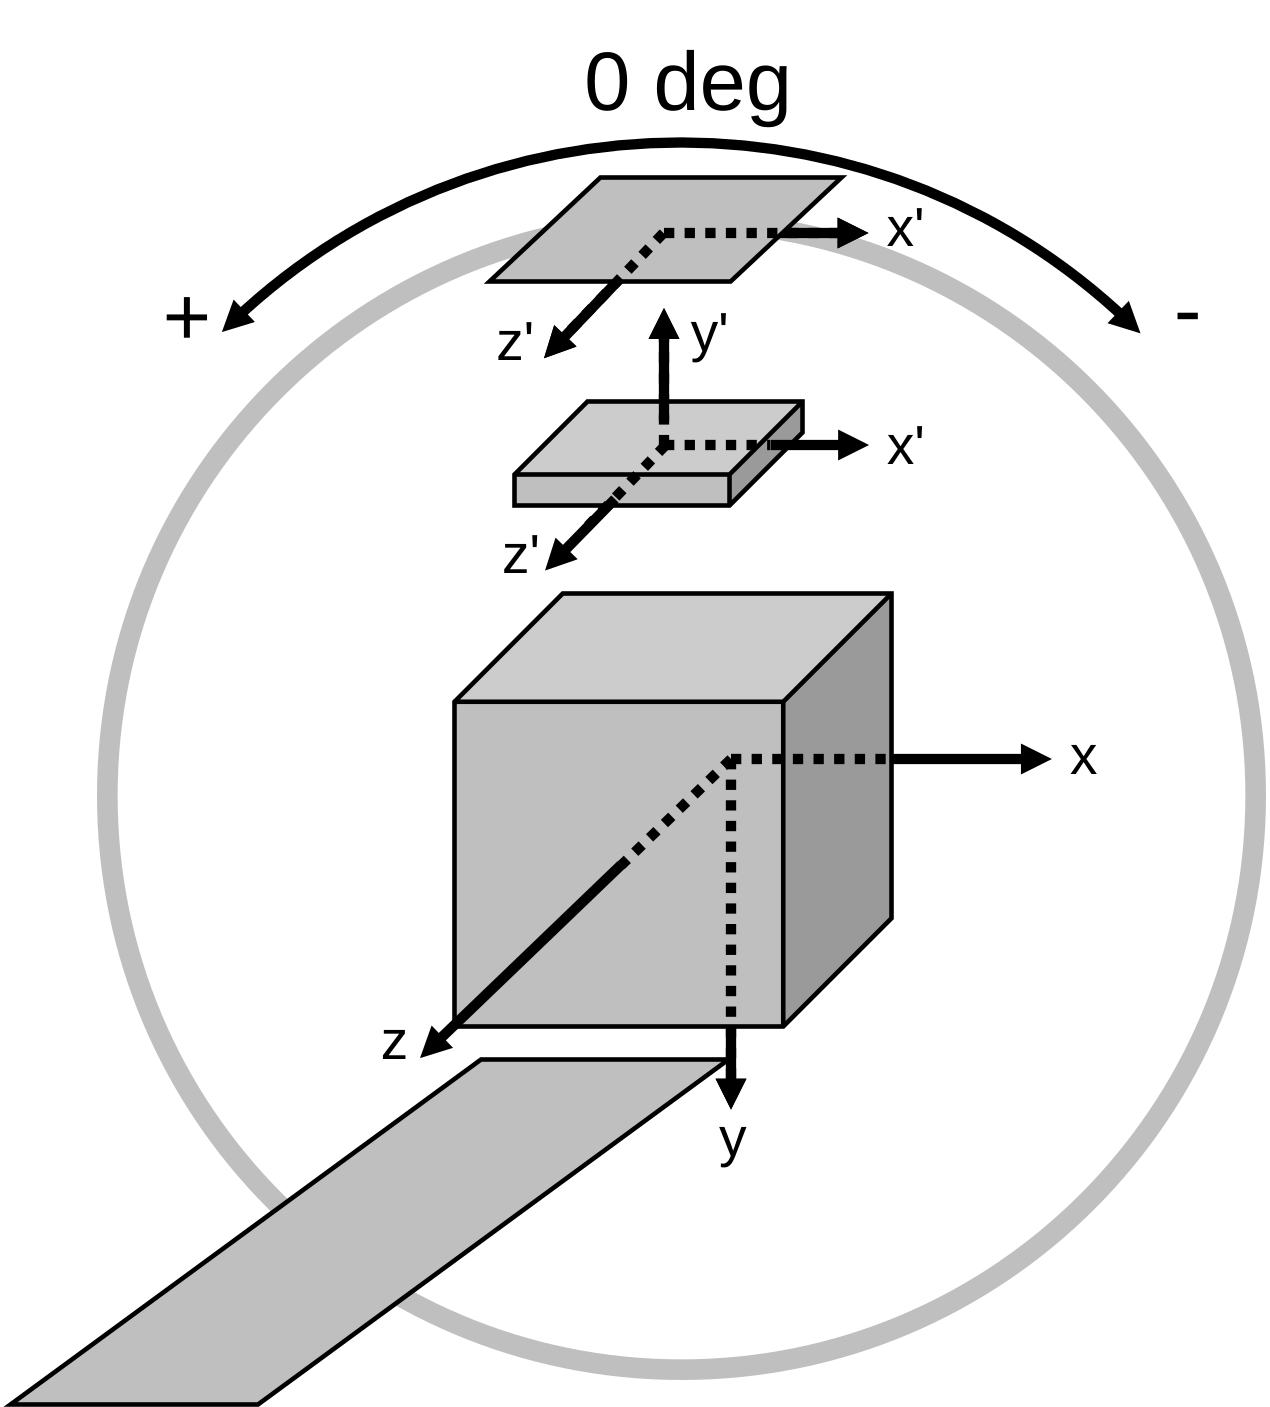
\includegraphics[height=5cm]{graphics/STIR-UsersGuide_PinholeSPECTUB}
\caption{PinholeSPECTUB system of reference and sign criteria illustrated for a polygonal collimator setup. Note that the projection matrix adheres to STIR's coordinate system as indicated by the x, y, and z axes. The detector and collimator use a rotating frame of reference where the transaxial x' and axial z' axes coincide with STIR's axes when the detector is at 0 $\mathrm{\deg}$. The collimator uses a right-handed coordinate system as indicated by the y' axis which points toward the detector. Further information is given in the parameter descriptions.}
\label{PinholeSPECTUB_coords}
\end{center}
\end{figure}

\begin{verbatim}
Projection Matrix By Bin Pinhole SPECT UB Parameters:=

   maximum number of sigmas := 2.0
   spatial resolution PSF := 0.001
   subsampling factor PSF := 1
   
   detector file := detector.txt
   collimator file := collimator.txt

   ; PSF and DOI correction { Yes // No }
   psf correction := no
   doi correction := no
   
   ; Attenuation correction { Simple // Full // No }
   attenuation type := no
   attenuation map :=
   
   object radius (cm) := 2.3
   mask file := 
   ; If no mask file is set, we can either compute it from attenuation map or object radius
   mask from attenuation map := 0
   
   keep all views in cache := 0

End Projection Matrix By Bin Pinhole SPECT UB Parameters:=
\end{verbatim}

{ \subsubsubsubsection{Parameters} }
\begin{description}

%\item[minimum weight:] Minimum weight to take into account (float, typically 0.0-0.02, default 0.0). It makes reference just to the geometric (PSF) part of the weight. The weight could be lower than this value after applying the attenuation factor.

\item[maximum number of sigmas:] Number of sigmas to consider when correcting for intrinsic PSF (float, typically 1.5–2.5, default 2.0). To increase unnecessarily the number of sigma would produce an increase of the weight matrix size that would not result in a better PSF correction. PSFs are modelled by Gaussian functions whose extension is infinite. It does not make sense to take into account very small contribution. A balance between the precision of the correction for PSF and the size of the matrix and the time of the reconstruction process should be done.

\item[spatial resolution PSF:] This is the spatial high resolution in which to sample distributions (float, cm, typically 0.001-0.0001, default 0.001, depends on the voxel size). It applies to geometric, PSF, and DOI calculations. The geometric contribution to one bin is the plane integral of the shadow of the hole within the bin. To easily compute thousands of integrals, the code pre-calculates the cumulative sum of the shadow of the hole at high resolution. This parameter indicates the discretization interval for such functions. The smaller this parameter the longer it takes to calculate the DOI correction (linear proportion).

\item[subsampling factor PSF:] This is the subsampling factor to compute convolutions when PSF or DOI corrections are enabled (integer, typically 1-8, default 1). In some cases, the Gaussian that describes the intrinsic PSF has just a few voxels. To convolve the shadow of the hole with a low resolution intrinsic PSF could have low accuracy. The subsampling factor reduces temporally the resolution of the PSF to perform more accurate calculus and then down sample the final PSF to the bin size. It has a great influence on the computation time.

\item[detector file:] Name of the file containing the detector information. See below for information on the structure of this file.

\item[collimator file:] Name of the file containing the collimator information. See below for information on the structure of this file.

\item[psf correction:] \{Yes, No (default)\} Enable or disable corrections for intrinsic PSF.

\item[doi correction:] \{Yes, No (default)\} Enable or disable corrections for DOI. \textbf{Note:} There is currently a bug associated with the DOI correction at small angles from the pinhole axis.

\item[attenuation type:] \{Simple, Full, No (default)\} Attenuation is calculated as the negative exponential of the sum of the length of the projection ray in each crossed voxel by its attenuation coefficient. It requires an attenuation map (see next parameter). The simple option for correction for attenuation is to consider that the whole PSF suffers the same attenuation (the attenuation of the central ray). One single factor is applied to weight the contribution from one voxel to all the bins in a detection plane. It is a very good approximation for uniform attenuation maps. The full option means that a different attenuation coefficient is calculated for each voxel-bin contribution (that is obtained along the voxel-bin pathway). It could be useful for very inhomogeneous attenuation maps.

See [Fus14] for an evaluation and more explanation.

\item[attenuation map:] A filename giving the attenuation map as the attenuation coefficient at each voxel (in $\mathrm{cm}^{-1}$). If the attenuation map is provided but the attenuation type is set to ``No'', then simple attenuation will be applied automatically. Currently, this file has the same geometric characteristics as the image to be reconstructed (number of columns, rows, slices, voxel dimensions, and orientation).

\item[object radius (cm):] The radius of the object in the xy plane of the image volume. All voxels belonging to this cylinder are weighted according to this radius whether or not a mask is used. If a mask is not used, all voxels outside of this cylinder are masked by default. If a mask is specified, this radius should be no smaller than the object in the mask volume to avoid errors in the geometric or convolution calculation of the PSF. See the following two parameters for more information.


%\item[mask type:] \{Attenuation Map, Explicit Mask, No (default)\} Applying a mask to the image volume reduces the matrix size by removing weights from voxels that do not contribute to the projections. The cylindrical mask is applied by default according to the object radius. This parameter applies additional masking. Possible values are:

%\begin{description}

%\item[Attenuation Map:] The attenuation map is used as a mask. No weight is calculated where the attenuation map is zero (no attenuation = no activity). If the attenuation map is obtained from a time-activity curve, very small values of attenuation could be set around the subject. Thresholding the attenuation map could be considered to adjust the mask to the subject. NaNs values are set to zero.
%\item[Explicit Mask:] The mask is defined in a file. The mask should have the same geometrical characteristics as the image. It could be useful, for instance, to remove the weight of voxels from the patient table (no activity but attenuation) or to reduce the matrix size when no attenuation for correction is considered. If not, attenuation map should suffice.

%\item[No:] No additional masking.

%\end{description}

\item[mask file:] Applying a mask to the image volume reduces the matrix size by removing weights from voxels that do not contribute to the projections. If a mask file is provided, any voxels which are (exactly) zero in the mask will be ignored during reconstruction. It could be useful, for instance, to remove the weight of voxels from the patient table (no activity but attenuation) or to reduce the matrix size when no attenuation correction is considered. If not, attenuation map should suffice. If no mask file is set, masking will be applied either either outside of the object radius, or with the attenuation map (see next parameter).  Currently, this file has the same geometric characteristics as the image to be reconstructed (number of columns, rows, slices, voxel dimensions, and orientation).

\item[mask from attenuation map:]  [0,1,0{]} If this variable is set to 0 (default), then masking will be applied either outside of the object radius, or with the mask file if it is set (see previous parameter). If this variable is set to 1 and no mask file is provided, then the attenuation map will be used to mask the image volume. No weight is calculated where the attenuation map is zero (no attenuation = no activity). If the attenuation map is obtained from a time-activity curve, very small values of attenuation could be set around the subject. Thresholding the attenuation map could be considered to adjust the mask to the subject. NaNs values are set to zero. \textbf{Note:} If this variable is set to 1 AND the mask file is specified, then this parameter will be automatically set to 0.

\item[keep all views in cache:] [0,1,0{]} If this variable is set to 0 (default), only a single view is kept in memory. This avoids running out-of-memory but means that the matrix has to be recomputed at every iteration.

\end{description}

{ {\subsection*{{Detector file} }
This file contains information about projections (see Fig.~\ref{PinholeSPECTUB_coords} for projection image orientation and angle criteria). Parameters are defined with a delimiting colon ``:". The labels before the colon are just information for users. The colon indicates the following value is a parameter to read, so it should be avoided in comments. The parameters should always keep the same order because they are read sequentially. The structure is demonstrated below with settings for the Cubresa Spark preclinical SPECT system in an aquisition with four projections over 360 degrees (see [Str22b]).

\begin{verbatim}
Information of detector
Comments are allowed here or anywhere in lines not containing parameters.
Parameters are defined with a delimiting colon. Avoid using a colon elsewehere.
# Sigma = FWHM/(2*sqrt(2*ln(2))) where FWHM = 0.85 mm
# CsI at 140.5 keV from NIST
Number of rings: 1
#intrinsic PSF#
Sigma (cm): 0.0361
Crystal thickness (cm): 0.3
Crystal attenuation coefficient (cm -1): 4.407   
\#……repeat for each ring …………\#
Nangles: 4
ang0 (deg): 180.
incr (deg): 90.0
z0 (cm): 0.
\#…………until here……………\#
\end{verbatim}

\noindent Note that detector radius (in mm), projection matrix size, and scaling factor (mm/pixel) are read directly from the Interfile header. The detector radius refers to the front of the crystal (external face). In case of no DOI correction, the program automatically adds half of the crystal thickness to the detector radius. The projection matrix size can be different in the axial and transaxial directions. The code works internally in radians although the angular parameters in input files are specified in degrees. This file should contain all the parameters although not used for that particular matrix. If not, indices will not match.

{ \subsubsubsubsection{Parameters} }
\begin{description}

\item[Number of rings:] There can be several rings of detectors. Each one can have a different configuration according to the parameters for Nangles, ang0($\mathrm{\deg}$), incr($\mathrm{\deg}$), and z0($\mathrm{cm}$).

\item[Sigma (cm):] Sigma $\sigma$ defines the standard deviation of the Gaussian that describes the intrinsic PSF. It can be calculated from the intrinsic resolution (FWHM) of the system as 
\begin{equation}
 \sigma = \frac{\mathrm{FWHM}}{2\sqrt{2\ln{2}}}.
\end{equation}

\item[Crystal thickness (cm):] Thickness of the scintillating crystal.

\item[Crystal attenuation coefficient (cm -1):] Attenuation coefficient of the crystal for the photon energy of interest.

\item[Nangles:] Number of angles for projection images stored in the current detector ring.

\item[ang0 (deg):] Starting angle of the detector in the current detector ring where the first projection was acquired. For example, 0 $\mathrm{\deg}$ refers to a detector above the patient table and 180 $\mathrm{\deg}$ refers to a detector below the patient table.

\item[incr (deg):] Angular increment of the detector between projections in the current detector ring. When looking from the patient table into the gantry, a positive angular increment refers to a CCW rotation.

\item[z0 (cm):] This refers to the axial position of the detector in the current ring relative to the center of the image volume.

\end{description}

{ {\subsection*{{Collimator file} }
This file contains information about projections (see Fig.~\ref{PinholeSPECTUB_coords} for collimator/pinhole orientation and angle criteria). Parameters are defined with a delimiting colon. The labels before the colon are just information for users. The colon indicates the following value is a parameter to read, so it should be avoided in comments. The parameters should always keep the same order because they are read sequentially. The structure is demonstrated below with settings for the Cubresa Spark preclinical SPECT system in an aquisition with four projections over 360 degrees and a single-pinhole collimator (see [Str22b]).

\begin{verbatim}
Information of collimator
Comments are allowed here or anywhere in lines not containing parameters.
Parameters are defined with a delimiting colon. Avoid using a colon elsewehere.
Model (cyl/pol): pol
Collimator radius (cm): 2.8
Wall thickness (cm): 1.
#holes#
Number of holes: 4
nh / ind / x(cm) / y(cm) / z(cm) / shape(rect-round) / sizex(cm) / sizez(cm)
/ angx(deg) / angz(deg) / accx(deg) / accz(deg)
h1:	1	0.	0.	0.	round	0.1	0.1	0.	0.	45.	45.
h2:	2	0.	0.	0.	round	0.1	0.1	0.	0.	45.	45.
h3:	3	0.	0.	0.	round	0.1	0.1	0.	0.	45.	45.
h4:	4	0.	0.	0.	round	0.1	0.1	0.	0.	45.	45.
\end{verbatim}

{ \subsubsubsubsection{Parameters} }
\begin{description}

\item[Model (cyl/pol):] The collimator could be either cylindrical or polygonal (flat faces). In both cases, the holes are supposed to be parallel to detector plane.

\item[Collimator radius (cm):] In case of polygonal collimator, the radius refers to the apothem, i.e., radius of rotation. This is the radial distance from the central axis to the center of the face of the collimator.

\item[Wall thickness (cm):] Thickness of the face of the collimator.

\item[Number of holes:] The number of holes is the total, considering all angular projections and rings. 

\item[nh:] For each hole, the following information should be introduced in rows (value previous to ``:" is a label and is not read).

\begin{description}

\item[ind:] Index from 1 to the number of detector elements defining which detection element the hole projects to. In case one hole projects to more than one detector element, it should be added twice, once for each detector element using the relative position to that detector element. Assign the same detector element index to different holes to indicate that they project to the same detector element.

\item[x, y, z coordinate (cm):] \textit{Polygonal collimator:} Center of the hole in the collimator plane. That is, 0. 0. 0. refers to the middle of the collimator face and in the middle of the collimator wall. Coordinates x, z refer to spatial position in the plane (transaxial and axial, respectively) and y is the radial position of the hole in the wall thickness, so it should be kept between $\pm$~wall\_thickness/2. \textbf{Note:} The collimator coordinate system is a right-handed coordinate system (see Fig.~\ref{PinholeSPECTUB_coords}). When the detector and collimator are at 0 $\mathrm{\deg}$, the axial and transaxial axes coincide with STIR's coordinate system whereas the collimator y-axis points radially outward toward the detector. \\ \textit{Cylindrical collimator:} Replace x(cm) y(cm) z(cm) with ang(deg) y(cm) z(cm) for cylindrical coordinates. 

\item[shape (rect-round):] rect or round depending on if the hole has rectangular or round shape, respectively.

\item[x, z hole size (cm):] Hole dimensions in the x (transaxial) and z (axial) directions.

\item[x, z angle (deg):] Angle by which to tilt the central axis of the hole in the x and z directions. \textbf{Note:} The normal of a pinhole with a 0 $\mathrm{\deg}$ tilt lies along the y-axis (i.e., pointing toward the detector). A positive tilt angle will rotate the normal toward the indicated axis by the defined amount.

\item[x, z acceptance angles (deg):] Aperture with respect to the hole axis given by half of the total acceptance angle.

\end{description}
\end{description}


{ \subsubsubsection{From File} }
\label{sec:projmatrixfromfile}
You can use \texttt{write\_proj\_matrix\_by\_bin} to write a projection matrix to file. You can
then read the matrix back into memory. This
could be useful if it takes a long time to generate the matrix, or if you have an external program
to write the matrix (see below for more information on what you will need to do).


{ \subsubsubsubsection{Parameters}
}
The necessary parameters to include in the par file are:
\begin{verbatim}
ProjMatrixByBinFromFile Parameters:=
  Version := 1.0
  symmetries type := PET_CartesianGrid
    PET_CartesianGrid symmetries parameters:=
      do_symmetry_90degrees_min_phi:= <bool>
      do_symmetry_180degrees_min_phi:=<bool>
      do_symmetry_swap_segment:= <bool>
      do_symmetry_swap_s:= <bool>
      do_symmetry_shift_z:= <bool>
    End PET_CartesianGrid symmetries parameters:=
  ; example projection data of the same dimensions as used 
  ; when constructing the matrix
  template proj data filename:= <filename>
  ; example image of the same dimensions as used 
  ; when constructing the matrix
  template density filename:= <filename>
  ; binary data with projection matrix elements
  data_filename:=<filename> 
End ProjMatrixByBinFromFile Parameters:=
\end{verbatim}
The symmetries all default to true, but it is best to include the values in the file in all cases. 

You need to be careful that these parameters match the matrix written to file. To make this easier,
\texttt{write\_proj\_matrix\_by\_bin} will write these to file for you. In the current version
of STIR, you will need to copy these into the .par file (this will change in a future version of STIR).

Note that image and projection data characteristics are read from the \texttt{template} files. Their geometric
characteristics have to match those of the data that you want to process with the stored matrix
(the stored matrix could have more segments or tangential positions than the data). This will be
checked at run-time.

{ \subsubsubsubsection{Information on how to write your own projection matrix to file}
}
The projection matrix is stored as a sparse matrix (in the file dennoted by the \texttt{data\_filename}
parameter). The format is reasonably simple. For each element (``bin'') in the projection data, the 
Line of Response (LOR) is encoded as follows:
\begin{verbatim}
  segment_num (int32_t)
  view_num (int32_t)
  axial_pos_num (int32_t)
  tangential_pos_num (int32_t)
  num_voxels_in_LOR (uint32_t)
  for_each voxel
     z (int16_t)
     y (int16_t)
     x (int16_t)
     matrix_value (float)
  end
\end{verbatim}
The order of bins is not important, neither is the order of the voxels (although you will get better
performance if these are stored such that voxels are listed consecutively).

To reduce data size, symmetries can be used to store only ``basic'' Lines Of Responses (LORs). 
The exact definition of the symmetries is unfortunately
not easy and not documented fully here. If you want to use your own code to write the matrix and want to use
symmetries you will need to check the \texttt{DataSymmetriesForBins} class or a derived class. In case all
symmetries are enabled, the following should hold:
\begin{verbatim}
0<=segment_num
0<=view_num<=num_views/4
axial_pos_num==0
0<=tangential_pos_num
\end{verbatim}
Check the STIR developer's guide and the Wiki for information on coordinate systems used by STIR. In particular,
note the STIR convention about index numbering in section 2.2 of the developer's guide.

A final note: currently the sparse matrix is read completely into memory before it is used (but of course
keeping only the ``basic'' part of the matrix taking the symmetries into account). This restricts the size
of the matrix according to how much memory your system has available.

\subsubsection{
Selecting a bin normalisation procedure}
\label{sec:binnormalisation}
In PET, a procedure called 'normalisation' is used which is essentially 
a calibration procedure for every detector pair. It provides 
a multiplicative factor for every bin, or element of the projection 
data.\\
The library can provide different types of normalisation procedures. 
It is possible to select these independently at run-time, and 
extend the available ones at compile time. The mechanism is exactly 
the same as for the ForwardProjector hierarchy.


In addition to the types listed below, you can also enter 'None', 
which means that the data won't be normalised at all.

{ \subsubsubsection{From Projdata}
}\label{sec:binnormalisationFromProjData}
This can be used when the normalisation factors are stored simply 
as projection data. Currently, these data have to have exactly 
the same characteristics (size etc.) as the projection data which 
are going to be normalised. Note that the stored factors have 
to be the ones you'd apply to normalise the data (and not their 
reciprocal).

{ \subsubsubsubsection{Parameters}
}
\begin{verbatim}
Bin Normalisation From ProjData :=
normalisation projdata filename:= norm.hs
End Bin Normalisation From ProjData:=
\end{verbatim}

See also online documentation for class BinNormalisationFromProjData.

{ \subsubsubsection{From ECAT7}
}
This can be used when normalising ECAT7 data. CTI/Siemens stores
the normalisation data in a files normally ending on
\texttt{.n} or \texttt{.N}. Dead-time correction is also
supported, although awkwardly. To get dead-time correction
to work, you need to specify the singles rates for the 
scan\footnote{In future, hopefully this will not be necessary.
This work-around is needed because \textit{STIR} currently does not
directly read any of the meta-data in the headers of sinograms etc.}
{ \subsubsubsubsection{Parameters}
}
\begin{verbatim}
Bin Normalisation From ECAT7:=
  normalisation filename:= STUDY.n
  singles rates := Singles From ECAT7 File
  Singles Rates From ECAT7 File:=
      ECAT7_filename := ecat7_sinogram.S
  End Singles Rates From ECAT7:=
End Bin Normalisation From ECAT7:=
\end{verbatim}

In addition, you currently have to set the time frame information in the .par file.

See also online documentation for class BinNormalisationFromECAT7.

{ \subsubsubsection{From Attenuation Image}
}
\label{sec:binnormalisationfromattenuationimage}
This can be used for attenuation correction factors (ACFs) if 
you do not have the ACFs but an attenuation image (or mu-map). 
The ACFs are found by forward projecting the attenuation image, 
multiplying the result with -1, and exponentiating, i.e. using 
Beer's law.



\textbf{Warning} Attenuation image data are supposed to be in units \textit{cm}$^{-1}$. 
(Reference: water has $\mu=.096 \mathit{cm}^{-1}$.)

{ \subsubsubsubsection{Parameters}
}
\begin{verbatim}
Bin Normalisation From Attenuation Image:=
attenuation_image_filename := <string>
forward projector type := <string>
End Bin Normalisation From Attenuation Image :=
\end{verbatim}


Default forward projector is ForwardProjectorByBinUsingRayTracing 
(see section \ref{sec:forwardprojectors}).


See also online documentation for class BinNormalisationFromAttenuationImage.

{ \subsubsubsection{Chained }
}
\label{sec:chainedbinnormalisation}
This can be used to apply two normalisation one after the other. 
For example, a first one could be the 'usual' normalisation factor, 
while a second one could be the attenuation factors.

{ \subsubsubsubsection{Parameters}
}
\begin{verbatim}
Chained Bin Normalisation Parameters:=
Bin Normalisation to apply first:= some_bin_normalisation_type
; parameters for this type

Bin Normalisation to apply second:= some_bin_normalisation_type
; parameters for this type

END Chained Bin Normalisation Parameters:=
\end{verbatim}

See also online documentation for class \texttt{ChainedBinNormalisation}.

{ \subsubsubsection{SPECT }
}
\label{sec:SPECTbinnormalisation}
This can be used to apply decay correction and uniformity for SPECT. You need to specify the folder where the data and uniformity table are. In addition, for the decay correction it is necessary to specify how many detector heads the scanner has, the acquisition time per angular position, and  the half life of the radioisotope.

{ \subsubsubsubsection{Parameters}
}
\begin{verbatim}
Bin Normalisation type := SPECT
   Bin Normalisation SPECT:=
      folder_prefix:=folder_prefix
      projdata filename:=input_sino
      use_uniformity_factors :=0
      uniformity_filename:=uniformity_table.dat
      use_decay_correction:=1
     
      half_life:=21600 ;seconds
      num detector heads:=3
      rel_angle:=120
      
      ;the following is the time of a head position
      view_time_interval:=15 ;seconds

   End Bin Normalisation SPECT:=
\end{verbatim}


\subsubsection{
Available shapes}
\label{sec:shapes}
\textbf{STIR} can use shapes, \textit{e.g.} in the \texttt{generate\_image}
utility (see section \ref{sec:generate_image}), or for specifying ROIs, see \ref{sec:list_ROI_values}.
The distribution contains sample parameter files in the
\texttt{samples} directory. In the following sub-sections the available shapes are listed.

Most shapes have a centre and orientation. This is specified in the parameter files
by giving the ``origin'' and a $3x3$ matrix specifying $3$ direction vectors.
Note that these vectors do not necessarily have to be orthogonal nor have unit-norm.
To decide if a point with coordinates \texttt{coords} is inside the shape, the
coordinates are first translated to ``shape-specific'' coordinates using:
\[
\mathtt{shape\_coords} = \mathtt{direction\_vectors}. (\mathtt{coord}-\mathtt{origin})
\]

When parsing, the relevant variables are specified as follows:
\begin{verbatim}
    origin (in mm):= <float> ;defaults to {0,0,0}
     ; values below are give a rotation around y for 90 degrees (swapping x and z)
     ; Warning: this uses the STIR convention {z,y,x}
     direction vectors (in mm) := { {0,0,1}, {0,1,0}, {-1,0,0}}
\end{verbatim}

See also the online documentation for the class \textbf{Shape3D} and
\textbf{Shape3DWithOrientation}.

{ \subsubsubsection{Box3D}
}
Three-dimensional cuboid box.
{ \subsubsubsubsection{Parameters}
}
\begin{verbatim}
  Box3D Parameters:=
     length-x (in mm):= <float>
     length-y (in mm):= <float>
     length-z (in mm):= <float>
     ; any parameters of Shape3DWithOrientation
  End:=
\end{verbatim}

{ \subsubsubsection{Ellipsoid}
}
Three-dimensional ellipsoid.
A point with coordinates ``shape-coordinates'' $x,y,z$ is inside the shape if
\[
  {x^2 \over R_x^2} + {y^2 \over R_y^2} + {z^2 \over R_z^2} \le 1
\]
{ \subsubsubsubsection{Parameters}
}
\begin{verbatim}
   Ellipsoid Parameters:=
     radius-x (in mm):= <float>
     radius-y (in mm):= <float>
     radius-z (in mm):= <float>
     ; any parameters of Shape3DWithOrientation
   End:=
\end{verbatim}

{ \subsubsubsection{Ellipsoidal Cylinder}
}
Three-dimensional ellipsoidal cylinder (oriented along the z-axis).
A point with coordinates ``shape-coordinates'' $x,y,z$ is inside the shape if
\[
  {x^2 \over R_x^2} + {y^2 \over R_y^2}  \le 1 \,\,\,\, \mathrm{and}  \,\,\,\,\mathrm{abs}(z) \le L_z/2
\]
In addition, this shape can be restricted to a wedge by specifying initial and final angles (w.r.t. the $x$ axis).
\subsubsubsubsection{Parameters}
\begin{verbatim}
   Ellipsoidal Cylinder Parameters:=
     radius-x (in mm):= <float>
     radius-y (in mm):= <float>
     length-z (in mm):= <float>
     initial angle (in deg):= <float> ; (defaults to 0)
     final angle (in deg):= <float>   ; (defaults to 360)
     ; any parameters of Shape3DWithOrientation
   End:=
\end{verbatim}

{ \subsubsubsection{Discretised Shape3D}
}
This shape can be used to read for instance saved ROIs. This class supports 2 options:
\begin{itemize}
  \item a label-image with associated label index (an integer), suitable for multiple ROIs in a single file.
  \item a ``weight" image, with (potentially) smooth edges, where voxel values
    are supposed to be between $0$ and $1$.
\end{itemize}
Note that centre and orientation are taken from the image data, not from the parameter file.
{ \subsubsubsubsection{Parameters}
}
\begin{verbatim}
  Discretised Shape3D Parameters:=
    input filename := <filename>
    ; optional member (if not set, or negative, STIR will use the image as weights
    label index := <int>
  END:=
\end{verbatim}
where \texttt{filename} needs to specify a volume that can be read by STIR.


\subsection{
Display}\label{sec:display}
Some of the programs (e.g. in utilities/, recon\_tests/) use 
the display routines. Which version is actually used depends 
on the compilation settings (in particular the \textit{GRAPHICS} cmake 
variable), see section \ref{sec:UsingCMake}. 


\subsubsection{
X Windows display}
\label{sec:displayX}
\textbf{Warning} This functionality is deprecated and will be removed in STIR v7.0.

This provides a (very basic) way of displaying bitmaps when using 
X windows. This works by creating a new window where some of 
the bitmaps are displayed. To proceed, you have to make this 
window the 'focus' (how to do this depends on your window manager 
but usually you have to move the cursor over it, or click the 
title bar) and then press any key. In your original terminal 
window you will then be asked if you want to continue with the 
next set of bitmaps until no more are left.


In addition, when your X server supports the Pseudocolor visual, 
you can cycle between 4 different colour scales by pressing Mouse 
button 2 while the 'bitmap' window is selected.


\textbf{Warning} In the current implementation, it seems to happen 
occasionally that not all colours in the colour scale have been 
allocated properly. This can be seen by looking at the side bar 
displaying the colour scale. Unfortunately, this effect might 
give you wrongly coloured regions (usually spots) in the image.


\subsubsection{
PGM display}

This 'display' mode actually writes out a file in the Portable 
Greyscale Map format, which can be read by various graphics programs 
(like Paint Shop Pro or xv).


\subsubsection{
MathLink display}

This mode is (somewhat) useful if you have \textit{Mathematica\texttrademark}, 
and want to pipe the data into \textit{Mathematica}. (It is probably 
easier to read the binary data from file though using the \textit{Mathematica} command \texttt{BinaryRead}). 
Sample \textit{Mathematica} statements:

\begin{verbatim}
(* create link before starting the (first) display in your STIR 
program*)

link=LinkCreate[``STIR''];

(* read data from link *)
data3d=LinkRead[link];


(* display the 3rd image *)
ListPlot3D[data3d[[3]], Mesh->False];
(* read data from link from next display *)
nextdata3d=LinkRead[link];
(* and so on *)

(* close link at end of STIR program *)
LinkClose[link];
\end{verbatim}


\section{B-spline interpolation in STIR}

\label{sec:BSplines}
Special classes to interpolate data using B-Splines [Uns99] have been implemented in STIR. 
The B-Splines coefficients are estimated with a fast method that incorporates FIR and IIR 
filters [Uns93]. The level of B-splines that are currently available are 0, 1 (linear), 
2 (quadratic), 3 (cubic), 4 (quartic) and 5 (quintic). Moreover, a synthetic spline has also been 
implemented based on B-splines for maximum order interpolation but minimal support, i.e. MOMS 
splines [Blu01]. In all cases no regularization has been incorporated during the interpolation 
procedures, therefore special care should be taken when higher than the first order B-splines 
are used, as noise may be enhanced at the interpolated data. Interpolation can be also performed 
in sinogram space. However this space is regular only in axial, and not in radial, angular and 
azimuthal directions. Therefore, the current interpolation can be cubic only in axial direction 
while for the rest directions a choice of linear interpolator is safer. In future with some 
additional classes, reconstruction could be performed to obtain B-spline coefficients directly 
from the projection sinograms, which can be useful for better noise properties [Nic02].

\section{
Directories in the STIR tree}
\textit{STIR} can roughly be split into a library applications and applications.
\footnote{The distinction is not complete as some applications are implemented
in terms of classes that actually end up in the library.}

See the doxygen documentation for an overview of the directory tree with brief descriptions.

\section{Using STIR in an external C++ project
\label{sec:ExternalProjectC++}}
STIR exports its CMake settings. Therefore, an external project can do
\begin{verbatim}
find_package(STIR 6.0 REQUIRED CONFIG)
add_library(my_lib file1.cxx file2.cxx)
# my_lib uses STIR functionality
target_link_libraries(my_lib PUBLIC ${STIR_LIBRARIES})
add_executable(my_exe my_exe.cxx ${STIR_REGISTRIES})
target_link_libraries(my_exe PUBLIC my_lib))
\end{verbatim}
In addition, if your CMake is older than 3.12, you need to add
\begin{verbatim}
include_directories("${STIR_INCLUDE_DIRS}")
\end{verbatim}
to your CMakeLists.txt file to get the source code files listed in \texttt{STIR\_REGISTRIES} to compile.
(For more recent CMake, this should not be necessary (as \texttt{STIR\_REGISTRIES} is set to
a list of compiled files).

A fully working example is provided in the \texttt{examples/C++} folder, see also the
\url{https://github.com/UCL/STIR/tree/master/examples/C\%2B\%2B/using_installed_STIR}{using\_installed\_STIR folder on GitHub}.

Note that if CMake did not find the STIR files, you can point it to where they are installed.
For example, if you installed STIR with
\texttt{CMAKE\_INSTALL\_PREFIX=\$HOME/install}, set
\texttt{CMAKE\_PREFIX\_PATH=\$HOME/install} or \texttt{STIR\_DIR=\$HOME/install/lib/cmake/STIR-6.0}.
\footnote{This uses CMake Config mode for \texttt{find\_package}. There is no need for a \texttt{FindSTIR.cmake}}

\section{
Future developments and Support}

The \textit{STIR} library, in its current state, possesses many capabilities. 
The developers, however, look forward to still further increases 
in the flexibility and power of the software.
Please check the \url{https://github.com/UCL/STIR/milestones}{GitHub milestones}
for some information.


While support for the library is on a voluntary basis, users 
of the library are encouraged to subscribe to relevant \textit{STIR} 
mailing lists (see the `Mailing Lists' section of the \textit{STIR} website 
\url{http://stir.sourceforge.net/ }{http://stir.sourceforge.net}) 
where they can follow developments of the software and obtain 
helpful information from other users. Questions will ONLY be 
answered (if at all) when creating a \url{https://github.com/UCL/STIR/issues}{GitHub issue} (preferred) or
when directed to the mailing list.

Commercial support is available from \url{http://asc.uk.com}{Algorithms and
Software Consulting Ltd}.




\section{
References}

\tab {[}Ahn2003] S. Ahn and J. A. Fessler, \textit{Globally convergent image reconstruction for
emission tomography using relaxed ordered subsets algorithms,} IEEE
Trans. Med. Imag., vol. 22, no. 3, pp. 613-626, May 2003.

{[}Ale97] Alenius S and Ruotsalainen U \textbf{(1997)} Bayesian image 
reconstruction for emission tomography based on median root prior. \textit{European 
Journal of Nuclear Medicine} , Vol. 24 No. 3: 258-265.

{[}Ang11] Angelis G I, Thielemans K, Tziortzi A C, Turkheimer F E and Tsoumpas C  
\textbf{(2011)}. Convergence Optimization of Parametric MLEM Reconstruction for Estimation of Patlak Plot Parameters.  
\textit{Computerized Medical Imaging and Graphics}, 35:407-416,  
\textit{doi:10.1016/j.compmedimag.2011.01.002}

{[}Ben99] Ben-Tal A, Margalit T and Nemirovski A \textbf{(1999)} The 
ordered subsets mirror descent optimization method with application 
to tomography. \textit{Research report \#2/99, March 1999, MINERVA 
Optimization Center, Faculty of Industrial Engineering and Management, 
Technion -- Israel Institute of Technology}.

{[}Ben99b] Ben-Tal A and Nemirovski A \textbf{(1999)} The conjugate 
barrier method for non-smooth, convex optimization. \textit{Research 
report \#5/99, October 1999, MINERVA Optimization Center, Faculty 
of Industrial Engineering and Management, Technion -- Israel Institute 
of Technology.}

[Bei08] Beisel T, Lietsch S, and Thielemans K \textbf{(2008)}
A Method for OSEM PET Reconstruction on Parallel Architectures Using STIR.
\textit{Proc. of the IEEE Medical Imaging Conference, Dresden, Germany, 2008}.

{[}Blu01] Blu T, Thcvenaz P, Unser M \textbf{(2001)}. MOMS: maximal-order interpolation of minimal support.  \textit{IEEE Trans Image Processing} 10(7): 1069-1080.

[Bue12] Buerger, C., T. Schaeffter, and A. P. King \textbf{(2011)}, Hierarchical adaptive
local affine registration for fast and robust respiratory motion estimation.
Medical Image Analysis, vol. 15, pp. 551-564, 
\url{http://dx.doi.org/10.1016/j.media.2011.02.009}{doi 10.1016/j.media.2011.02.009} 

{[}Bou97] Boudraa \textsc{A E O} \textbf{(1997)} Automated detection of the 
left ventricular region in magnetic resonance images by Fuzzy 
C-Means model. \textit{Int J of Cardiac Imag} ; 13: 347-355.

{[}Dau86] Daube-Witherspoon M E and Muehllener G \textbf{(1986)} An 
iterative space reconstruction algorithm suitable for volume 
ECT. \textit{IEEE Trans. Med. Imaging}, vol. MI-5: 61-66.

{[}Dau97] Daube-Witherspoon M E and Muehllehner G \textbf{(1987)} 
Treatment of axial data in three-dimensional PET, 
J. Nucl. Med. 28, 171-1724.

{[}Def95] Defrise M. \textbf{(1995)} ``A factorization method for the 
3D X-ray transform'' \textit{Inverse Problems,} \textbf{11} pp. 983-994.


{[}Def97] Defrise M, Kinahan P E, Townsend D W, Michel C, Sibomana 
M and Newport D F \textbf{(1997)} Exact and approximate rebinning 
algorithms for 3-D PET data. \textit{IEEE Trans. Med. Imaging}, MI-16: 
145-158.

{[}Egg98] Egger M L, Joseph C and Morel C \textbf{(1998)} Incremental 
beamwise backprojection using geometrical symmetries for 3D PET 
reconstruction in a cylindrical scanner geometry. \textit{Phys Med. 
Biol.}, 43: 3009-3024.

{[}Ehr16{]} Ehrhardt M J, Markiewicz P, Liljeroth M, Barnes A, Kolehmainen V, Duncan J, Pizarro L, Atkinson D, Hutton B F, Ourselin S, and others \textbf{(2016)}, 
PET reconstruction with an anatomical MRI prior using parallel level sets. \textit { IEEE Trans Med Imaging } 35(9): 2189-2195.

{[}Gem84] Geman S and Geman D \textbf{(1984)} Stochastic relaxation, 
Gibbs distributions, and the Bayesian restoration of images. \textit{IEEE 
Trans PAMI}, 6: 721-741.

{[}Gem85] Geman S and McClure D \textbf{(1985)} Bayesian image analysis: 
an application to single photon emission tomography. \textit{in Proc. 
American Statistical Society, Statistical Computing Section (Washington, 
DC)} 12-18.


 {[}Gre90] Green P J \textbf{(1990)} Bayesian reconstruction from emission 
tomography data using a modified EM algorithm. \textit{IEEE Trans. 
Med. Imaging}, MI-9: 84-93.


{[}Heb89] Hebert T J and Leahy R M \textbf{(1989)} A generalized EM 
algorithm for 3-D Bayesian reconstruction from Poisson data using 
Gibbs priors. \textit{IEEE Trans. Med. Imaging}, MI-8: 194-202.


{[}Her80] Herman G T \textbf{(1980)} Image Reconstruction from Projections: 
The fundamentals of Computational Tomography. \textit{Academic Press, 
New York}.

{[}Hud94] Hudson H M and Larkin R S \textbf{(1994)} Accelerated image 
reconstruction using ordered subsets of projection data. \textit{IEEE 
Trans. Med. Imaging}, MI-13: 601-609.

{[}Fok2006] Fokas, A. S., A. Iserles, and V. Marinakis. "Reconstruction algorithm for
single photon emission computed tomography and its numerical implementation." \textit{Journal of the Royal Society Interface} 3.6 (2006).

{[}Fus13]  Berta Marti Fuster, Carles Falcon, Charalampos Tsoumpas, Lefteris Livieratos, Pablo Aguiar, Albert Cot, Domenec Ros and Kris Thielemans, \textbf{ (2013)} Integration of advanced 3D SPECT modeling into the open-source STIR framework, \textit{Med. Phys. 40}, 092502; http://dx.doi.org/10.1118/1.4816676.

{[}Fus14] Berta Marti Fuster, Kjell Erlandsson, Carles Falcon, Charalampos Tsoumpas, Lefteris Livieratos, Domenec Ros, Kris Thielemans, \textbf{(2014)}  Evaluation of the novel 3D SPECT Modelling Algorithm in the STIR Reconstruction Framework: Simple vs. full attenuation correction, \textit{proc. IEEE MIC 2013}, Seoul, Korea.

{[}Jac00] Jacobson M, Levkovitz R, Ben-Tal A, Thielemans K, Spinks 
T, Belluzzo D, Pagani E, Bettinardi V, Gilardi M C, Zverovich 
A and Mitra G \textbf{(2000)} Enhanced 3D PET OSEM Reconstruction 
using inter-update Metz filters. \textit{Phys. Med. Biol}. \textbf{45} No.8 
(2000) 2417-2439\textit{l.}


{[}Kin89] Kinahan P E and Rogers J G \textbf{(1989)} Analytic 3D image 
reconstruction using all detected events. \textit{IEEE Trans. Nucl. 
Sci.}, 36: 964-968.


[Kle96]
Klein, G. J., B. W. Reutter, and R. H. Huesman \textbf{(1996)}, Non-rigid summing of gated PET via optical flow, \textit{1996 IEEE Nuclear
Science Symposium Conference Record},
vol. 2, pp. 1339-1342, 
\url{http://dx.doi.org/10.1109/NSSMIC.1996.591692}{doi 10.1109/NSSMIC.1996.591692}

[Kyr2025]
Kyriakopoulou, D., A. Fokas, K. Thielemans \textbf{2025}, submitted to \textt{Inverse Problems}.

{[}Lab97] Labbe C, Ashburner J, Koepp M, Spinks T, Richardson M 
and Cunningham V \textbf{(1997)} Accurate PET quantification using 
correction for partial volume effects within cerebral structures. \textit{Neuroimage}, 
5: B12.


{[}Lab99a] Labb\'{e} C, Thielemans K, Belluzzo D, Bettinardi V, Gilardi 
MC, Hague DS, Jacobson MW, Kaiser S, Levkovitz R, Margalit T, 
Mitra G, Morel C, Spinks T, Valente P, Zaidi H and Zverovich A\textit{: 
An object-Oriented Library for 3D PET Reconstruction using Parallel 
Computing}, Proceedings of Bildverarbeitung fuer die Medizin 
1999, Algorithmen-Systeme-Anwendungen, \textit{Informatik} 
\textit{aktuell, Springer}, Eds. H. Evers, G. Glombitza, T. Lehmann, 
H.-P. Meinzer, pp 268-272. 

{[}Lab99b] Labb\'{e} C, Thielemans K, Zaidi H and Morel C: An object-oriented 
library incorporating efficient projection/backprojection operators 
for volume reconstruction in 3D PET\textit{. Proc. of 3D99 Conference}, 
June 1999, Egmond aan Zee, The Netherlands 


{[}Lal93] Lalush D S and Tsui M W \textbf{(1993)} A general Gibbs prior 
for Maximum a posteriori reconstruction in SPET. \textit{Phys. Med. 
Biol.}, 38: 729-741.

{[}Lan90] Lang K \textbf{(1990)} Convergence of EM Image reconstruction 
algorithms with Gibbs smoothing. \textit{IEEE Trans. Med. Imaging}, 
MI-9: 4.

{[}Lew98] Lewellen T K, Harrison R L and Vannoy S \textbf{(1998)} 
The SimSET program,
\textit{ Monte Carlo Calculations in Nuclear Medicine:
Applications in Diagnostic Imaging ed M Ljungberg, S-E Strand and M A King (Bristol: Institute of Physics
Publishing)} pp 77-92.

[Li06] Li, T., B. Thorndyke, E.
Schreibmann, \textit{et al} \textbf{(2006)}, Model-based image reconstruction for
four-dimensional PET. \textit{Med Phys} vol. 2, pp. 1288-1298
\url{http://link.aip.org/link/doi/10.1118/1.2192581}{doi 10.1118/1.2192581}

{[}Man97] Manders Jones H \textbf{(1997)} A Computational Investigation 
of the solution of large scale Optimization problems. \textit{Ph.D 
Thesis, Department of Mathematics and Statistics. Brunel, The 
University of West London. Oct 1997}.


{[}Mar99] Margalit T, Gordon E, Jacobson M, Ben-Tal A, Nemirovski 
A and Levkovitz R \textbf{(1999)} The ordered sets mirror descent and 
conjugate barrier optimization algorithms adapted to the 3D PET 
reconstruction problem. Technion internal report and PhD thesis of T. Margalit

[Mar18] Markiewicz P J, Ehrhardt M J, Erlandsson K, Noonan P J, Barnes A, Schott J M, 
Atkinson D, Arridge S R, Hutton B F, Ourselin S \textbf{(2018)}, 
NiftyPET: a High-throughput Software Platform for High 
Quantitative Accuracy and Precision PET Imaging and Analysis.
\textit { Neuroinformatics }, 16(1): 95-115.

{[}Mus01] Mustafovic S and Thielemans K, \textbf{(2001)} Additive and Multiplicative 
versions of the Maximum A Posteriori Algorithm with the Median 
Root Prior. poster at \textit{IEEE Med. Img. Conf. 2001.}

{[}Mus04] Mustafovic S and Thielemans K, \textbf{(200}\textbf{4}\textbf{)} \textit{Object 
Dependency of Resolution in Reconstruction Algorithms with Inter-Iteration 
Filtering Applied to PET} , IEEE Trans. Med. Im. 23 (4): (2004) 
433-446.

{[}Mus02] Mustafovic S and Thielemans K, \textit{,} \textbf{(2002)}  Comparison 
of Unconventional Inter-Filtering Methods to Penalised-likelihood 
for Space-invariant Tomographs, poster at \textit{IEEE Medical Imaging 
Conf. 2002}.

{[}Nem78] Nemirovski A and Yudin D \textbf{(1978)} Problem complexity 
and method efficiency in optimization. \textit{Nauka Publishers, 
Moscow, 1978 (in Russian); English translation: John Wiley \& 
Sons, 1983}.

{[}Nic02] Nichols, T. E., J. Qi, E. Asma and R. M. Leahy \textbf{(2002)}. Spatiotemporal reconstruction of list-mode PET data.  \textit{IEEE Trans Med Imaging} 21(4): 396-404.

{[}Pat83] Patlak C S, Blasberg R G, Fenstermacher J D \textbf{(1985)}  Graphical evaluation of blood-to-brain 
transfer constants from multiple-time uptake data. \textit{J Cereb Blood Flow Metab} 3(1): p. 1-7.

{[}Pat85] Patlak C S, Blasberg R G \textbf{(1985)}  Experimental and Graphical evaluation of blood-to-brain 
transfer constant from multiple-time uptake data: Generalizations. \textit{J Cereb Blood Flow Metab} 5: p. 584-90.

{[}Poe03{]} Poenisch F, Enghardt W, and Lauckner K \textbf{(2003)}, 
Attenuation and scatter correction for in-beam positron emission tomography 
monitoring of tumour irradiations with heavy ions. \textit { Phys Med Biol } 48(15): 2419-2436. 

 {[}PAR1.3] Levkovitz R, Zibulevsky M, Labbe C, Zaidi H and Morel 
C \textbf{(1997)} Determination of a Set of Existing Algorithms for 
Comparative Evaluation. \textit{PARAPET documentation for D1.3, Geneva 
University Hospital and Technion}. \\
Available at \url{http://stir.sourceforge.net }{http://stir.sourceforge.net}. 

[Pol 11] Polycarpou I, Thielemans K, Manjeshwar R, Aguiar P, Marsden PK,
Tsoumpas C (2011) Comparative evaluation of scatter correction in 3D PET
using different scatter-level approximations. Ann Nucl Med, 25(9):
643-649, doi: 10.1007/s12149-011-0514-y.

[Pol12] Polycarpou, I., C.
Tsoumpas and P. K. Marsden \textbf{(2012)}, Analysis and
comparison of two methods for motion correction in PET imaging
\textit{Med Phys} vol. 39, 3586-3590, 
\url{http://dx.doi.org/10.1118/1.4754586}{doi 10.1118/1.4754586}.


[Rah08] Rahmim, A., K.
Dinelle, \textit{et al} \textbf{(2008)}, Accurate event-driven motion compensation
in high-resolution PET incorporating scattered and random events. \textit{IEEE Trans
Med Imaging}, vol. 27, 1018-1033, 
\url{http://dx.doi.org/10.1109/TMI.2008.917248}{doi 10.1109/TMI.2008.917248}.

 {[}Rea98] Reader A J, Visvikis A, Erlandsson K, Ott R J, and Flower 
M A \textbf{(1998)} Intercomparison of four reconstruction techniques 
for positron volume imaging with rotating planar detectors. \textit{Phys. 
Med. Biol.}, 43: 823-34.

{[}She82] Shepp L A and Vardi Y \textbf{(1982)} Maximum likelihood reconstruction 
for emission tomography. \textit{IEEE Trans. Med. Imaging}, 1: 113-122.

{[}Sil90] Silverman B W, Jones M C, Wilson J D, and Nychka D W \textbf{(1990)} 
A smoothed EM approach to indirect estimation problems, with 
particular reference to stereology and emission tomography. \textit{J. 
Roy. Stat. Soc}., 52: 271-324. 

[Str22a] Strugari M, Falcon C, Erlandsson K, Hutton B, Reid G A, Pottie I, Darvesh S, Beyea S, Brewer K and Thielemans K, \textbf{(2022)} Integration of advanced 3D SPECT modelling for pinhole collimators into the open-source STIR framework, \textit{proc. IEEE MIC 2022}, Milan, Italy.

[Str22b] Strugari M, DeBay D, Beyea S, and Brewer K, \textbf{(2022)} NEMA NU 1-2018 performance characterization and Monte Carlo model validation 
of the Cubresa Spark SiPM-based preclinical spect scanner. \textit{EJNMMI Phys}. Preprint. \url{https://doi.org/10.21203/rs.3.rs-1946160/v1}{doi /10.21203/rs.3.rs-1946160/v1}.

{[}Thi07{]} Thielemans K, Manjeshwar R, Tsoumpas C and Jansen F\textbf{(2007)}, 
A new algorithm for scaling of PET scatter estimates using all coincidence events. 
\textit { IEEE Nucl Sci Symp Med Imaging Conf } 3586 - 3590.

{[}Thi12] Kris Thielemans, Charalampos Tsoumpas, Sanida Mustafovic, Tobias Beisel, Pablo Aguiar, Nikolaos Dikaios, and Matthew W Jacobson,
STIR: Software for Tomographic Image Reconstruction Release 2,
\textit{Physics in Medicine and Biology, 57 (4), 2012 pp.867-883}.

{[}Tso04{]} Tsoumpas C, Aguiar P, Nikita K S, Ros D and Thielemans K\textbf{(2004)}, 
Evaluation of the single scatter simulation algorithm implemented in the STIR library. 
\textit { IEEE Nucl Sci Symp Med Imaging Conf } 3361-3365.

{[}Tso07{]} Tsoumpas C, Turkheimer F E and Thielemans K  \textbf{(2007)}, 
Convergence properties of algorithms for direct parametric estimation of linear models in dynamic PET. 
\textit{IEEE Nucl Sci Symp Med Imaging Conf} 3034-3037

{[}Tso08{]} Tsoumpas C, Turkheimer F E and Thielemans K \textbf{(2008)}, Study of direct and indirect 
parametric estimation methods of linear models in dynamic positron emission tomography. \textit{Med. Phys.} 
35(4): p. 1299-1309.

[Tso13] Tsoumpas, C., I.
Polycarpou, K. Thielemans, \textit{et al} \textbf{(2013)}, The effect of
regularisation in motion compensated PET image reconstruction: A realistic
numerical 4D simulation study. \textit{Phys Med Biol}, vol. 58, 1759-1773, 
\url{http://dx.doi.org/10.1088/0031-9155/58/6/1759}{doi 10.1088/0031-9155/58/6/1759}.


{[}Uns93] Unser M, Aldroubi A, Eden M \textbf{(1993)}. B-Spline Signal Proccessing: Part II - Efficient Design and Applications.  \textit{IEEE Trans Signal Processing} 41(2): 834-848.

{[}Uns99] Unser M. \textbf{(1999)}. Splines: A Perfect Fit for Signal and Image Processing. \textit{IEEE Signal Processing Magazine}: 22-38.

{[}Wat96{]} Watson C C, Newport D, and Casey M E\textbf{(1996)}, 
A single-scatter simulation technique for scatter correction in 3D PET. 
\textit { Fully 3D Image Recon Radiol Nucl Med} Kluwer Academic: 255-268. 

{[}Wat97a{]} Watson C C, Newport D, Casey M E, deKemp R A, Beanlands R S, and Schmand M 
\textbf{(1997)}, Evaluation of Simulation-Based Scatter Correction for 3-D PET Cardiac Imaging. 
\textit { IEEE Trans Nucl Sci }, 44(1): 90-97.

{[}Wat97b{]} Watson C C, Newport D, Casey M E, Beanlands R S, Schmand M, and deKemp R A 
\textbf{(1997)}, A technique for measuring the energy response of a PET tomograph using a compact scattering source. 
\textit { IEEE Trans Nucl Sci }, 44(6): 2500-2508.

{[}Wat00{]} Watson C C \textbf{(2000)}, New, faster, image-based scatter correction for 3D PET. 
\textit { IEEE Trans Nucl Sci } 47(4): 1587-1594. 

{[}Wat04{]} Watson C C, Casey M E, Michel C, Bendriem B \textbf{(2004)}, 
Advances in scatter correction for 3D PET/CT. \textit { IEEE Nucl Sci Symp Med Imaging Conf } 3008 - 3012. 

{[}Wer02{]} Werling A, Bublitz O, Doll J, Adam L E, and Brix G \textbf{(2002)}, 
Fast implementation of the single scatter simulation algorithm and its use in iterative image 
reconstruction of PET data. \textit { Phys Med Biol } 47(16): 2947-2960.

\end{document}
